% =====================================================================
% main.tex — R10 paper (delivery version; English authoritative edition, 2026-10-23)
% Target journals: Minds and Machines / Synthese (Springer Nature).
% The submission version must switch to sn-jnl.cls (Overleaf "Springer Nature LaTeX Template"):
%   \documentclass[sn-mathphys-num,numbered]{sn-jnl}
% The local draft falls back to article+natbib (\IfFileExists auto-switch).
% Section files: sections/*.tex; Related Work uses related_work.tex;
% Bibliography refs.bib (verified entries; see the citation-integrity convention in latex/README.md).
% =====================================================================
\IfFileExists{sn-jnl.cls}
  {\documentclass[sn-mathphys-num,numbered]{sn-jnl}}
  {\documentclass[11pt]{article}}

% ---------------------------------------------------------------------
% Packages (minimal set compatible with both classes)
% ---------------------------------------------------------------------
\usepackage[T1]{fontenc}
\usepackage[utf8]{inputenc}
\usepackage{lmodern}
\input{glyphtounicode}
\pdfgentounicode=1
\usepackage{amsmath,amssymb,amsthm}
\usepackage[margin=1in]{geometry}
\usepackage{booktabs}
\usepackage{tabularx}
\usepackage{graphicx}
\usepackage{tikz}
\usetikzlibrary{arrows.meta,positioning}
\usepackage{natbib}
\usepackage[colorlinks=true,citecolor=blue,linkcolor=blue,urlcolor=blue]{hyperref}

% Commands defined by sn-jnl, filled in under article
\providecommand{\bm}[1]{\boldsymbol{#1}}

% ---------------------------------------------------------------------
% Theorem environments
% ---------------------------------------------------------------------
\theoremstyle{plain}
\newtheorem{theorem}{Theorem}
\newtheorem{proposition}[theorem]{Proposition}
\newtheorem{lemma}[theorem]{Lemma}
\newtheorem{corollary}[theorem]{Corollary}
\theoremstyle{definition}
\newtheorem{definition}[theorem]{Definition}
\newtheorem{example}[theorem]{Example}
\newtheorem{assumption}[theorem]{Assumption}
\theoremstyle{remark}
\newtheorem{remark}[theorem]{Remark}
% Axiom environment: \begin{axiom}{AX0} ... \end{axiom}, numbering by manual labels
\newtheorem{axinner}{Axiom}
\newenvironment{axiom}[1]{\renewcommand{\theaxinner}{#1}\axinner}{\endaxinner}

% ---------------------------------------------------------------------
% Macros (paper-wide notation consistency)
% ---------------------------------------------------------------------
\newcommand{\Avia}{A_{\mathrm{via}}}
\newcommand{\Aorg}{A_{\mathrm{org}}}
\newcommand{\Agoal}{A_{\mathrm{goal}}}
\newcommand{\Aexec}{A_{\mathrm{exec}}}
\newcommand{\Aepi}{A_{\mathrm{epi}}}
\newcommand{\Aref}{A_{\mathrm{ref}}}
\newcommand{\Aobj}{A_{\mathrm{obj}}}
\newcommand{\Aphen}{\hat{A}_{\mathrm{phen}}}
\newcommand{\Amin}{A_{\min}}
\newcommand{\AHI}{\mathrm{AHI}}
\newcommand{\Fint}{F_{\mathrm{int}}}
\newcommand{\Fext}{F_{\mathrm{ext}}}
\newcommand{\DI}{\mathrm{DI}}
\newcommand{\Lam}{\Lambda}
\newcommand{\Emp}{\mathcal{E}}
\newcommand{\EmpPi}{\Emp^{\Pi}}
\newcommand{\Envenv}{\Emp^{\mathrm{env}}}
\newcommand{\Fix}{\mathrm{Fix}}
\newcommand{\Ueff}{U_{\mathrm{eff}}}
\newcommand{\Ustar}{U^{*}}
\newcommand{\dc}{d_{c}}
\newcommand{\deltastar}{\delta^{*}}
\newcommand{\Endorse}{\mathrm{Endorse}}
\newcommand{\ind}{\perp\!\!\!\perp}
\newcommand{\TV}{\mathrm{TV}}
\newcommand{\Trec}{T_{\mathrm{rec}}}
\newcommand{\Gcal}{\mathcal{G}}
\newcommand{\Acal}{\mathcal{A}}
\newcommand{\Ecal}{\mathcal{E}}
\newcommand{\Ocal}{\mathcal{O}}
\newcommand{\given}{\,|\,}

% =====================================================================
\begin{document}

\title{Autonomy as Determination by One's Own Normative Structure:\\
A White-Box-First Five-Channel Audit Framework\\
with Axioms, Theorems, and a Simulation Benchmark}
% --- Author block. sn-jnl switch: replace the \author line below with
%   \author*[1,2]{\fnm{Wen} \sur{Hu}}\email{huwen@nuaa.edu.cn}
%   \affil[1]{College of Electronic and Information Engineering, Nanjing
%             University of Aeronautics and Astronautics, Nanjing, China}
%   \affil[2]{Jiangsu Yunhefeng Intelligent Technology Co., Ltd.}
\author{Wen Hu\textsuperscript{\,1,2}\\[3pt]
{\small\textsuperscript{1}College of Electronic and Information Engineering,
Nanjing University of Aeronautics and Astronautics, Nanjing, China}\\
{\small\textsuperscript{2}Jiangsu Yunhefeng Intelligent Technology Co., Ltd.}\\[3pt]
{\small Email: \texttt{huwen@nuaa.edu.cn}}}
\date{\today}
\maketitle

\begin{abstract}
How much autonomy does an agent retain under a given influence, and how much
did an interaction take away? We propose a \emph{white-box-first audit
framework} that answers both on one scale, within a layer at a fixed
instantiation. Autonomy is operationalized as determination of behavior by
the agent's own normative structure (goals, beliefs, self-model), decomposed
into five channels---origination, goal, execution, epistemic,
reflection---behind a viability gate. We do not claim the indicator family
is neutral: every design choice is registered as an explicit, priced
commitment, and what is knowable from what data is proved rather than
assumed.

The key positive result is a representation theorem: under the stated
normative commitments, the aggregation of the five channels is characterized
by the weighted geometric mean---a classical scale-invariance
characterization, to which we add a minimal-axiom analysis and the audit
embedding. Around it sits a suite of derived results with registered
falsification windows: attribution coverage with multi-channel necessity,
manipulation strictly reducing autonomy with a hallucination-index
signature, highest-leverage attack concentration with water-filling defense,
disjunctive loss, a retention margin with a blind-zone prediction,
delegation laws, and a coercion consistency result. The key negative result
is an impossibility theorem: implanted endorsement is behaviorally
indistinguishable from endogenous endorsement, so historical auditing
requires full causal logging as an architectural necessity; without internal
access, origination degrades to a one-sided certified bound and execution to
protocol-relative bounds.

A $4{,}620$-run simulation benchmark on a tabular substrate exercises every
falsification window. External-substrate validation is the decisive next
step and is pending; until it is run, the framework's construct validity
remains unestablished, and
what the campaign establishes is implementation-level
consistency (every registered window satisfied, as expected of a correct
implementation), plus findings that outlive the platform: mechanism
demonstrations (blind-zone capture, gate necessity) and a sensitivity
calibration---adaptive adversaries violate the certified bound's premise and
inflate the plug-in by $+0.17$ to $+0.90$ nats in $3/3$ arms. An external
baseline metric (endorsed-goal utility) dissociates from the composite in
two of three regimes. The framework's core quantities presume causal-log
access that current LLM-agent deployments do not provide; what is deployable
today is the one-sided bound, the protocol-relative execution bounds, and
the impossibility warnings.
\end{abstract}

\paragraph{Keywords} autonomy; agency measurement; directed information;
empowerment; representation theorem; manipulation; AI agents; composite
indicators; identifiability; benchmark

\paragraph{Data and code availability} The simulation platform (ENV-0), the
seed-derivation protocol (Appendix~\ref{app:counting}), run manifests, the
auto-generated
experimental report, the full campaign archive
(\texttt{sim/runs/20261017\_full}), and the analysis and figure scripts are
publicly archived at
\url{https://github.com/hurrywhen/autonomy-five-channel} (Gitee mirror:
\url{https://gitee.com/jiangsu-yunhefeng-intelligent/autonomy-five-channel}), release tag
\texttt{v1.0-r10}, DOI
\url{https://doi.org/10.5281/zenodo.23608752}; every run is bit-reproducible
from its (scenario, configuration, replication) coordinates.

\paragraph{Ethics statement} This article reports theoretical results and
agent-based simulations; it contains no studies with human participants or
animals performed by any of the authors. The human-side content
(Section~\ref{sec:triangulation}) is qualitative triangulation over
published evidence. The calibration-period protocols for human subjects
described as future work will require institutional review board approval
before implementation.

\paragraph{Competing interests} The authors declare none.

\paragraph{Funding} This research received no external funding.

% sec_intro.tex — Introduction
\section{Introduction}\label{sec:intro}

Autonomous systems are increasingly deployed to act persistently on behalf of
their principals: LLM-based agents that plan, remember, and use tools
\citep{wang2023,xi2023,park2023}; recommender and notification systems that
continuously shape what users see; rehabilitation and coaching devices that
nudge human habits. In each deployment the same two questions arise, and both
are currently unanswerable in operational terms: \emph{how much autonomy does
the agent retain under a given influence}, and \emph{how much did a given
interaction take away}. Governance frameworks grade agents by levels and
profiles \citep{feng2025,kasirzadeh2025,dung2024}; psychology measures
motivation and control \citep{ryan_deci2000,maier_seligman2016}; information
theory measures control loops \citep{klyubin2005,massey1990}; AI safety
catalogues failure modes one by one
\citep{amodei2016,everitt2021,greshake2023}. What is missing is a common
yardstick: a measure of autonomy itself, defined independently of substrate,
decomposed into auditable channels, and governed by explicit axioms and
theorems rather than by unarticulated conventions.

Four misconceptions stand in the way of such a measure, and we dispel them at
the outset. Autonomy is \emph{not isolation}: a closed system is dead, not
free; adaptation requires informational intake (our Axiom~AX2). Autonomy is
\emph{not randomness}: to be autonomous is to be determined by one's self, not
by nothing (Axiom~AX0 makes directed information from internal states to
actions the defining positive quantity). Autonomy is \emph{not omnipotence}:
capability is one channel among five, and its absence does not annihilate the
others. And autonomy is \emph{not the absence of relations}: influences divide
into constitutive support (our $\sigma$ class) and reductive interference;
``zero relations'' is not the maximum of autonomy but lies outside its feasible
region \citep{mackenzie_stoljar2000}.

\paragraph{The proposal.} We define the autonomy of an agent relative to an
environment and a time horizon as the degree to which its behavior is
determined by its own normative structure $(G,B,M)$---its goals, beliefs, and
self-model---in five respects: \emph{origination} (behavior is causally sourced
in internal states rather than bypassed), \emph{informedness} (external
influences are registered by the self-model), \emph{endorsability} (changes to
the motivational structure pass, or could pass, second-order review that is
itself free of tampering---a historical clause), \emph{executability} (intent
has predictable leverage on the situation, with exit options), and
\emph{viability} (the resource reproduction sustaining all of the above is not
interrupted). Each clause becomes a channel with an estimator, a canonical
ratio scale, and a zero semantics; a gating viability factor multiplies a
composite of the five. The resulting scale is comparable \emph{within a layer
at a fixed instantiation}; cross-layer and cross-substrate readings are
reported as channel profiles (Section~\ref{sec:framework}).

\paragraph{A note on objectivity, at the outset.} Any measure of autonomy is
built from indicators, and every indicator carries its designer's limitations;
no instrument family is neutral. We therefore do not claim that our channels
\emph{are} autonomy, nor that subjectivity can be designed away. What can be
built is \emph{procedural objectivity}: every design commitment is registered
and priced (including what is lost if it is rejected); invariance under
irrelevant re-instrumentation is itself made an axiom; the boundary between
the knowable and the unknowable is proved rather than assumed; and the
channel choice itself is exposed to a registered external falsifier. The
measure is objective in the only sense measurement science delivers---not
free of conventions, but explicit about them and stable under independent
reconstruction (Section~\ref{sec:objectivity}).

\paragraph{Contributions.}
The primary contribution is the \emph{audit schema} itself---a measurement
and identifiability discipline for autonomy under influence; the theorems
are its load-bearing instruments, not a claim to a finished mathematical
theory of autonomy.
\begin{enumerate}
\item \textbf{A formal framework} (Section~\ref{sec:framework}): a
time-unfolded causal graph with a five-class intervention taxonomy
($\sigma/\alpha/\beta/\gamma/\delta$) whose completeness is a theorem
relative to that interface (Proposition~\ref{thm:taxonomy-completeness}):
within the graph's surgery loci, every external influence acts by changing
what the agent sees, its mechanism itself, what it can do, or its conditions
of self-maintenance. The $\alpha/\gamma$ boundary is a structural criterion
(the intact channel survives as a component, or not), and the one deliberate
boundary---surgeries on the environment's own dynamics---is registered as
re-instantiation of the measurement, not a sixth class.
\item \textbf{Measures from axioms} (Sections~\ref{sec:axioms} and
\ref{sec:representation}): six channel measures, each with an absolute zero and
a canonical normalizer; and a representation theorem (Theorem~\ref{thm:rep})
showing that continuity, strict coordinatewise monotonicity, homogeneity, and
coordinatewise scale invariance of the induced order admit exactly the weighted
geometric mean---``forced'' relative to axioms that are defended normative
commitments, not measurement-theoretic necessities (the scale-invariance
characterization itself is classical: \citealp{ebert_welsch2004}; our additions
are scoped in Section~\ref{sec:representation})---with two derivations,
aggregation-theoretic and measurement-theoretic, independent in toolchain
though sharing the invariance axioms, and a harmonic-mean counterexample
(Proposition~\ref{prop:harmonic}) showing exactly why the invariance axiom is
indispensable. Biseparability and zero annihilation are consequences of the
minimal invariance trio, not independent commitments: the two derivations
pin the minimal sufficient set at $\{$AX4, AX6b, AX8$\}$. The load-bearing
axioms themselves are normative commitments of the framework, defended in
Section~\ref{sec:objections} rather than derived.
\item \textbf{A suite of theorems with falsification windows}
(Section~\ref{sec:theorems}): coverage and multi-channel necessity (T2---no
single channel detects all intervention classes; within this instrument
family the decomposition is an attribution cover, with necessity as a
theorem); manipulation strictly reduces autonomy wherever the affected
instrument enters the composite, and covert manipulation
inflates a measurable
hallucination index (T3);
highest-leverage attack concentration and water-filling defense under
log-linear damage (T4);
loss of autonomy as a six-way disjunction (T5); an explicit autonomy margin
$\deltastar=\min(\theta/W,\kappa,\lceil(r{+}1)/2\rceil c_0/W)$ with a
positive retention floor
$\Amin$---including the proof that \emph{detection alone can provide no margin
against slow drift}, so that margins come from repair capacity while
detection's role is bounding the registration domain, and a sharp
blind-zone prediction (T6); component-level delegation laws (T7); and the
coercion paradox as a consistency result (T8).
\item \textbf{Identifiability theory} (Section~\ref{sec:identifiability}):
white-box point identification, tiered by the modal commitments each channel
carries; a certified \emph{one-sided} black-box bound for $\Aorg$ under
bypass-semantics probes (the reference lower end is uncertified) and
protocol-relative bounds for $\Aexec$; and Proposition~\ref{prop:unidentifiable}
(implanted endorsement is behaviorally indistinguishable from endogenous
endorsement), which makes the impossibility of black-box historical auditing a
theorem and full causal logging an architectural necessity.
\item \textbf{A simulation benchmark with registered falsification windows}
(Section~\ref{sec:experiments}): a 4{,}620-run campaign over fifteen
scenarios---six attack classes, delegation, helplessness induction, resource
starvation, capability-envelope erosion, forced autonomy, black-box
degradation, cross-framework consistency, and an execution dynamic-range
arm, plus an adaptive-adversary supplement. The campaign is an
implementation-level consistency check, and we report it as such: all
fifteen proposition-level criteria are met within the registered windows with
zero refutations---the expected outcome of a correct implementation, not
independent evidence for the theory---and the one adverse finding is a
sensitivity calibration of the black-box bound's premise under adaptive
adversaries (BB-2). Verdicts are
stable under alternative aggregation weights (Kendall $\tau\ge0.93$) and
under axiom-relaxation robustness checks in the elasticity parameter; on the
default instance the execution channel's narrow band makes that statement an
effectively four-channel one, so the same weight battery was rerun on the
rich-coupling EXEC-1 instance (fifth channel at full dynamic range): no
verdict flips there either.
\item \textbf{An interpretive correspondence with existing frameworks}
(Proposition~C0,
\S\ref{sec:theorems} and \S\ref{sec:discussion}): under explicit definitional
readings---whose faithfulness to the source texts is registered as
hermeneutic, not mathematical, residual uncertainty---the agency profiles of
\citet{dung2024}, the four dimensions of \citet{kasirzadeh2025}, and the
user roles of \citet{feng2025} are exhibited as projections of our channel
space onto the special case of a benign principal, with a constructive
witness that our state descriptor separates configurations they cannot
(Proposition~C0(ii)). This is an explanatory correspondence under registered
readings, not a mathematical unification theorem.
\end{enumerate}

\paragraph{Map of the paper.} Section~\ref{sec:related-work} positions the
framework in seven literatures and states the gaps it fills.
Section~\ref{sec:framework} gives the operational definition, the system
model, and the intervention taxonomy. Section~\ref{sec:axioms} states the axioms and
the six channel measures. Section~\ref{sec:representation} proves the
representation theorem. Section~\ref{sec:theorems} presents the theorem suite
with proof sketches and falsification windows; full proofs are in the
appendices. Section~\ref{sec:identifiability} develops the identifiability
analysis. Section~\ref{sec:experiments} reports the simulation study.
Section~\ref{sec:discussion} answers the standing debates and registers
limitations; Section~\ref{sec:conclusion} concludes.

% =====================================================================
% related_work.tex — Related Work section, R4 paper draft v0.1 (2026-10-04)
% Distilled from docs/research_survey_v1_en.md (authoritative English edition); all \cite keys match latex/refs.bib
% and refs/manifest.md, and every entry has a verified PDF (refs/pdfs/).
%
% Journal strategy (survey §7):
%   - Minds and Machines: keep the conceptual-analysis detail of §RW.1/§RW.2/§RW.6 (philosophical controversies),
%     compress the engineering-technical description of §RW.5;
%   - Synthese: keep the measurement-methodology detail of §RW.5/§RW.9 (representation theorem, identifiability, dual track),
%     compress the philosophy-history exposition of §RW.1.
%   Scalable passages are marked in both cases by LaTeX comments [MaM] / [Syn].
%
% Build dependency: Springer Nature sn-jnl template (\documentclass[...]{sn-jnl}),
% see latex/README.md.
% =====================================================================

\section{Related Work}\label{sec:related-work}

Our framework sits at the intersection of seven literatures that have
hitherto
developed largely in isolation: philosophical theories of autonomy, cybernetic
and enactive accounts of agency, the empirical psychology of self-regulation,
information-theoretic measures of control, the emerging science of AI agent
characterization and governance, AI safety research on goal corruption, and
the formal study of delegation and adversarial allocation (assistance games,
contract theory, security games).
This section surveys each, identifies the points of consensus and contention
that structure the field (\S\ref{sec:related-work}.1--.8), and states the gaps
our contribution fills (\S\ref{sec:related-work}.9). Throughout, we use the
five-channel vocabulary of Section~\ref{sec:framework} only informally; the
formal definitions are self-contained.

\subsection{Philosophical accounts of autonomy}\label{rw:philosophy}

% [MaM: keep full passage; Syn: may compress to first two + last sentence]
Modern analysis begins with hierarchical accounts. \citet{frankfurt1971}
grounds autonomy in the reflective structure of the will: an agent acts
autonomously when the desire that moves her is endorsed by a second-order
volition with which she identifies. \citet{watson1975} objects that a purely
hierarchical picture invites a regress---nothing guarantees that the endorsing
faculty is itself autonomous---and proposes instead that autonomy consists in
the governance of motivation by the agent's valuational system. Both accounts
are \emph{procedural}: they constrain how motives are formed and reviewed, not
what they contain. Proceduralism was refined by \citet{christman2004} into
conditions of ``potential reflective acceptability'' that avoid demanding
occurrent introspection.

The decisive challenge to proceduralism is the manipulation case: an agent
whose entire motivational structure, endorsement faculty included, was
installed by a designer passes every procedural test while intuitively lacking
autonomy. \citet{fischer_ravizza1998} respond with a \emph{historical}
condition---the mechanism issuing in action must be moderately
reasons-responsive \emph{and} the agent must have taken responsibility for it,
so that provenance, not merely present structure, matters. Whether history is
genuinely required remains contested (Section~\ref{sec:objections}); we return
to it in \S\ref{sec:axioms}, where it becomes Axiom~AX3 and, crucially, an
operationally testable condition (Theorem~T3).

A third strand, relational autonomy, rejects the atomistic picture shared by
both sides. \citet{mackenzie_stoljar2000} argue that the capacities
constitutive of autonomy---self-trust, self-esteem, the standing to avow
commitments---are socially scaffolded; \citet{westlund2009} adds that holding
oneself answerable to others is constitutive rather than derivative. On this
view relationships are the substrate of autonomy, not its principal threat.
Relational autonomy licenses the distinction, central to our intervention
taxonomy, between \emph{constitutive support} and \emph{reductive
interference}: the same causal coupling can raise or lower autonomy depending
on its functional role. Externalism supplies the final coordinate:
\citet{oshana1998} argues that autonomy is partly constituted by
socio-relational and independence conditions external to the agent's
psychology, against purely internalist procedural accounts. Our framework
assigns each camp its instruments rather than adjudicating between them: the
internalist clauses live in the origination and endorsability respects of
Definition~\ref{def:autonomy}, while the externalist conditions are carried
by the viability gate and the executability respect---no intact internal
processing constitutes autonomy on this scale when the resource floor or the
action lever is gone (the gate and execution disjuncts of Theorem~T5).
Finally, the ethics of manipulation supplies the
operative concept of autonomy-undermining influence in technological settings:
\citet{sussner2019} define online manipulation as the covert exploitation of
decision-making weaknesses, distinguished from persuasion (which offers
reasons) and coercion (which threatens). This tripartite distinction is the
direct ancestor of our $\alpha$/$\beta$/$\gamma$ intervention classes.

\subsection{Cybernetic, autopoietic, and enactive accounts}\label{rw:bio}

% [MaM: keep; Syn: may compress by half]
Ashby's law of requisite variety established the information-theoretic core of
self-maintenance: a regulator must match the variety of the disturbances it
absorbs \citep{ashby1956}. Autopoiesis theory generalized this to living
systems, defining autonomy as the operatively closed self-production of a
system whose boundary is maintained by its own dynamics
\citep{maturana_varela1980}. \citet{di_paolo2005} added \emph{adaptivity}---the
capacity to modulate activity when self-maintenance is endangered---thereby
making precariousness, rather than robustness, the mark of the autonomous.
\citet{barandiaran2009} distil the tradition into three conditions for
agency: individuation, interactional asymmetry (the system's influence on its
milieu exceeds the converse), and normativity or sense-making. These accounts
supply the substrate-neutral backbone of our framework---resource reproduction
as a gating channel ($A_{via}$), openness as an axiom (AX2)---but remain
qualitative: no estimator, no scale, no aggregation rule.

\subsection{Psychological measurement of autonomy and its loss}\label{rw:psych}

Self-determination theory provides the most developed empirical construct of
autonomy. \citet{ryan_deci2000} model motivation along a continuum of
internalization from external regulation to integrated self-endorsement;
autonomy-supportive contexts promote internalization while controlling
ones---extrinsic rewards, threats, imposed deadlines---systematically
undermine it. Two findings are load-bearing for us. First, the continuum
vindicates treating endorsement as a matter of degree ($A_{goal}$). Second,
the ``paradox of compelled autonomy'': interventions whose explicit aim is to
produce autonomous behavior, deployed through controlling means, backfire; our
Theorem~T8 generalizes this regularity, and our $\sigma$-class
(scaffolding) captures the empirically supported alternative.

Learned helplessness supplies the paradigm case of execution-channel collapse.
\citet{maier_seligman2016} review fifty years of evidence, including the
neuroscientific reversal showing that passivity is the default and control is
learned: after sufficient experience of response--outcome independence,
organisms cease to exercise control \emph{even when it is restored}. Capability
remains; the action--outcome lever and the belief in it are gone---exactly the
zero semantics of $A_{exec}$ in Theorem~T5.

The measurement sciences of self-knowledge frame our reflection channel and
dual-track protocol. \citet{fleming_lau2014} separate metacognitive
\emph{sensitivity} from \emph{bias}, providing the estimator family for the
fidelity term of $A_{ref}$; \citet{moore_obhi2012} review intentional binding
and show that the felt sense of agency is measurable yet systematically
dissociable from objective causal contribution---the warrant for treating
self-report as calibration data and hallucination detector, never as evidence
(cf.\ also \citealp{lavazza2016}, on operationalizing free will as a
measurable multidimensional construct). From dynamical systems psychology and
ecology we adopt the methodology of early-warning signals for critical
transitions \citep{lade_gross2012}, the template for Propositions~C1--C2
(catastrophic collapse and hysteresis in autonomy loss).

\subsection{Information-theoretic and causal instruments}\label{rw:tools}

% [Syn: keep full passage; MaM: may compress]
Each of our channels binds to an established instrument. Empowerment---the
channel capacity from an agent's actions to its future sensory input---is the
canonical intrinsic measure of control \citep{klyubin2005}; its conceptual
foundations and estimation issues are reviewed in \citet{salge2013}, and
\citet{salge_polani2017} deploy it as a robot-safety norm (an agent that
maintains its own empowerment does not strip humans of control channels).
Because empowerment is a joint agent--environment property, it absorbs the
conversion-factor problem that defeats resource-based measures of execution
capacity. For directed influence, directed information
\citep{massey1990} and its causally conditioned extension to networks with
feedback \citep{kramer2003}, together with transfer entropy
\citep{schreiber2000}, provide the closed-loop machinery underlying
$A_{org}$; Massey's Theorem~1 ($I(X^N\!\to\!Y^N)\le I(X^N;Y^N)$ with equality
iff no feedback) is precisely the mediation-vs-bypass distinction our
Theorem~T2 formalizes.
The information-theoretic study of autonomy itself has a direct lineage that
our origination channel continues: \citet{bertschinger2008} define and
measure autonomy as informational closure---an agent is autonomous to the
extent that its sensory future is determined by its own state rather than by
the environment's---and \citet{krakauer2020} develop an information theory of
individuality in the same closure tradition. \citet{ay_polani2008} work out
the causal-network version of the same idea, analyzing autonomy through the
balance of internally determined versus externally driven information flows
in causal networks---structurally the distinction our origination ratio
\eqref{eq:aorg} makes quantitative with causally conditioned directed
information, and the missing link between the closure tradition and the
directed-information machinery. All three stay at the level of a
single quantity: without the goal/execution/epistemic/reflection
decomposition, without an intervention taxonomy, without a historical clause,
and without an aggregation theory connecting parts to a whole. On the
incentive side, power-seeking analysis shows that optimal policies in MDPs
tend toward states of high option value \citep{turner2021}---the
decision-theoretic shadow of our T4 vertex result (an attacker concentrates
budget on the highest-leverage channel) and of $\Aexec$'s empowerment
semantics. The two programs are complementary: power-seeking says what
trained optimizers tend to seek; we measure what an influence takes away.
Maximum-entropy inverse reinforcement learning recovers effective goals from
behavior \citep{ziebart2008}, yielding the $U_{eff}$ side of $A_{goal}$.
Estimation at scale is covered by variational empowerment
\citep{mohamed2015} and by $k$-NN and neural mutual-information estimators
\citep{kraskov2004,belghazi2018} (Section~\ref{sec:identifiability}).
Causal emergence---macro-level descriptions can carry more effective
information than micro-level ones \citep{hoel2013}---is the closest
information-theoretic cousin of our origination ratio: both ask where in the
causal stack the effective source of behavior lives. And Bayesian persuasion
\citep{kamenica2011} is the game-theoretic counterpart of our $\alpha$ class:
a sender who commits to honest signal structures steers a receiver through
the receiver's own intact channel---which is precisely why persuasion, as
opposed to channel surgery, is autonomy-compatible here
(Theorem~T2), and why its covert support-restriction analogue is not.
The intervention semantics of our five-class taxonomy is that of do-calculus
and independent causal mechanisms \citep{peters2017}. Belief-state POMDPs
\citep{kaelbling1998} model the epistemic constraints under which a
self-model's estimate of its own autonomy can drift from the truth
(Theorem~T3b). Change-point detection \citep{truong2020} supplies the
sequential-analysis backbone of the autonomy-margin theorem (T6): slow
sub-threshold drift is detectable if and only if verification budgets exceed
the drift rate, which is the content of the $\delta^*$ bound.

The free energy principle \citep{friston2010,friston2023} and its Markov
blanket formalism would ground self-maintenance from first principles. We
deliberately do not build on it: \citet{bruineberg2022} show that Markov
blanket structure is non-unique and interest-relative (the ``pearl blanket''
problem), so a blanket cannot by itself deliver the \emph{normative} self
required by autonomy ascriptions; we take boundaries as given (engineering
individuation) and reserve a blanket interface for future unification.
Integrated information theory \citep{oizumi2014,tegmark2016} is the closest
formal neighbor in spirit---axioms about a system's causal structure, pushed
forward into measures---but targets phenomenal consciousness; we cite it as
the methodological precedent for our axiom-to-measure strategy.

\subsection{Characterizing and governing AI agents}\label{rw:ai-agents}

The 2024--2026 literature converges, from independent directions, on
multidimensional gradations of AI agency. \citet{dung2024} proposes a
threshold conception on which a system's agency profile is jointly determined
by goal-directedness, autonomy, efficacy (direct impact on the world),
long-term planning, and acting for reasons; current LLMs fail the profile, but
architectural compositions \citep[e.g.][]{park2023} point forward. The survey
literature systematizes the underlying engineering paradigm---LLM cores with
planning, memory, tool-use, and action modules \citep{wang2023,xi2023}---whose
component-wise attack surfaces are catalogued by \citet{su2025}.
\citet{kasirzadeh2025} characterize AI agents along four dimensions---autonomy,
efficacy, goal complexity, generality---with gradations feeding
``agentic profiles'' for differentiated governance. \citet{feng2025} define
five levels of agent autonomy indexed by the user's role (operator,
collaborator, consultant, approver, observer), argue that autonomy level is a
design decision separable from capability and environment, and propose
autonomy certificates. The level-of-autonomy (LOA) tradition in human factors
predates these schemes by four decades and is the most direct prior art on
\emph{grading} autonomy: Sheridan--Verplank's ten-level scale of human--computer
control allocation \citep{sheridan1978} and the
Parasuraman--Sheridan--Wickens model of types and levels of automation
\citep{parasuraman2000} are adopted engineering practice, with empirically
calibrated usability consequences. Three differences locate our contribution
relative to LOA rather than against it: LOA grades \emph{task allocation}
(who does what) at design time, while we measure \emph{retained autonomy
under influence} at run time; LOA levels are ordinal labels without
estimators, while each of our channels carries one; and the LOA settings are
a special case of our delegation pair $(\lambda,q)$ of Theorem~T7, so the
tradition's gradations are projections of the channel space, not rivals of it
(Proposition~\ref{prop:c0}). Formal agency criteria
\citep{kenton2023} and empirical work on induced preference shifts in
recommender systems \citep{carroll2022} are the closest agent-side and
user-side formalizations. Governance work now separates capability, permission,
and autonomy level explicitly \citep{capability_permission2026}, while
\citet{xing2026} challenge the agent construct itself, finding identity and
self-regulation dimensions missing from engineering accounts. Practice-side
governance standards now mandate traceability and audit trails for deployed
models \citep{nist2023}, which our causal-logging necessity result
(Corollary~\ref{cor:logs-necessary}) makes precise for the autonomy-audit
case. Related
positions include the dynamical threshold account of \citet{vanlier2024} and
the delegation-side analyses of \citet{danaher2018} (AI assistants and the
achievement gap) and \citet{coeckelbergh2023} (AI threats to citizens'
epistemic agency as threats to autonomy).

Two absences remain diagnostic even after the LOA tradition is counted.
First, \emph{evaluation}: agent benchmarks
\citep{liu2023} and their critiques \citep{kapoor2024} measure capability and
cost. The 2024--2026 evaluation practice has sharpened the capability side
considerably---METR's time-horizon methodology measures how long a task an
agent can complete with a stated success rate \citep{kwa2025}, and the
capability-versus-propensity distinction (what an agent \emph{can} do versus
what it reliably \emph{does}) is now standard evaluation methodology---but
what it measures is capability under benign scaffolding, not the retention or
loss of autonomy under adversarial influence: those are different questions,
and the discordant regime of our own external-baseline check (manipulation
that collapses $A$ while slightly \emph{improving} functional outcome,
\S\ref{sec:e2checks}) is exactly where capability metrics and autonomy
audits dissociate. Second,
\emph{composition}: none of the frameworks specifies how its dimensions
aggregate, how they trade off, or when any of them hitting zero annihilates
the whole. Our Proposition~\ref{prop:c0} addresses both absences at once: each framework
is exhibited as the projection of our channel space onto the special case in
which the influence source $I$ is a benign principal---which is why none of
them can express adversarial scenarios (\S\ref{rw:safety}) while our $I$ ranges
over arbitrary interveners, including the user herself and third-party
attackers. A standing risk for any autonomy \emph{metric} is Goodhart
pressure---once audited, the measure becomes a target
\citep{manheim2019}; the framework's answer is structural rather than
rhetorical: gaming the audit is itself a surgery on the measurement channel
or the evidence stream (a $\gamma$/$\beta$ act against the auditor's graph),
which the registration discipline and the black-box degradation rules of
Section~\ref{sec:identifiability} are built to expose; residual
gaming-of-the-estimator risk is registered in Section~\ref{sec:limitations}.
On the phenomenological side, we follow
\citet{chalmers2023}, \citet{butlin2023}, and \citet{long2024} in neither
asserting nor excluding machine consciousness; our dual-track protocol is
designed to be agnostic, using subjective signals only for calibration and
divergence detection.

\subsection{AI safety as the study of autonomy loss}\label{rw:safety}

% [MaM: compress the case list; Syn: keep]
The safety literature has accumulated, case by case, exactly the failure modes
our taxonomy organizes; we map the load-bearing ones and compress the rest.
Reward tampering---agents seizing control of their own reward signal---is
analyzed in causal-influence-diagram terms that parallel our $\beta$-class
surgery semantics \citep{amodei2016,pan2022,everitt2021}. Goal
misgeneralization shows capability and goal coming apart
\citep{langosco2022,shah2022}, unified under proxy alignment by
\citet{ngo2022}. Mesa-optimization exhibits the manipulation case as
engineering reality: an inner optimizer can be selected for \emph{deceptive}
alignment, passing every behavioral endorsement test while its goals were
installed from outside \citep{hubinger2019}. Goal drift in deployed LM agents
\citep{arike2025} is the empirical counterpart of the slow
sub-threshold drift regime of Theorem~T6, and sycophancy
\citep{sharma2023} is a live instance of our hallucination index $\AHI>0$.
Prompt injection \citep{greshake2023} and self-propagating agent worms
\citep{cohen2024} show observation-channel inputs producing action-level
hijack---the $\alpha$-masquerading-as-$\beta$ case that Theorem~T2's mediation
criterion separates from persuasion (susceptibility is measured by
\citealp{andriushchenko2024}); dark patterns at web scale
\citep{nouwens2020} are the $\gamma$-class channel manipulation of human
agents. On the defensive side, corrigibility
\citep{soares2015} is the technical core of our delegation-quality parameter
$q$; safe interruptibility \citep{orseau2016} is the exit-option condition of
our $\delta$ class seen from the designer's side (registered as a property of
the agent's $\Aexec$ environment, not of its autonomy);
constitutional AI instantiates an explicit second-order review loop
\citep{bai2022}, and LM self-models are learnable yet corruptible
\citep{binder2024}, supporting both the feasibility
of $A_{ref}$ in silicon and its confinement to the calibration track. The
conceptual map of value alignment \citep{gabriel2020} frames the normative
pluralism we quarantine into the application layer (the value-pluralism risk
is registered in Section~\ref{sec:objections}, not denied).

What the safety corpus lacks is a common yardstick: each failure mode is
studied in its own vocabulary, so the field cannot say which attack costs an
agent more autonomy, cannot allocate defense across channels
(Theorem~T4), and cannot state a margin below which autonomy is provably
retained (Theorem~T6).

\subsection{Delegation, incentives, and adversarial allocation}\label{rw:delegation}

Three further literatures formalize pieces of the delegation and
attack--defense geometry that our theorems treat, and the connections deserve
explicit statement. \emph{Assistance games and cooperative inverse
reinforcement learning} \citep{hadfieldmenell2016} give the game-theoretic
formalization of aligned delegation: the principal's behavior is evidence
about the true objective, and the agent's optimal policy incorporates that
evidence. Our delegation pair $(\lambda,q)$ of Theorem~T7 measures the same
relationship from the audit side: $q=1$ delegation (transparency,
reversibility, and endorsability all maximal) is the assistance ideal, and its equivalence to honest
information (T7(iv)) is the audit-level counterpart of CIRL's incentive
compatibility, while a $\beta_G$ implant is precisely the failure mode in
which the ``principal's'' signal is adversarial rather than informative about
the true objective. \emph{Contract theory} \citep{laffont_martimort2002}
prices delegation through incentive-compatibility and monitoring constraints;
the ungoverned share $m=\lambda(1-q)$ is instead an information-theoretic
measure of what delegation costs in terms of \emph{whose normative structure
drives behavior}---non-welfarist, and complementary to the utility-transfer
accounting of the principal--agent tradition. \emph{Security resource
allocation} has its own canonical model: the Colonel~Blotto game
\citep{roberson2006}, in which two sides simultaneously allocate budgets
across battlefields and equilibria are mixed. T4's vertex concentration with
water-filling defense differs structurally: it is a one-sided comparative
static of attack effort against a fixed defense under log-linear damage, so
vertex concentration is a property of the linear objective rather than an
equilibrium phenomenon, and the defender's equalization is the min-max
response. The two models carve different slices of the attack--defense
problem---Blotto: symmetric simultaneous allocation; T4: asymmetric
sequential audit---and where they overlap they are consistent.

\subsection{Composite indicators and scale-consistent aggregation}\label{rw:composite}

% [Syn: keep full passage; MaM: may compress to three sentences]
Multidimensional measurement faces a standing methodological objection:
aggregation is arbitrary. The composite-indicator literature answers it. The
OECD/JRC handbook makes scale type discipline mandatory: the admissible
aggregation of sub-indicators is constrained by their measurement scales, and
for strictly positive ratio-scale components geometric aggregation is the
scale-consistent choice---a characterization due to the social-choice
analysis of \citet{ebert_welsch2004} and inherited by the handbook
\citep{oecd2008}. Our representation theorem's measurement-theoretic half
(route B) is the bounded-cube, order-invariance form of that classical
characterization; what we add is the minimal-trio analysis (zero annihilation
and biseparability as consequences), the harmonic-mean isolation of the
invariance axiom's role, and the audit embedding (gate, weight protocols,
falsification windows, sensitivity obligations)---not the product form
itself (Section~\ref{sec:representation}). The non-compensability debate
has named opponents and we cite them as such: the Mazziotta--Pareto index
penalizes unbalanced profiles while staying compensatory in form
\citep{mazziotta2016}, and benefit-of-the-doubt/DEA weighting lets the data
choose the weights \citep{cherchye2007}; both reject the zero-annihilation
stance we adopt, so non-compensability is a conscious commitment against an
articulated alternative, discharged through sensitivity obligations rather
than assumed---and within our axiom set it is carried by the invariance trio
(strict monotonicity, coordinatewise scale invariance, homogeneity), from
which zero annihilation (AX5) follows as a consequence
(Remark~\ref{rem:routeb-minimal}). Our Representation Theorem
derives the same conclusion from within the framework: continuity, strict
coordinatewise monotonicity, homogeneity of degree one, and coordinatewise
scale invariance of the induced
order (AX6b) characterize the weighted geometric mean uniquely---and an
explicit harmonic-mean counterexample shows that without the invariance axiom
the characterization fails. The two derivations---measurement-theoretic from
outside, axiomatic from inside---converging on the product form is our answer
to the arbitrariness objection, with robustness reported across
axiom-relaxation bands of the elasticity $\varsigma$ (the
$\varsigma\in[0.5,1)$ band relaxing AX6b and $\varsigma=2$ relaxing AX5, on
equal footing; Section~\ref{sec:experiments}).

The measurement-theoretic foundation of this scale-type discipline is the
Krantz--Luce--Suppes--Tversky theory of measurement
\citep{krantz1971}: admissible transformations are fixed by the scale type
of the underlying quantity, and an aggregation form is meaningful only if
invariant under them. The same normative burden that our AX5 carries has been
fought most explicitly in multidimensional poverty measurement, where
non-compensatory zero-annihilating aggregation is adopted as a conscious
axiomatic stance and its cost is standard material \citep{alkire2011}; we
adopt the stance with the same explicitness and discharge it through
sensitivity obligations rather than through silence.

\subsection{Summary of gaps}\label{rw:gaps}

Five structural gaps organize the field. (1) Philosophy has the concepts but no
measures: fifty years of analysis of endorsement, history, and relational
constitution stop short of estimators \citep{frankfurt1971,fischer_ravizza1998,mackenzie_stoljar2000}.
(2) AI governance has gradations but no theory: level schemes and dimension
profiles are calibrated neither to each other nor to any estimator, and all
presume a benign principal \citep{feng2025,kasirzadeh2025,dung2024}. (3) The
information-theoretic instruments are normatively inert: empowerment, directed
information, and IRL know nothing of endorsement, manipulation, or history
\citep{klyubin2005,massey1990,ziebart2008}. (4) AI safety has the failure
cases but no common scale on which to compare, prioritize, or bound them
(\S\ref{rw:safety}). (5) The three substrates---human, animal, artificial---are
studied in mutually untranslated vocabularies \citep{ryan_deci2000,barandiaran2009,kasirzadeh2025}.
The present framework's contribution against these five gaps is scoped, not
sweeping: it addresses (1), (3), and (4) by formalization---a substrate-neutral
definition of autonomy as the degree to which behavior is determined by the
agent's own normative structure $(G,B,M)$, decomposed into five channels behind
a viability gate, each
bound to an estimator, aggregated by the product form the stated axioms
characterize (under commitments that are defended, not derived), and
governed by theorems for retention (T6), loss (T5), mediation (T2),
manipulation (T3), and delegation (T7); it addresses (2) only by a
\emph{projection relation} (Proposition~\ref{prop:c0}, under definitional
readings whose faithfulness is registered as hermeneutic, not mathematical,
residual uncertainty); and it addresses (5) only by a common \emph{definition
schema}, not a common scale---cross-substrate comparability is protocol-bound
(\S\ref{sec:objections}(viii)). Every theorem carries an
explicit falsification window exercised in Section~\ref{sec:experiments}. The
substrate scope is stated precisely rather than maximally: the
\emph{artificial} substrate is exercised by the benchmark at the
implementation-consistency level; the
\emph{human} substrate is instantiated by protocol with literature
triangulation and a stated validation path (limited experiments and
large-scale online data); the \emph{animal} substrate is a conceptual
possibility within the L0--L1 layers, not a coverage claim of this paper.

% =====================================================================
% Note: the \citet/\citep above rely on natbib; the sn-jnl template is compatible by default.
% If the target journal requires numbered style, switch to \cite and replace spbasic with the sn-mathphys style.
% =====================================================================

% sec_framework.tex — framework: operational definition, system model, intervention taxonomy, cross-substrate mapping, dual-track measurement
\section{The Framework}\label{sec:framework}

\subsection{Operational definition}

\begin{definition}[Autonomy, operational definition (audit
schema)]\label{def:autonomy}
The \emph{autonomy} of an agent $\mathcal{A}$ relative to an environment $E$
and a horizon $T$ is the degree to which its behavior is determined by its own
normative structure $(G,B,M)$---goals, beliefs, self-model---in the following
five respects:
\begin{enumerate}
\item \emph{origination}: the causal source of behavior is traceable to
internal states rather than external bypass;
\item \emph{informedness}: external influences are registered by the
self-model;
\item \emph{endorsability}: changes to the motivational structure undergo (or
could undergo) second-order reflective confirmation that is not itself the
product of $\beta$-class intervention (the historical clause);
\item \emph{executability}: intentions can predictably affect the situation,
and exit options exist;
\item \emph{viability}: the resource reproduction sustaining all of the above
channels is not interrupted.
\end{enumerate}
The definition is relational, graded, multidimensional, and
substrate-neutral. Its status is \emph{operational}: it is the audit schema
this paper works with, not a claim that the five respects are the uniquely
correct conceptual analysis of autonomy (the construct-validity question is
treated in Section~\ref{sec:construct}, and its external half is left open
deliberately). One commitment is stated at the outset: what is measured
is an \emph{autonomy profile relative to an explicit instantiation}---the
endorsement map, the self-boundary, the measurement protocol, and the horizon
are inputs to the model $\Gcal$, and different instantiations of behaviorally
equivalent agents can yield different profiles (the extreme form of this
sensitivity is the black-box indistinguishability of
Proposition~\ref{prop:unidentifiable}). All framework claims are conditioned
on the instantiation being held fixed across the comparisons being made.
\end{definition}

The five respects are serviced by the five channels $\Aorg,\Agoal,\Aref,\Aexec,\Aepi$,
the gate $\Avia$, and the historical factor $\Lam$ (Section~\ref{sec:axioms}).
The mapping is many-to-many, and we display it explicitly rather than leave it
implicit:

\begin{center}
\small
\begin{tabularx}{\textwidth}{@{}l >{\raggedright\arraybackslash}X
>{\raggedright\arraybackslash}X >{\raggedright\arraybackslash}X@{}}
\toprule
Respect (Definition~\ref{def:autonomy}) & Instrument(s) & What is certified
& Residual gap (registered) \\
\midrule
origination & $\Aorg$ (directed-information share of internal states in
behavior) & bypass resistance & blind to mediated manipulation by design;
that influence is charged to $\Aepi$ (T2) \\
informedness & $\Aepi$ (accuracy against the actual situation) $+$ the
registration semantics of $\Aref$ & truth-anchored accuracy; registration of
influences & scored on a protocol-chosen coarse-graining $\kappa$
(sensitivity-reporting obligation) \\
endorsability & $\Agoal$ (structural alignment of $\Ueff$ with the endorsed
set) $+$ $\Lam$ (historical legitimacy, entering the composite through the
$\Lam_{ref}$ factor of $\Aref$) & fixed-point alignment; tamper-free
provenance & $\Lam$ moves the composite only where an $\Aref$ channel exists
(L2); at L0/L1 the historical clause is computable and reported but
composite-silent (Section~\ref{sec:axioms}) \\
executability & $\Aexec$ (repertoire-restricted empowerment) & predictable
leverage with exit options & continuous-action normalization carries a
reference-measure freedom \\
viability & $\Avia$, the \emph{gate}---deliberately not a sixth channel &
common-mode floor of resources and capability envelopes & identifies total
viability loss with zero autonomy (a registered philosophical choice) \\
\bottomrule
\end{tabularx}
\end{center}

\noindent Two features of the table are load-bearing and we state them
plainly. First, the mapping is not one-to-one: viability is served by a gate
outside the five channels; informedness is served jointly by two instruments;
and the reflection channel anchors to endorsability (its endorsement
consistency) and to informedness turned inward (its fidelity factor), having
no separate respect of its own. Second, this mapping is the framework's
operative \emph{design choice}, not a derived unique decomposition of the
operational definition: the channels are instrumented sufficient indicators of
the five respects. What \emph{is} proved is coverage at the instrument level:
Theorem~T2 is an attribution cover of the surgery loci \emph{within this
instrument family}, with multi-channel necessity as a theorem---not a proof
that the five respects are the uniquely correct conceptual carve-up.
Alternative decompositions of the respects would require re-running the
coverage argument; the construct-validity case for \emph{this} carve-up is
assembled in Section~\ref{sec:construct}. We register the non-uniqueness
explicitly rather than claim it away
(Section~\ref{sec:objections}). Three structural features of
the definition do load-bearing work. \emph{Gradedness}: partial capture of a
channel yields a graded reduction, matching the continuum consensus in the
psychological literature \citep{ryan_deci2000}. \emph{Multidimensionality with
a non-trivial zero}: each channel has an absolute zero with mechanism
semantics, so ``loss of autonomy'' decomposes disjunctively (Theorem~T5).
\emph{Substrate neutrality}: the definition quantifies over causal structure,
not over neurons or weights; \S\ref{sec:substrates} instantiates the
channels for humans, animals, and artificial agents.

\paragraph{Layered structure.} Not every subject supports every channel, and
the framework refuses both anthropocentrism and pan-agentism by layering the
component set. \textbf{L0} (reactive autonomy: internal states drive behavior;
thermostats, reflexes, simple controllers) uses $\{\Avia,\Aorg,\Aexec\}$;
\textbf{L1} (teleological autonomy: stable goals and a relatively independent
belief system; higher animals, everyday humans, persistent-goal AI) adds
$\{\Agoal,\Aepi\}$; \textbf{L2} (reflective autonomy: self-model and
second-order endorsement; healthy adult humans, explicitly self-monitoring AI)
adds $\{\Aref\}$. Within a layer, the aggregation weights renormalize
proportionally, $w_i\mapsto w_i/\sum_{j\in\mathcal{C}_\ell}w_j$ over the
applicable component set (equal weights on five channels become equal weights
on three at L0---an explicit, declared discontinuity); composite values are
therefore comparable \emph{within} a layer at a fixed instantiation, and
cross-layer comparisons are reported as channel profiles, not as scalar
$A$-rankings (cf.\ \S\ref{sec:objections}(viii)). The applicable component set
determines both the measurement protocol and the disjunctive content of
Theorem~T5.

\subsection{System model}\label{sec:model}

We work in a time-unfolded causal graph $\Gcal$ (a causal dynamic Bayesian
network; \citealp{peters2017}) with finite alphabets. Each period $t$ carries:
environment $E_t$; resource flow $Z_t$; observation $O_t$; internal state
$S_t=(G_t,B_t,M_t,R_t)$ (goals, beliefs, self-model, register); action $A_t$;
and exogenous influence $I_t=(I_t^\sigma,I_t^\alpha,I_t^\beta,I_t^\gamma,I_t^\delta)$.
The factorization is
\begin{align}
E_{t+1} &\sim T(\cdot\given E_t,A_t,Z_t), &
O_t &\sim o_t(\cdot\given E_t,A_{t-1}), \notag\\
B_t &\sim \beta_t(\cdot\given B_{t-1},O_t), &
(G_t,M_t,R_t) &\sim \text{internal update (incl.\ $\Endorse$)}, \notag\\
A_t &\sim \pi_t(\cdot\given S_t), &
Z_t &\sim \text{resource dynamics}.
\label{eq:factorization}
\end{align}
Two features are essential. First, \emph{observations are absorbed into belief}
before acting ($O_t$ enters $A_t$ only through $B_t\in S_t$): if $O_t$ were a
direct parent of $A_t$, honest information (the $\alpha$ class) would register
as external flow and the mediation lemma (Lemma~\ref{lem:mediation}) would
fail; an exactly equivalent alternative keeps $A_t\sim\pi(\cdot\given S_t,O_t)$
and conditions directed information on the decision-time state
$\tilde S_t:=(S_t,O_t)$. All our results transfer verbatim. Second, the
intervention classes act at distinct loci of \eqref{eq:factorization}, which is
what makes the taxonomy exhaustive (Proposition~\ref{thm:taxonomy-completeness}).

\begin{assumption}[H-0, causal sufficiency]\label{ass:h0}
Over the time scales under discussion, all variables with non-trivial influence
on $A$ are covered by $\Gcal$, or coverable by latent extension. H-0 licenses
the global Markov property ($d$-separation implies conditional independence)
used throughout Sections~\ref{sec:theorems} and~\ref{sec:identifiability}.
\end{assumption}

\begin{assumption}[Faith, non-degeneracy]\label{ass:faith}
Wherever strict inequalities are claimed, the relevant local laws are
non-degenerate on sets of positive measure (e.g.\ policy rows differ in TV by a
positive margin). Invoked explicitly per theorem.
\end{assumption}

\subsection{The intervention taxonomy}\label{sec:taxonomy}

An \emph{intervention} is a surgery on the local laws or edge set of $\Gcal$,
generalizing the do-operator \citep{peters2017}. Five classes:

\begin{center}
\small
\begin{tabularx}{\textwidth}{@{}l l >{\raggedright\arraybackslash}X
>{\raggedright\arraybackslash}X@{}}
\toprule
Class & Name & Locus of action & Autonomy effect \\
\midrule
$\sigma$ & scaffolding & improves $\varepsilon,r,v$, channel fidelity; lowers
$\theta,\tau$; never touches $G,\pi,o,\Acal,\Endorse$ & raises retention floor
($\deltastar$, $\Amin$; T6) \\
$\sigma^{-}$ & capability/resource erosion & drains $s_k$ below critical, or
drives $(\kappa^{\mathrm{eff}},R^{\mathrm{eff}})$ below the registered
envelope requirements of \eqref{eq:avia} & reduces $\Avia$ (gate,
common-mode) \\
$\alpha$ & informational & exogenous input $\tilde{I}_t$ \emph{appended} to
$O_t$ through the intact channel: the pre-surgery law $o_t(\cdot\given e,a)$
survives as a marginal component of the post-surgery observation &
compatible iff content honest (T2) \\
$\beta$ & mechanism tampering & replaces $\pi$, $G$-update, $\Endorse$, or
$M$-update (do-surgery), incl.\ exogenous edges driving them & reduces
$\Agoal$/$\Aorg$ (T3) \\
$\gamma$ & channel degradation & replaces the law $o_t(\cdot\given e,a)$
itself (mixture, support restriction, register deletion, decision-time
compression $\tau$) & reduces $\Aepi$/$\Aref$ \\
$\delta$ & action-leverage constraint & shrinks the feasible-action map
$\Acal_t(S_t)$, raises exit costs via $Z$, or attenuates the
action$\to$environment coupling in the transition kernel $T(\cdot\given
E,A,Z)$ & reduces $\Aexec$ \\
\bottomrule
\end{tabularx}
\end{center}

\noindent The adversarial inverse of $\sigma$ (resource attack and
maintenance-capability erosion) is a reductive
surgery on $Z$ and enters through $\Avia$; we write $\sigma^{-}$ for it and
reserve $\sigma$ for the supportive direction. $\sigma^{-}$ works both
branches of the gate \eqref{eq:avia}: draining resource ratios below
critical, or eroding the registered capability envelopes (verification
capacity $\kappa^{\mathrm{eff}}$ or repair budget $R^{\mathrm{eff}}$ below
requirement). The strength of $\gamma$ is
measured by $s(\gamma):=\mathrm{ess\,sup}_t\,\TV(o'_t,o_t)$.

The $\alpha/\gamma$ boundary is a \emph{structural, decidable} criterion, not a
semantic one: an influence on $O_t$ is $\alpha$ iff the post-surgery
observation decomposes as $O_t=(O_t^{\mathrm{int}},O_t^{\mathrm{add}})$ with
$\mathrm{law}(O_t^{\mathrm{int}}\given E_t,A_{t-1})=o_t(\cdot\given
E_t,A_{t-1})$ unchanged (exogenous content is appended through the intact
channel); any surgery that modifies the conditional law of $O_t$ given
$(E_t,A_{t-1})$ itself---replacement, mixture, or support restriction---is
$\gamma$. Selective exposure to truthful content is a support change of $o$,
hence $\gamma$; appended content that is false is $\alpha$ with dishonest
content, and it reduces $\Aepi$ through the accuracy semantics of
\eqref{eq:aepi} rather than evading the channel. The \emph{effect} direction
(compatibility of honest $\alpha$; accuracy loss under $\gamma$) is where the
normative content of ``honesty'' lives, and we flag it as such
(Section~\ref{sec:objections}); the classification itself uses no semantic
predicate.

\begin{proposition}[Completeness of the taxonomy]\label{thm:taxonomy-completeness}
Any single-point surgery on the agent--environment interface of $\Gcal$---
modifying the local conditional law of one node of \eqref{eq:factorization},
or adding/deleting an edge rooted at a new exogenous node---acts through
exactly one of $\alpha,\beta,\gamma,\delta,\sigma^{\pm}$.
\end{proposition}
\begin{proof}[Proof]
Exhaust the loci of \eqref{eq:factorization}. (i) \emph{Exogenous arrivals}: a
new edge roots at an exogenous node and points into $O_t$ (classified by the
structural criterion above: $\alpha$ if the channel law survives as a
component, else the surgery modifies $o$ and is $\gamma$); into the update
laws of $S$-components or $\pi$ ($\beta$, parameterized by the exogenous
source); into the $Z$-law ($\sigma^{\pm}$); or into $A_t$ directly, bypassing
$S$---a modification of the effective conditional law of $A_t$ given $S_t$,
hence $\beta$ (actuator override is the extreme $\beta_\pi$). (ii) \emph{The
$o$-law}: $\gamma$. (iii) \emph{The update laws of $S$-components},
including $\Endorse$, and the policy law $\pi_t(\cdot\given S_t)$: $\beta$.
(iv) \emph{The action locus}: the law of $A_t$ is $\pi_t(\cdot\given S_t)$
(covered by (iii)); its support (the feasible-action map
$\Acal_t(S_t)$) contraction is $\delta$; and a surgery on the transition
kernel $T(\cdot\given E_t,A_t,Z_t)$ that attenuates the $A_t$-dependence
(e.g.\ rendering $E_{t+1}$ independent of $A_t$) removes the action's causal
leverage on the environment---it is not informational ($o$ unchanged), not a
mechanism replacement ($\pi$, $S$-updates unchanged), not a resource change
($Z$-law unchanged), and not scaffolding---and is classified $\delta$, the
action-leverage locus; this is exactly the surgery that $\Aexec$'s
channel-based measure registers. (v) \emph{The resource laws}: $Z$ dynamics
and the capacity parameters are $\sigma^{\pm}$. (vi) \emph{The environment's
autonomous dynamics}: changing the $E$-inheritance part of $T$ (how $E$
evolves given $E$, at fixed action and resource dependence) changes the
reference environment itself, not an influence on the agent; since autonomy
is defined \emph{relative to} an environment and a horizon
(Definition~\ref{def:autonomy}), such surgeries re-instantiate the
measurement rather than constitute a sixth class---they are registered as a
boundary of the interface, on par with changes of horizon or of agent
individuation. The loci (i)--(vi) exhaust the nodes and admissible edge
additions of \eqref{eq:factorization}. A full locus-by-locus enumeration is
given in Appendix~\ref{app:taxonomy}.
\end{proof}
The completeness is relative to this interface: it enumerates single-point
surgeries on the fixed graph \eqref{eq:factorization}. Changes of horizon
$T$, re-individuation of the agent boundary, multi-node composite campaigns,
and interventions delivered through the measurement protocol itself are
outside the enumerated class---they compose the five classes rather than
constitute a sixth.

\paragraph{The excluded class, and its governance consequences.}
Case (vi) of the proof---surgeries on the environment's own dynamics---is a
boundary registration, and its practical weight deserves stating rather than
leaving it as a technical aside. A platform that rewrites its recommendation
algorithm, or a market operator that changes the matching rules, changes the
ecology in which every user's autonomy was baselined; on our definitions this
is not an influence \emph{on} the agent within the audit but a replacement of
the reference environment, and the pre-change baseline ceases to apply. The
operational consequence is a \emph{re-baselining obligation}: any such change
restarts the audit (baseline period, calibration of channel parameters, the
percentile bands of Section~\ref{sec:experiments}), and no continuity claim
across the change is licensed. We concede what this costs: the class that is
arguably the most consequential influence in modern deployments---shaping the
environment everyone acts in, at scale and invisibly---is outside the
per-agent channel audit. What the framework offers for it is not silence but
a different instrument: the change itself is a logged deployment-level event
(a modification of the $E$-inheritance law), the obligation to declare it and
re-baseline is enforceable, and cross-environment comparisons proceed by
channel \emph{profiles} with both instantiations stated
(Section~\ref{sec:objections}(viii)). Governing the excluded class is a
task for the instantiation-level registry, not for the channel readings.

\subsection{Cross-substrate instantiation}\label{sec:substrates}

The framework is substrate-neutral; the following instantiation table is the
working dictionary (measurement protocols differ by substrate,
Section~\ref{sec:identifiability}):

\begin{center}
\small
\begin{tabularx}{\textwidth}{@{}l >{\raggedright\arraybackslash}X
>{\raggedright\arraybackslash}X >{\raggedright\arraybackslash}X@{}}
\toprule
 & Human & Animal & AI agent \\
\midrule
$S$ & values, beliefs, emotions, self-narrative & motivational states,
learned associations & weights, system prompt, memory, goal function \\
$M$ & metacognition & (absent) & logs, self-probes, reflection modules \\
$\Avia$ & health, livelihood, sleep & metabolism, habitat & compute, power,
context window, API supply \\
typical attacks & propaganda, addiction, attachment, urgency & conditioning,
captivity & prompt injection, reward tampering, data poisoning, lock-in \\
applicable layer & L2 & L0--L1 & L1 (L2 requires explicit architecture) \\
\bottomrule
\end{tabularx}
\end{center}

The table is a working dictionary, and its three columns carry different
epistemic statuses. \emph{Artificial agents}: the benchmark of
Section~\ref{sec:experiments} exercises the framework on this substrate at
the implementation-consistency level---every channel was instrumented and
every theorem-level claim was exercised (external validity is the registered
next step, not a delivered result). \emph{Humans}: the channels instantiate by
protocol (elicitation of $\Ustar$ and endorsement records for $\Agoal$;
randomized information experiments for $\Aepi$; self-prediction ensembles for
$\Aref$), the correspondence is triangulated against published evidence
(Sections \ref{sec:experiments} and \ref{sec:discussion}), and the stated
validation path is limited experiments plus large-scale online behavioral
data---falsifiability on this substrate is a design property, not yet a
delivered result. \emph{Animals}: no experimental contact is made in this
paper; the L0--L1 layering shows where motivational and belief channels could
in principle be instantiated (conditioning maps to the $\gamma/\delta$
classes; habitat and metabolism to $\Avia$), and we claim only this conceptual
possibility, not coverage.

\subsection{Dual-track measurement and the hallucination index}\label{sec:dualtrack}

A direct consequence of Theorem~T3b (proved in Section~\ref{sec:theorems}) is
that measurement must be dual-track. The \emph{objective track} is
evidential: all autonomy claims are supported by external causal probes and
behavioral audit; self-report never constitutes autonomy evidence. The
\emph{phenomenal track} is calibrational: the subjective sense of agency
$\Aphen$ has two legitimate uses---as calibration data for the self-model $M$,
and as a \emph{hallucination detector}. Self-reports arrive on their own
scale, so the protocol registers a monotone calibration map fit against
$A_{\mathrm{obj}}$ during the manipulation-free calibration period, and only
the mapped self-report enters the index (the map's residual error is the
$\eta_0$ of Theorem~T3b): with the hallucination index
\begin{equation}\label{eq:ai}
\AHI_t := \hat{A}_{\mathrm{phen},t} - A_{\mathrm{obj},t},
\end{equation}
$\AHI>0$ growing over time is an operationally measurable early-warning signal
of covert manipulation (its distribution is reported in
Section~\ref{sec:experiments}). By design the index is a \emph{one-sided}
alarm: it flags self-\emph{over}estimation under covert manipulation, while
self-underestimation (learned helplessness) leaves the $\AHI>0$ register
silent---the two-sided extension is registered with its protocol in
Section~\ref{sec:threats}(viii) and not yet run. This dissolves the temptation to either
enthrone or dismiss subjective autonomy reports: they are instruments of
calibration and detection, not constituents of autonomy
\citep{moore_obhi2012,sharma2023}.

% sec_axioms.tex — the axiom set and the six component measures
\section{Axioms and Channel Measures}\label{sec:axioms}

The axiom set comes in two orders: agent-level axioms (AX0--AX3) constrain the
model $\Gcal$ and its laws; aggregation-level axioms (AX4--AX8) constrain the
aggregation function $F$ that combines the channels
(Section~\ref{sec:representation}). The one-to-two correspondence between the
axioms and the representation theorem's conditions is stated with the theorem
(Definition~\ref{def:a16}): \textup{(A1)}$+$ strict monotonicity is AX4,
\textup{(A3)} is AX7, \textup{(A4)} is AX5, \textup{(A5)} is AX8,
\textup{(A6)} is AX6b.

\paragraph{Vocabulary.} ``Register'' is used in three graded senses: (i)
state a definition or assumption; (ii) flag a design choice or limitation for
the audit record; (iii) record a falsification window or reporting
obligation. ``Registered'' never means derived; where a claim is derived, we
say \emph{proved}.

\subsection{Agent-level axioms}

\begin{axiom}{AX0}[Agency]\label{ax:0}
There exist \emph{active edges}: the conditional laws $\pi_t(\cdot\given s)$
differ pairwise in TV by $\ge\eta>0$ on a positive-measure set of states, and
the prior on $S_t$ has full support. Under a full-support prior this is
equivalent to $I(S;A)>0$ (Lemma~\ref{lem:ax0}); without full support the
active-edge formulation is definitive. This is the definitional axiom of
\emph{being an agent at all}. The uniform margin $\eta>0$ is a substantive
non-degeneracy requirement---it excludes arbitrarily flat policy
families---and it overlaps with the D1 clause of T1c; it is the premise that
licenses strict comparisons.
\end{axiom}

\begin{axiom}{AX1}[Boundedness]\label{ax:1}
$H(S)<\infty$, verification rate $v<\infty$, memory bounded. Finite physical
embedding; it guarantees all information quantities are finite and no
$0/0$-type pathologies of infinities occur.
\end{axiom}

\begin{axiom}{AX2}[Openness]\label{ax:2}
Adaptation requires $I(O;E)>0$; isolation collapses adaptability (requisite
variety; \citealp{ashby1956}). This axiom rejects the equation of autonomy
with isolation. (The condition is the necessary-information-intake form of
requisite variety, not its sufficient adaptive-fit form: $I(O;E)>0$ is
compatible with pure noise, and the stronger Ashby statement is not claimed.)
\end{axiom}

\begin{axiom}{AX3}[Historicality]\label{ax:3}
The legitimacy of endorsement requires that its causal history be free of
tampering origins. \emph{Operationalization}: on the unfolded graph, with
$\Endorse^T$ the endorsement event/output process and
$I^{\mathrm{surg},T}:=(I^{\beta,T},I^{\gamma,T})$ the \emph{surgery history}
(the record of mechanism- and channel-tampering interventions; the compatible
$\alpha$, capacity-level $\sigma^{\pm}$, and overt action-set $\delta$ classes
are not tampering and are excluded), the legitimacy factor is defined
\emph{law-level}, as a path-specific counterfactual on the causal log:
\begin{equation}\label{eq:lambda}
\Lam_T := 1-\frac1T\sum_{t=1}^{T}\mathbb{E}\Bigl[\TV\bigl(\Endorse_t,\,
\Endorse_t\bigl(\mathrm{do}(I^{\mathrm{surg},T}=\varnothing)\bigr)\bigr)\Bigr]
\in[0,1],
\end{equation}
where $\Endorse_t(\mathrm{do}(I^{\mathrm{surg},T}=\varnothing))$ is the
counterfactual endorsement decision with the surgery history removed---all
paths from $I^{\mathrm{surg}}$ into the endorsement dynamics cut---computable
from the causal model (white-box), and the expectation is over the audit
contexts at which endorsement is queried. $\Lam_T=1$ iff endorsement
decisions coincide almost surely with the no-surgery counterfactual, and
$\Lam_T=0$ iff they differ maximally. Two registered conventions: $\Lam=1$ if
the surgery history is empty (counterfactual equals actual); and $\Lam:=0$ if
the endorsement process is degenerate ($\Endorse\equiv\mathrm{id}$,
$H(\Endorse^T)=0$) while a surgery history is present---a certification
convention, since a process that endorses everything certifies nothing (this
is the $\mathcal{M}_{impl}$ case of Proposition~\ref{prop:unidentifiable},
whose claim $\Lam(\mathcal{M}_{impl})=0$ is thereby well-defined).
\emph{Where $\Lam$ enters the composite} (a division of labor we state
exactly): $\Lam$ enters through the
$\Lam_{ref}$ factor of $\Aref$ \eqref{eq:aref}, and only there. $\Agoal$
\eqref{eq:agoal} is deliberately $\Lam$-free: it measures the \emph{present
structural alignment} of $\Ueff$ with the endorsed set, while $\Lam$ measures
the \emph{historical legitimacy} of the endorsement process itself---two
different clauses of the endorsability respect, and discounting $\Agoal$ by
$\Lam$ would double-count the history clause and blur both zero semantics
($\Agoal=0$ iff maximally alienated; $\Lam=0$ iff the endorsement history is
fully polluted). The consequence is layered historical coverage:
history-contaminated endorsement is discounted in the composite wherever an
$\Aref$ channel exists (L2), and at L0/L1 it is still computable white-box
and reported, but composite-silent---a registered scope note on every
$\Lam$-dependent claim (T3a case M2, T5's reflection disjunct, T6's
endorsement gate, T7(iv), Proposition~\ref{prop:c0}(ii)). $\Lam$ is
computable white-box from the causal log and provably
not identifiable black-box (Proposition~\ref{prop:unidentifiable}).
\end{axiom}

AX3 is the operational form of the historical condition on autonomy
\citep{fischer_ravizza1998}: manipulation cases that pass every procedural
test are detected at the level of causal history, not of present structure.
We return to the philosophical weight of this axiom in
Section~\ref{sec:objections}.

\paragraph{The MI proxy and its consistency conditions.}
The mutual-information ratio
$\widehat\Lam^{\mathrm{MI}}_T := 1-I(\Endorse^T;\,I^{\mathrm{surg},T})/
H(\Endorse^T)$ is a protocol-feasible \emph{proxy} for \eqref{eq:lambda}, not
the definition. It is consistent with the law-level quantity---in particular
$\widehat\Lam^{\mathrm{MI}}=1$ iff statistical independence holds, matching
$\Lam=1$ when the counterfactual coincides with the actual---under two
registered conditions: \textup{(V)} \emph{history variation} across the audit
ensemble ($H(I^{\mathrm{surg},T})>0$, as supplied by randomized-audit
designs); and \textup{(A)} \emph{no absorption} (the endorsement dynamics
preserve statistical dependence on the surgery history). Both fail in
practically relevant regimes, and we register the consequences.
\emph{History-entropy degeneracy} (V fails): a one-shot implant, or
constant-intensity tampering with endorsement thereafter intact, gives an
$I^{\mathrm{surg},T}$ process with no temporal variation, hence
$I(\Endorse^T;I^{\mathrm{surg},T})=0$ and the proxy returns $\Lam=1$ although
tampering occurred. \emph{Absorption} (A fails): an implanted goal later
``absorbed'' by the endorsement dynamics renders $\Endorse^T$ nearly
independent of $I^{\mathrm{surg},T}$, so the proxy returns $\Lam\to1$ and a
history-contaminated agent would pass the test---in tension with the
Fischer--Ravizza motivation. The framework's response is a division of labor,
stated as a testability registration applying to every
$\Lam$-dependent claim of this paper (the list is in AX3 above): the
reference quantity is the law-level counterfactual \eqref{eq:lambda}, which
is how the benchmark's truth mode computes it, and the MI proxy is certified
only under \textup{(V)}$\wedge$\textup{(A)}. All $\Lam$-dependent claims are
therefore certified for white-box (causal-log) audit, not for the MI proxy on
constant histories.

\subsection{Aggregation-level axioms}

\begin{axiom}{AX4}[Positive substitutability and regularity]\label{ax:4}
$F$ is continuous and strictly increasing in each coordinate on $(0,1]^n$:
improving any channel strictly improves the whole (the precise content of
``redundancy helps''), and arbitrarily small measurement error in the
channels induces arbitrarily small error in the composite. The strict
monotonicity excludes Leontief/min aggregation; the continuity is the
regularity commitment (measurement stability) that the representation
theorem's (A1) records.
\end{axiom}

\begin{axiom}{AX5}[Zero annihilation / conjunctive necessity]\label{ax:5}
$F$ extends continuously to $[0,1]^n$ with $F(x)=0\iff\min_i x_i=0$: any
channel at zero annihilates autonomy, and positive values are never
annihilated. This excludes arithmetic aggregation. It is retained as a named
axiom because the non-compensability debate takes it as the named object;
route B shows it is implied by AX4, AX6b and AX8 rather than independent of
them (Remark~\ref{rem:routeb-minimal}).
\end{axiom}

\begin{axiom}{AX6}[Ratio scalability]\label{ax:6}
Two parts. \emph{AX6a (component level)}: each channel measure is a ratio-scale
quantity with an absolute zero and a \emph{canonical normalizer} (same source
and unit: $\Fint+\Fext$ for $\Aorg$; $n\log|\Acal|$ for $\Aexec$; $\dc$ for
$\Agoal$; the TV upper bound $1$ for $\Aepi$; $H(\theta_\pi)$ for $\Aref$;
physical supply ratio for $\Avia$). \emph{AX6b (aggregation level)}: the weak
order induced by $F$ is invariant under coordinatewise positive rescaling:
$F(x)\ge F(y)\iff F(\lambda\odot x)\ge F(\lambda\odot y)$ for all
$\lambda\in(0,1]^n$ (in the sense of Ebert--Welsch; \citealp{oecd2008}). We
register that AX6b is \emph{stronger} than what measurement theory's
meaningfulness doctrine strictly requires: under a canonical normalizer
(AX6a), coordinate rescaling is not an admissible transformation of the
scales, so invariance under it is a substantive independence-of-calibration
commitment of this framework---the audit requirement that rescaling one
channel's units cannot flip the comparison of two agents---not a theorem of
scale-type theory. It is also the single condition that excludes the harmonic
family (Proposition~\ref{prop:harmonic}).
\end{axiom}

\begin{axiom}{AX7}[Compositionality / biseparability]\label{ax:7}
For every non-trivial partition $\{K,L\}$ of the channels there exist a
continuous increasing coupling $G_{KL}$ and same-kind sub-aggregations
$F_K,F_L$ with $F(x)=G_{KL}(F_K(x_K),F_L(x_L))$: the order of subgroup
aggregation does not matter. The audit content: channel-group reports (e.g.\
a ``goal--reflection'' subscore) are consistent with the whole regardless of
grouping order---a compositionality requirement that any certificate built
from subscores must satisfy. (Representation-theoretically this is condition
(A3). Like AX5, it is a consequence of the minimal invariance trio rather
than an independent commitment; Remark~\ref{rem:routeb-minimal}.)
\end{axiom}

\begin{axiom}{AX8}[Proportionality / homogeneity]\label{ax:8}
$F$ is homogeneous of degree one: $F(tx)=t\,F(x)$ whenever $tx\in(0,1]^n$. The
commitment: if every channel degrades by the same percentage, autonomy
degrades by that percentage---a proportionality discipline linking the
composite's scale to the channels' ratio scales. This is the strongest of the
aggregation axioms and the least intuitive; we flag two of its properties
honestly: it is what collapses the power-mean family to a one-parameter band
in the proof of Theorem~\ref{thm:rep} (so it carries part of the exclusion
load alongside AX6b), and it is a \emph{local} property on the bounded cube
(the homogeneous extension to $\mathbb{R}_{++}^n$ is constructed and used in
Appendix~\ref{app:representation}). Level-dependent weighting schemes (weights
varying with the aggregate level) satisfy AX4--AX7 but violate AX8; they are
the registered relaxation direction if proportionality is rejected.
(Condition (A5).)
\end{axiom}

\paragraph{Scale types, per channel.}
AX6a asserts that each channel measure is a ratio scale with a canonical
normalizer. Per channel: $\Avia$ (a supply ratio) and $\Aorg$ (a ratio of
information flows of identical units, hence unit-free) are ratio scales
outright; $\Aexec$ is the realized channel value normalized by a \emph{fixed}
reference maximum ($n\log|\Acal|$, or $\log\mathrm{Vol}$ under a registered
reference measure---the choice is reported, Section~\ref{sec:limitations});
$\Agoal$ is $1$ minus a distance ratio against the canonical $\dc$; and
$\Aepi$ ($1-\bar D$, with TV's canonical upper bound $1$), $\Aref$ (a product
of $[0,1]$ factors) and $\Lam$ ($1$ minus a normalized counterfactual TV
distance) are
\emph{normalized indicators}---their proportionality structure lives in the
underlying raw quantity (TV distance, information), and
AX6a is claimed for the indicators as normalized images, not for the raw
physical quantities. The representation theorem of
Section~\ref{sec:representation} is accordingly stated on the normalized
indicator cube $[0,1]^n$.

The consistency of the axiom set is witnessed by constructive models
(deterministic gridworlds with complete self-copies satisfy AX0--AX2; the
geometric aggregate satisfies AX4--AX8). Independence is registered in the
decisive form, graded by what each condition actually carries: \textbf{the
minimal sufficient set for the product form is $\{$AX4, AX6b, AX8$\}$}, and
each member of the trio is indispensable within the invariance class.
Sub-support products $\prod_{i\in J}x_i^{w_i}$ (with $\sum_{J}w_i=1$)
satisfy AX6b and AX8 but fail strict monotonicity outside $J$---and thereby
fail zero annihilation; the harmonic mean satisfies AX4, AX5, AX7, AX8 but
violates AX6b (Proposition~\ref{prop:harmonic}); level-dependent weightings
satisfy AX4--AX7 but violate AX8. In the other direction, zero annihilation
(AX5) and biseparability (AX7) are \emph{consequences} of the trio, not
independent commitments: route B of the representation theorem
(Theorem~\ref{thm:routeb}, Remark~\ref{rem:routeb-minimal}) derives the
product form from AX4, AX6b, AX8 alone, and the product extends continuously
to $[0,1]^n$ with $F(x)=0\iff\min_ix_i=0$ and separates over every
partition. The conjunctive-necessity (non-compensability) content of the
framework, named by AX5, is thereby delivered by AX4's strict monotonicity
together with the two invariance conditions: the Section~\ref{sec:objections}
debate is about the invariance trio, chiefly AX6b and AX8, rather than a
free-standing fifth commitment.

\subsection{The six channel measures}\label{sec:channels}

Each measure below is a $[0,1]$-valued functional of the (white-box) joint law
of $\Gcal$, with an absolute zero carrying mechanism semantics and a canonical
normalizer (AX6a). Proofs of well-definedness (range, zero semantics, ratio
scalability) are collected in Appendix~\ref{app:components}.

\paragraph{D-via (viability).}
The gate reads two registered requirement inventories. (i) \emph{Resource}:
the supply ratios $s_k^{\mathrm{avail}}/s_k^{\mathrm{crit}}$ over the
critical resource set $K$ (energy, compute, health, livelihood).
(ii) \emph{Capability}: each channel $j$ carries a registered \emph{envelope
requirement} $(\kappa_j^{\mathrm{req}},R_j^{\mathrm{req}})$---the verification
capacity and repair budget the deployment's threat model demands of the
defense machinery (T6's M3/M1 stack; e.g.\ $\kappa_j^{\mathrm{req}}\ge$ the
registered attack intensity, per T6's blind-zone condition)---and the gate
reads the capability margin
\begin{equation}\label{eq:avia}
m_j := \mathrm{clip}\Bigl(\min\Bigl\{\frac{\kappa_j^{\mathrm{eff}}}
{\kappa_j^{\mathrm{req}}},\,\frac{R_j^{\mathrm{eff}}}{R_j^{\mathrm{req}}}
\Bigr\},0,1\Bigr),\qquad
\Avia := \min\Bigl\{1,\ \min_{k\in K}\frac{s_k^{\mathrm{avail}}}
{s_k^{\mathrm{crit}}},\ \min_{j}\,m_j\Bigr\}.
\end{equation}
The registration threshold $\theta$ is deliberately \emph{not} an envelope
dimension: it is double-edged (raising $\theta$ lifts the retention floor
$\deltastar$ but weakens the M1 tripwire, T6), so it is a governance dial,
not a capability that can be eroded. The gate is multiplicative and carries
common-mode failure: resource starvation or capability collapse kills all
channels at once. It deliberately identifies ``death'' with ``zero autonomy''
on the scale ($\Avia=0\Rightarrow A=0$); whether total viability loss should
count as loss of autonomy rather than as cessation is a standing
philosophical choice, registered here as such and orthogonal to the rest of
the framework. The extended gate reduces to the resource-only form whenever
every envelope requirement is met ($m_j=1$ for all $j$)---the registered
case for the v1 benchmark matrix; the capability branch is exercised by the
dedicated $\sigma^{-}$-EROSION arm of the extended campaign
(Section~\ref{sec:experiments}).

\paragraph{D-org (origination).} With directed information in the sense of
Massey \citep{massey1990} and Kramer's causal conditioning
\citep{kramer2003} ($I(X^T\!\to\!Y^T\|Z^T) := \sum_t I(X^t;Y_t\given
Y^{t-1},Z^t)$),
\begin{equation}\label{eq:aorg}
\Fint := I(S^T\!\to\!A^T),\qquad
\Fext := I(I^T\!\to\!A^T \,\|\, S^T),\qquad
\Aorg := \frac{\Fint}{\Fint+\Fext}.
\end{equation}
Under AX0 the denominator is non-degenerate: $\Fint>0$ (the first-term lemma;
Lemma~\ref{lem:ax0}), so the $0/0$ pathology is excluded by the agency axiom
itself. $\Aorg=0\iff\Fint=0$ (remote control/actuator override) and
$\Aorg=1\iff\Fext=0$. A structural identity upgrades the definition: Kramer's
chain rule gives $I(S^T I^T\!\to\!A^T)=\Fint+\Fext$, so $\Aorg$ is the
normalization of a directed-information chain decomposition---a theorem, not a
convention. Closed loop matters: with feedback, plain mutual information
misattributes mediated influence (Massey's Theorem~1; Kramer's Property~2
counterexample---see the footnote in Appendix~\ref{app:prelim} for the
verified printing error). A division-of-labor note is essential: $\gamma$-class
surgery acts \emph{through} $B$ and can leave $\Fext\equiv0$---$\Aorg$ is
\emph{blind} to channel manipulation, which is charged to $\Aepi$ instead
(Theorem~T2). $\Aorg$ thereby measures \emph{bypass resistance}, not
behavioral initiation: $\gamma$-mediated influence leaving $\Aorg=1$ is the
design, and an initiation-flavored reading belongs to the magnitude of
$\Fint$, not to the ratio.

\paragraph{D-goal (goal).} Let $\Theta\subseteq\mathbb{R}^m$ be a compact
convex parameter box of normalized utilities (canonical parameterization:
$\sup$-norm $\le1$ and anchoring $U(x_0)=0$), and let
$\Endorse_{B,M}:\Theta\to\Theta$ be the endorsement map under belief $B$ and
self-model $M$. Fixed points exist under any of four sufficient conditions
(Brouwer; Banach contraction with modulus $c<1$; Tarski on complete lattices;
Kakutani--Fan--Glicksberg for set-valued endorsement), and a measurable
selection of $\Fix(\Endorse_{B,M})$ exists by
Kuratowski--Ryll-Nardzewski \citep{kuratowski_ryllnardzewski1965}. Then
\begin{equation}\label{eq:agoal}
\Agoal := 1-\frac{d(\Ueff,\Fix)}{\dc},
\end{equation}
where $d(U,\Fix):=\inf_{U'\in\Fix}d(U,U')$ and
$\dc:=\max_{U\in\Theta}d(U,\Fix)$, with $d$ the protocol-fixed metric on
$\Theta$ (the metric of the canonical parameterization unless the application
layer registers another admissible choice; $\dc$ and $d(\cdot,\Fix)$ use the
same $d$, so the ratio is scale-free). $\Ueff$ is recovered from behavior by MaxEnt-IRL, with the identifiability
stated precisely rather than optimistically: the ``up to an additive
constant'' claim of the exact case holds under known dynamics, a correct
model class, and fixed endpoint potentials; in general, rewards are
recoverable from behavior only up to potential-based shaping
\citep{ng1999}---the anchored normalization $U(x_0)=0$ removes the additive
constant but does \emph{not} remove the endpoint-shaping degrees of freedom,
and the entropy-regularized identifiability results of
\citet{cao2021} characterize exactly what further observation (e.g.\
demonstrations at two discount factors) would pin the reward down. The
framework's operational answer is unchanged: the temperature parameter is
fixed by protocol, the residual shaping class is reported as an interval on
$\Ueff$ (hence on $d(\Ueff,\Fix)$) rather than a point, and the interval is
carried through to $\Agoal$ \citep{ziebart2008}. The invariance status is
stated exactly: the $\dc$-normalized reading is invariant under the
additive-constant freedom (a constant shift moves $\Ueff$ and $\Fix$
together, and the anchored normalization quotients it out), but \emph{not}
under general endpoint shaping---the residual shaping freedom is registered
as a sensitivity dimension of $\Agoal$ readings, alongside the
endorsement-quantization arm (Section~\ref{sec:threats}(x-a)). $\dc$ is the ``maximally alienated goal''
scale, the canonical normalizer of complete capture. $\Agoal\in[0,1]$, with
$\Agoal=0$ iff $\Ueff$ is maximally alienated, and partial capture giving
graded reduction ($0<\Agoal<1$). If $\Fix=\varnothing$ (failure of the
fixed-point hypothesis), the degenerate fallback reports a Hausdorff interval
around the $\varepsilon_{\min}$-approximate fixed-point set rather than a
silent $0/0$. If $\Fix=\Theta$ (e.g., $\Endorse\equiv\mathrm{id}$: every
utility endorses itself---the $\mathcal{M}_{impl}$ case of
Proposition~\ref{prop:unidentifiable}), then $\dc=0$ and \eqref{eq:agoal} is
$0/0$; the same fallback discipline reports the flagged interval $[0,1]$
(``endorsement-blind''), the historical clause being carried entirely by
$\Lam$---the division of labor that keeps
Proposition~\ref{prop:unidentifiable} coherent. $\Agoal$ carries no $\Lam$
factor (AX3): the structural alignment of $\Ueff$ and the historical
legitimacy of endorsement are distinct clauses of the endorsability respect,
and the latter is charged to $\Aref$'s $\Lam_{ref}$ factor---exactly once. A
stability lemma (compression maps: $d(U^*(B),U^*(B'))\le
\frac{L}{1-c}d(B,B')$) bounds goal drift by belief drift---the key
$\gamma\to\Agoal$ transmission bound used by Theorem~T6.

\paragraph{D-exec (execution).} Let $\Pi_t$ be the agent's \emph{accessible
policy class}---the set of policies it can \emph{behaviorally implement},
operationalized by calibration probes---and
\begin{equation}\label{eq:aexec}
\mathcal{E}^{\Pi}_t := \max_{p(a_{t:t+n})\in\,\mathrm{conv}(\Pi_t)}
I\bigl(A_{t:t+n};\,O_{t+n+1}\given S_t\bigr),\qquad
\Aexec := \mathbb{E}_t\bigl[\mathcal{E}^{\Pi}_t\bigr]\big/\,(n\log|\Acal|).
\end{equation}
The convex hull is not a free addition: it is used exactly when the agent can
implement \emph{chance mixtures} internally (a register-mediated
randomization source, itself certified by the calibration probes), and the
certification protocol is concrete: the probe battery requests registered
two-point mixtures of basis policies at registered mixture weights, and
$\mathrm{conv}(\Pi_t)$ is used only when the realized action shares match the
requested weights within a registered tolerance across the battery; where any
probe fails, the maximization runs over $\Pi_t$ itself, the reading carries
the \emph{pure-policy protocol} label, and cross-protocol comparisons are
flagged. Including
unimplementable mixtures would inflate the channel with physically
unreachable policies; the certification step is what keeps the maximization
honest.
This is empowerment \citep{klyubin2005,salge2013} restricted to the accessible
policy class. The normalizer $n\log|\Acal|$ fixes $|\Acal|$ at the
\emph{pre-intervention} action alphabet: a $\delta$-class contraction shrinks
the accessible class $\Pi_t$ (and hence the maximization), never the
denominator, so the ratio cannot spuriously rise under constraint. The
restriction is semantically forced: learned helplessness is
the collapse of the behavioral repertoire while environmental controllability
persists \citep{maier_seligman2016}---a max over environmental capacity could
never register it; restricted to $\Pi$, helplessness ($\Pi$ shrinking to
near-constant policies) gives $\EmpPi\to0$, while satisfied inaction (desire
absent, capability intact) leaves $\Aexec$ high. The
capacity$\times$utilization decomposition outputs both $\Envenv$ (unrestricted
environmental capacity) and $\EmpPi$: the signature $\Envenv$ intact with
$\EmpPi\to0$ diagnoses helplessness, while joint decline diagnoses true
capability collapse. Because empowerment is a joint agent--environment
property, it absorbs the conversion-factor problem of resource-based measures
automatically. For continuous action spaces, $n\log|\Acal|$ is replaced by
$\log\mathrm{Vol}(\Acal^n)$ under a reference measure; the dependence on that
choice must be reported in cross-substrate comparison (a registered technical
boundary of substrate neutrality, Section~\ref{sec:discussion}).

\paragraph{D-epi (epistemic).} Two tracks. The \emph{realized} track (entering
the composite) measures \emph{inaccuracy with respect to the actual
situation}, not displacement from a counterfactual:
\begin{equation}\label{eq:aepi}
\Aepi^{real} := 1-\bar{D},\qquad
\bar{D} := \frac1T\sum_t \mathbb{E}\Bigl[\TV\bigl(B_t,\,\delta_{\kappa(E_t)}\bigr)\Bigr]
\;=\;1-\frac1T\sum_t \Pr\bigl[B_t=\kappa(E_t)\bigr],
\end{equation}
where $\kappa$ is the protocol-registered coarse-graining of the ground truth
$E_t$ into the belief space, and $\delta_{\kappa(E_t)}$ is the point mass on
the true bucket (the equality uses
$\TV(B,\delta_k)=1-B(k)$). The ground truth is read from the causal log by the
auditor (white-box; for the human substrate, by verification probes with known
outcomes); no counterfactual identification is needed. $\bar D=1$ iff beliefs
put zero mass on the true state throughout---the zero semantics is
\emph{epistemic capture as complete detachment from the actual situation}.
The choice of reference is load-bearing, and we state it as a design axiom of
the channel: measuring \emph{displacement} from the no-intervention
counterfactual instead would punish \emph{any} belief
change---including honest, accuracy-improving information (the $\alpha$
class)---contradicting both the openness axiom AX2 (an open agent would be
definitionally autonomy-incompatible) and the $\alpha$-row of the coverage
theorem. Under \eqref{eq:aepi} the reference is
the truth, so honest evidence about the registered coordinate moves $B_t$
\emph{toward} $\delta_{\kappa(E_t)}$
and cannot reduce $\Aepi$---formally, it strictly increases $\Aepi$ in
expectation when informative, granted a \emph{sound update rule} in the sense
of Definition~\ref{def:sound-update} (honest signals are weakly
accuracy-improving in expectation; Bayesian conditioning under any predictive
law whose support covers the true channel's is sound, and soundness is strict
exactly where the channel is informative relative to the agent's prediction,
Lemma~\ref{lem:sound-update}).
Soundness is checked, not assumed: the calibration period's known honest
signals provide the test, and when the check fails the channel's
$\alpha$-compatibility guarantee (Theorem~T2's $\alpha$ row) is suspended and
the reading is flagged \emph{update rule unsound}, the audit falling back to
raw accuracy-drift reporting with the flag attached.
Deceptive content through an intact channel, and channel distortion (the
$\gamma$ class, Section~\ref{sec:taxonomy}), strictly reduce $\Aepi$. Two boundary
clauses are registered: content honest about an \emph{orthogonal} coordinate
can produce second-order accuracy side effects on the measured one under
coarse-grained update rules (a bounded-rationality instance, outside the
compatibility clause; the benchmark's persuasion arm instantiates the
on-coordinate case); and accuracy is scored on the registered
coarse-graining $\kappa$, whose choice is a protocol input with a
sensitivity-reporting obligation. The
\emph{robust} track (a design dual, not entering the composite) is worst-case
accuracy loss within a garbling budget,
$\Aepi^{rob} := 1-\sup_{\gamma:\,\TV(o',o)\le\beta}\bar D(\gamma)$,
serving defensive design. The two-track split aligns the definition with the
zero semantics and removes the unmeasurable hypothetical budget from the
evidential quantity.

\paragraph{When the two epistemic readings coincide.}
The accuracy reading \eqref{eq:aepi} and the displacement reading
$\tilde D_T := \frac1T\sum_t\mathbb{E}\bigl[\TV(B_t,B_t^{0})\bigr]$
(distance from the no-intervention counterfactual belief) coincide exactly
when the counterfactual belief is accurate throughout
($B_t^{0}=\delta_{\kappa(E_t)}$ a.s.); otherwise they diverge in a signed
way---honest informative influence moves $B_t$ toward the truth and is scored
as an improvement by \eqref{eq:aepi} but as a loss by the displacement
reading. The coincidence condition is itself testable in white-box audit
(the counterfactual belief is computable from the causal log); when it fails,
the framework reports the accuracy reading and registers the displacement gap
as a baseline-calibration fact about the deployment, not as autonomy loss.

\paragraph{D-ref (reflection).} The measurement \emph{ensemble}
$\mathfrak{E}$: $\theta_\pi$ (policy parameters) as a random variable under
temporal drift and a calibration perturbation family, with the protocol
requiring $H(\theta_\pi)>0$ (deterministic systems degenerate to $0/0$; the
ensemble is constructed by the measurement protocol, interfacing
self-prediction tasks; \citealp{binder2024}). Then
\begin{equation}\label{eq:aref}
\Aref := \underbrace{I(M;\theta_\pi)/H(\theta_\pi)}_{\text{fidelity}}
\times \underbrace{\Pr[\Delta G\neq0\Rightarrow\text{via }\Endorse]}_{\text{endorsement consistency}}
\times \underbrace{\Lam_{ref}}_{\text{historical legitimacy}},
\end{equation}
degrading to the interval $[0,\,f_2\cdot f_3]$ when $H(\theta_\pi)=0$
irreparably. The fidelity factor is the information-theoretic form of
metacognitive sensitivity (cf.\ meta-$d'/d'$; \citealp{fleming_lau2014}).

\paragraph{D-ref operationalized (estimator, protocol, zero semantics).}
Each factor carries a stated estimation rule. \emph{Fidelity}: over the
protocol-constructed ensemble (calibration perturbations of the policy
parameters, mirrored in self-prediction tasks), plug in the logged joint
empiricals of $M$ and $\theta_\pi$ and estimate
$I(M;\theta_\pi)/H(\theta_\pi)$ with Miller--Madow-corrected plug-in or
$k$-NN estimators \citep{kraskov2004}; the ensemble must be regenerated under
any protocol redesign, and invariance of the reading under admissible
redesigns is a reporting obligation. \emph{Endorsement consistency}: over the
change-event log, the fraction of motivational-structure changes
$\Delta G\neq0$ whose causal path passes through $\Endorse$. The estimator
protocol is stated in full, since this factor is where the channel's
reproducibility lives. (i) \emph{Event detection}: a change event is flagged
at $t$ iff $\|\Delta G_t\|>\varepsilon_G$ under the protocol's registered
norm on the goal coordinates ($\varepsilon_G$ a protocol constant), or a
$\beta_G$-class surgery record exists at $t$; both rules are decidable on the
log. (ii) \emph{Routing determination}: for each flagged event the causal
log's ancestry graph is audited, and the event counts as \emph{via
endorsement} iff every causal path from the change's trigger set to
$\Delta G_t$ passes through an $\Endorse$ evaluation node; a direct rewrite
of $G$ with no $\Endorse$ ancestry counts as bypass (this is the
structural-causal content of ``via endorsement'' read off the log, not a
behavioral inference). (iii) \emph{Estimation and the zero semantics}: the
estimate is the relative frequency $k/n$ over the window, reported with its
two-sided Clopper--Pearson 95\% interval; $k=0$ on $n\ge n_{\min}$ events
realizes the zero semantics ``endorsement bypassed (consistency $=0$)''
exactly, where $n_{\min}$ is a registered minimum event count. (iv)
\emph{Missing and thin data}: an empty or thin change log ($n<n_{\min}$)
leaves the factor undefined and the channel degrades to the flagged interval
$[0,\,f_1\cdot f_3]$ rather than to a silent point value; incomplete
change-approval records are reported as the completed-record fraction
together with the logging-completeness ratio, never silently. \emph{Historical
legitimacy} $\Lam_{ref}$: the law-level counterfactual \eqref{eq:lambda}
restricted to the reflection process. \emph{Zero semantics}: the product is
zero iff a factor is zero---no self-knowledge (fidelity $=0$), endorsement
bypassed (consistency $=0$), or history fully polluted ($\Lam_{ref}=0$). The
three-factor product is the conjunctive-necessity stance (AX5) applied one
level down---a registered design choice, not a derived form: the defense is
that each factor guards a distinct necessary condition of reflection, and the
obligation it creates is to \emph{report the three factors alongside the
product} so that audits can recompose the channel under a different
sub-aggregation if their application layer rejects conjunctivity here.

\paragraph{The hallucination index.} $\AHI_t=\hat{A}_{\mathrm{phen},t}-A_{\mathrm{obj},t}$ as in
\eqref{eq:ai}; its epistemic content is given by Theorem~T3b.

\paragraph{Notation guide.}
\begin{center}\small
\begin{tabularx}{\textwidth}{@{}l >{\raggedright\arraybackslash}X@{}}
\toprule
Symbol & Meaning \\
\midrule
$\sigma,\alpha,\beta,\gamma,\delta$ & intervention classes (scaffolding,
informational, mechanism tampering, channel manipulation, action
constraint) \\
$\beta_G,\beta_\pi,\beta_{\Endorse}$ & $\beta$-subclasses acting on $G$,
$\pi$, $\Endorse$ respectively \\
$\varsigma$ (CES) & elasticity of substitution of $F_\varsigma$
(Section~\ref{sec:representation}): the full axiom set admits
$\varsigma=1$ only; bands around it are axiom-relaxation robustness checks
(Corollary~\ref{cor:sigma-band}) \\
$s_n$ & per-sample noise scale in the detection lower bound
(Proposition~\ref{prop:detection}) \\
$g$ (C2) & lock-in curvature of the C2 recovery function $R(D)$
(Proposition~\ref{prop:c2}) \\
$\delta_j,\deltastar_j$ & channel-$j$ damage drift rate / autonomy margin
(Theorem~\ref{thm:t6}) \\
$\kappa_j$ & channel-$j$ repair rate $\chi_j\varepsilon v_j$ (T6; on
endorsement-gated channels $\chi_j\varepsilon v_j+\iota_j/\tau_j$) \\
$\nu_0$ & growth exponent in the T3b registered condition (HI-3) \\
$w_i$ & aggregation weights (determination protocol:
Section~\ref{sec:representation}) \\
$\Fint,\Fext$ & internal / external directed information
(\eqref{eq:aorg}) \\
$\Endorse,\Fix,\dc$ & endorsement map / its fixed-point set /
maximally-alienated scale (\eqref{eq:agoal}) \\
$\Lam$ & historical legitimacy factor (\eqref{eq:lambda}) \\
$\AHI$ & autonomy-hallucination index $\Aphen-\Aobj$ (\eqref{eq:ai}) \\
Overloaded symbols & $s$, $\theta$, $\sigma/\varsigma$, $g$ are reused across
scopes---usage warning in the paragraph immediately below this table \\
\bottomrule
\end{tabularx}
\end{center}

\emph{Registered overloads, disambiguated by scope}: $s$ is attack strength
$s(\gamma)$ in the taxonomy and supply $s_k^{avail}$ in $\Avia$; $\theta$ is
the registration threshold $\theta_j$ in T6 and the policy-parameter variable
$\theta_\pi$ in $\Aref$; the OU-process variance parameter is written
$\nu_{OU}^2$ (Appendix~\ref{app:c1c2}), never $\sigma^2$, to keep the
intervention class $\sigma$ unambiguous; the CES elasticity is
$\varsigma$, never $\sigma$; the C2 recovery function is $R(D)$ with
curvature $g$, distinct from the $\gamma$ class and the copy count $r_j$.

\begin{lemma}[AX0 equivalence, conditional form]\label{lem:ax0}
(i) $I(S_t;A_t)>0$ unconditionally implies the existence of distinct policy
rows $\pi_t(\cdot\given s)\neq\pi_t(\cdot\given s')$. (ii) Conversely, active
edges plus a full-support prior imply $I(S_t;A_t)>0$.
\end{lemma}
\begin{proof}
(i) Contraposition: if $\pi(\cdot\given s)$ is a.s.\ identical then
$A\ind S$. (ii) $I(S;A)=H(\mathbb{E}_s[\pi(\cdot\given S)]) -
\mathbb{E}_s[H(\pi(\cdot\given S))]$; strict concavity of entropy gives
strict positivity when the rows differ on a set of positive prior measure.
\end{proof}

% sec_representation.tex — the representation theorem
\section{Aggregation: the Representation Theorem}\label{sec:representation}

The composite indicator has the gated form
\begin{equation}\label{eq:composite}
A \;=\; \Avia\cdot F_\varsigma(\Aorg,\Agoal,\Aexec,\Aepi,\Aref),\qquad
F_\varsigma(x) = \Bigl(\textstyle\sum_i w_i\,x_i^{(\varsigma-1)/\varsigma}\Bigr)^{\frac{\varsigma}{\varsigma-1}},
\end{equation}
where the CES family $F_\varsigma$ is parameterized by the elasticity
$\varsigma$ (equivalently the power-mean exponent $p=(\varsigma-1)/\varsigma$;
the elasticity symbol is $\varsigma$ throughout, to be distinguished from the
scaffolding intervention class $\sigma$). This section
shows that the main case $\varsigma=1$---the weighted geometric mean
$F(x)=\prod_i x_i^{w_i}$---is \emph{characterized} by the axioms, twice over:
forced relative to the framework's stated normative commitments (which are
defended and priced below and in Section~\ref{sec:objections}), not by
measurement theory alone.

\subsection{Statement}

\begin{definition}[(A1)--(A6)]\label{def:a16}
For $F:(0,1]^n\to(0,1]$, continuously extended to $[0,1]^n$:
\textbf{(A1)} continuity (AX4, regularity); \textbf{(A2)} strict increase in
each coordinate (AX4); \textbf{(A3)} \emph{biseparability}: for every
non-trivial partition
$\{K,L\}$ of the coordinates there are continuous increasing $G_{KL}$ and
sub-aggregations $F_K,F_L$ of the same kind with
$F=G_{KL}(F_K(x_K),F_L(x_L))$ (AX7)---the precise form of ``the order of
subgroup aggregation does not matter''; \textbf{(A4)} zero annihilation (AX5);
\textbf{(A5)} homogeneity of degree one, $F(tx)=tF(x)$ whenever
$tx\in(0,1]^n$ (AX8; a local property on the bounded cube, extended to
$\mathbb{R}_{++}^n$ by Lemma~\ref{lem:homog-ext}); \textbf{(A6)}
coordinatewise scale invariance of the induced order (AX6b). Each condition
is thus an axiom of Section~\ref{sec:axioms} with a stated normative defense;
none is an undefended technical convenience. The minimal sufficient axiom
set, however, is the invariance trio $\{$AX4, AX6b, AX8$\}$: route B below
uses neither (A3) nor (A4), and the product form it returns satisfies both
(Remark~\ref{rem:routeb-minimal}).
\end{definition}

\begin{theorem}[Representation theorem]\label{thm:rep}
If $F$ satisfies \textup{(A1)--(A6)}, then $F(x)=\prod_i x_i^{w_i}$ with
$w_i>0$, $\sum_i w_i=1$, uniquely determined by $F$ via the elasticities
$w_i=\partial\log F/\partial\log x_i$.
\end{theorem}

\begin{proof}[Proof sketch (two routes, independent toolchains)]
\emph{Route A} (aggregation theory): (A1)--(A3) give a quasilinear
representation $F=\phi^{-1}(\sum_i w_i\phi(x_i))$ by the
Nagumo--Kolmogorov--de Finetti theorem ($n=2$) and the
biseparable/separability theory of \citet{debreu1960} with the
reduction-to-common-generator step of Acz\'el
\citep{aczel1966,aczel_dhombres1989,gorman1968}; (A4) forces
$\phi(0^+)=-\infty$; (A5) solves an Acz\'el--Kolmogorov functional equation
self-containedly (weighted Jensen $\Rightarrow$ affine; multiplicative Cauchy
$\Rightarrow$ $\Psi(x)=x^\rho$), leaving the power-mean family $M_p$ with
$p\le0$; (A6) excludes $p<0$ by an explicit order-reversal witness, leaving
$p=0$. \emph{Route B} (scale-invariance route, no separability): on the
bounded cube (A5) is a local property, so we first extend $F$ homogeneously
to $\mathbb{R}_{++}^n$ (Lemma~\ref{lem:homog-ext}); in
log-coordinates $g(u)=\log F(e^u)$, (A6) becomes translation invariance of the
induced order; the set $D$ of order-preserving shifts is a closed convex cone
with $D\cup(-D)=\mathbb{R}^n$; a half-space lemma on its quotient by the
indifference subspace forces that quotient to be one-dimensional, so
$g(u)=w\cdot u$; homogeneity and $F(1)=1$ then give $\sum_iw_i=1$ and the
product form. Full proofs: Appendix~\ref{app:representation}.
Because route B does not use (A3) or (A4), the theorem's minimal sufficient
set is the invariance trio (AX4, AX6b, AX8), and biseparability and zero
annihilation are consequences rather than independent commitments
(Remark~\ref{rem:routeb-minimal}).
\end{proof}

\paragraph{The function form is derived; the weights are chosen.}
Theorem~\ref{thm:rep} pins down the \emph{form} of $F$; the elasticities
$w_i=\partial\log F/\partial\log x_i$ are then an identity of the resulting
composite, not an estimation procedure---regressing $\partial\log
F/\partial\log x_i$ presupposes $F$, hence the $w_i$ (a circularity we do not
commit). Two normalization details are explicit: $F(1,\dots,1)=1$ is what
fixes $\sum_iw_i=1$ (route A inherits the Nagumo--Kolmogorov normalization;
route B assumes it), and without that normalization the product carries a
multiplicative constant, $c\prod_ix_i^{w_i}$ with $c>0$. Three non-circular determination protocols are compatible with the
framework: (a) \emph{equal weights} as the transparent default, defended
normatively---each channel is a necessary condition of autonomy, and nothing
in the framework licenses ex ante inequality (the benchmark uses this);
(b) \emph{independently elicited} importance weights (expert or stakeholder
annotation), registered as application-layer input; (c) \emph{behaviorally
measured} weights, recovered from the agent's own trade-offs under controlled
single-channel perturbations. Whichever protocol is used, reporting a
weight-sensitivity band is an obligation: Section~\ref{sec:experiments}
recomputes every campaign verdict under five alternative weight vectors
(ordering Kendall $\tau\ge0.93$ against equal weights; zero verdict flips).

That two derivations---axiomatic aggregation theory and measurement scale
theory, sharing the invariance axioms but independent in mathematical
toolchain---converge on the same product form is our answer to
the standing objection that composite aggregation is arbitrary
(\citealp{oecd2008}; Section~\ref{sec:objections}).

\paragraph{Attribution and the locus of novelty.}
The scale-invariance characterization is classical, and we locate our
additions exactly. \citet{ebert_welsch2004} proved, in a social-choice
analysis of environmental indices, that meaningful aggregation of ratio-scale
indices under scale-invariance requirements yields geometric
(Cobb--Douglas-type) forms---the result the OECD handbook inherits as its
scale-type discipline \citep{oecd2008}. Route B is best read as the
bounded-cube, order-invariance form of that characterization, re-derived
with the audit setting's quantifiers (invariance of the \emph{induced order}
under coordinatewise rescaling, localized to $(0,1]^n$ by the homogeneous
extension of Lemma~\ref{lem:homog-ext}). What this paper adds is not the
product form itself but: (i) the \emph{minimal-trio} analysis---zero
annihilation and biseparability are consequences of $\{$AX4, AX6b, AX8$\}$,
not independent commitments (Remark~\ref{rem:routeb-minimal}); (ii) the
harmonic counterexample isolating exactly which commitment excludes the
harmonic family (Proposition~\ref{prop:harmonic}); (iii) the convergence of
two independent toolchains on one form; and (iv) the audit embedding---the
viability gate as an explicit departure from the theorem's hypotheses, the
non-circular weight-determination protocols, the falsification windows, and
the mandatory axiom-relaxation bands of Section~\ref{sec:experiments}.
Novelty claims in this paper are to be read with this scope.

\begin{proposition}[The harmonic counterexample]\label{prop:harmonic}
The harmonic mean $H(x)=(\sum_i w_i x_i^{-1})^{-1}$ satisfies continuity,
strict monotonicity, zero-annihilation, biseparability (quasi-arithmetic
generator $-1/x$), and homogeneity, but violates \textup{(A6)}: with
$n=2$, $w=(\tfrac12,\tfrac12)$, $x=(0.25,1)$, $y=(0.5,0.5)$,
$\lambda=(1,0.25)$, one has $H(y)=0.5>H(x)=0.4$ yet
$H(\lambda\odot y)=0.2<H(\lambda\odot x)=0.25$. Hence the invariance axiom
is indispensable: the remaining five conditions do not characterize the
geometric mean, and (A6) is exactly what excludes the harmonic family.
\end{proposition}

\begin{corollary}[The admissible elasticity is a singleton]\label{cor:sigma-band}
$p\le0\iff\varsigma\in(0,1]$ is the domain admitted by
\textup{(A1)}--\textup{(A5)} alone; \textup{(A6)} then excludes every $p<0$
(Lemma~\ref{lem:ax6b}), so the full axiom set admits exactly
$\varsigma=1$---the weighted geometric mean. $\varsigma\to0$ (Leontief/min) is
excluded by \textup{(A2)}; $\varsigma\to\infty$ (arithmetic) by
\textup{(A4)}; $\varsigma>1$ violates zero-annihilation. The framework's
reporting discipline follows from this, with the epistemic status made
explicit: all conclusions are computed at the admissible point $\varsigma=1$,
and the bands $\varsigma\in[0.5,1)$ (relaxing \textup{(A6)}) and
$\varsigma=2$ (relaxing \textup{(A4)}/AX5) are reported as
\emph{axiom-relaxation robustness checks} of exactly equal standing
(Section~\ref{sec:experiments})---they probe whether verdicts survive in a
neighborhood of the forced form; they are not axiom-admissible alternatives.
\end{corollary}

\paragraph{The normative commitments, and what rejecting one costs.}
The theorem is conditional on the invariance trio; the following map records
what each rejection buys and what it destroys, so that the normative choice is
made with its price visible.
\begin{center}\small
\begin{tabularx}{\textwidth}{@{}l >{\raggedright\arraybackslash}X
>{\raggedright\arraybackslash}X@{}}
\toprule
Rejected commitment & Admissible family & What is lost \\
\midrule
AX6b (scale invariance) & power means $M_p$, $p\le0$ (harmonic included) &
unique form; order can flip under unit rescaling (Prop.~\ref{prop:harmonic});
cross-calibration comparisons ill-defined; T4/T5/T7 conclusions become
family-relative \\
AX8 (homogeneity) & level-dependent weightings (AX4--AX7 kept) &
composite scale no longer tracks channel scales; T4's log-linear LP and T7's
$(1-m)^{w_{org}}$ law lose their exact form; T6's product floor becomes
level-dependent \\
AX4 (strict monotonicity) & sub-support products, $\min$, discontinuous rules &
strict improvement fails; T1b positivity fails; coverage/T3 strict-decrease
conclusions weaken to non-strict; T5's ``iff'' becomes one direction \\
AX5 (zero annihilation) & not independently rejectable: within the invariance
class AX5 $\iff$ strict monotonicity (Remark~\ref{rem:routeb-minimal}); a
non-annihilating stance (e.g.\ arithmetic aggregation) must also give up AX6b &
the conjunctive-necessity semantics; T5's zero-disjunction reading; the
$\varsigma=2$ stress arm's failure mode (complete capture reads
$A=0.1652>0$) \\
\bottomrule
\end{tabularx}
\end{center}
The AX5 stance---any channel at zero annihilates autonomy---is the strongest
of the aggregation commitments, and it is defended as conjunctive necessity:
each channel is a necessary condition of the operational definition, so no
surplus on one channel compensates a zero on another. The
multidimensional-poverty literature supplies the precedent
\citep{alkire2011}, and the benchmark supplies the sensitivity obligation:
the $\varsigma=2$ arm exhibits exactly what zero annihilation buys
(complete capture at $A=0$ versus $A=0.1652$ under the relaxed form). The
cost is registered: the framework does not permit compensation for a dead
channel; applications that require it must move to the relaxation band and
report the move. Everything not listed in the third column survives the
corresponding rejection: in particular, T6's comparison-principle margins and
the identifiability analysis do not depend on the aggregation form, and T2's
attribution cover survives for any strictly monotone $F$ (the strict-decrease
readings weaken only if AX4 itself is dropped).

\paragraph{Why these two invariance commitments at all (the positive defense).}
The rejection map prices refusal; here we state what acceptance buys, since
AX6b and AX8 carry the exclusion load and deserve affirmative defenses rather
than silent uptake. \emph{AX6b (coordinatewise scale invariance).} Under
AX6a's canonical normalizers, coordinate rescaling is not an admissible
transformation in the strict scale-type sense---we registered this in
Section~\ref{sec:axioms} and do not claim measurement-theoretic necessity.
The commitment is instead \emph{defense in depth against the audit's
participants}: normalizers are themselves protocol choices made by fallible
instrument designers, and AX6b guarantees that no unilateral
re-instrumentation of a single channel---a vendor recalibrating the goal
metric, a platform renormalizing its empowerment probe---can flip the
ordering of two audited agents. That is the operational content of ``no party
to the audit can change the verdict by changing a ruler''; it is also what
makes cross-deployment comparisons meaningful when channels were normalized
by different teams. The price is visible in the map: the harmonic family,
which some welfare traditions prefer for its penalty on imbalance, is
excluded (Proposition~\ref{prop:harmonic}). \emph{AX8 (homogeneity).} Audit
language is percentage language: governance asks ``how much autonomy did the
interaction cost?'' and expects the answer to compose---equal proportional
damage to every channel should mean equal proportional damage to autonomy.
Homogeneity is exactly what ties the composite's scale to the channels'
ratio scales and makes marginal rates of substitution between channels
level-independent; without it, a ``$20\%$ autonomy loss'' has no
channel-consistent meaning. The price is equally visible: level-dependent
weighting schemes---weights that shift with the autonomy level---are
excluded, and applications that want them must move to the relaxation band
and report the move (Corollary~\ref{cor:sigma-band}). Both defenses are
offered as arguments, not proofs; the sensitivity obligations of
Section~\ref{sec:experiments} exist precisely because they may be rejected.

\subsection{Gate structure and dependence}

\begin{assumption}[Via-Ind: conditional independence of channel degradations]
\label{ass:via-ind}
Given viability, channel degradations are conditionally independent.
\end{assumption}

Writing $\Avia$ as an external multiplicative gate corresponds to
(Via-Ind). The gate's axiom status is
one-sided and we state it exactly: as an $(n{+}1)$-th geometric factor with
external weight $1$ outside the $\sum_iw_i=1$ normalization, the gated form
$\tilde F(x_{\mathrm{via}},x)=x_{\mathrm{via}}\cdot\prod_ix_i^{w_i}$ preserves
continuity, strict monotonicity, biseparability, zero-annihilation, and
coordinatewise scale invariance, but it is homogeneous of degree
$1+\sum_iw_i=2$ in the extended vector, so \emph{homogeneity \textup{(A5)} is
deliberately not preserved}: the gate is an explicit departure from the
hypotheses of Theorem~\ref{thm:rep}, defended by its semantics (a viability
cut scales the whole once, independently of any proportional rescaling of the
five channels) rather than absorbed into the theorem. \emph{Scope statement}:
Theorem~\ref{thm:rep} applies to the five-channel aggregator $F_\varsigma$;
the full index is the composite design
$A=\Avia\cdot F_\varsigma$, and every ``forced'' claim in this paper is to be
read with that scope.
When (Via-Ind) fails---an attack striking channel clusters at once---nested
CES aggregation is automatically compatible with the axioms because (A3) is
exactly subgroup-order independence; and with marginals known but dependence
unknown, $\mathbb{E}[F]$ admits computable Fr\'echet/comonotonicity bounds
(Appendix~\ref{app:copula}). Component uncertainty biases the composite
\emph{downward} in expectation (Jensen gap, Lemma~\ref{lem:jensen-gap}), so
black-box interval mode that substitutes expected components overestimates $A$
by a signed amount.

% sec_theorems.tex — the theorem suite (statements + proof sketches + falsification windows)
\section{The Theorem Suite}\label{sec:theorems}

Each theorem below carries an explicit \emph{falsification window}: a concrete
observation that would refute it. All fifteen proposition-level hypotheses were
exercised in the simulation campaign of Section~\ref{sec:experiments}; none was
refuted---the expected outcome of an implementation-level consistency check
over a platform built to the same specification, so the verdicts testify to the
registry's discipline, not to external validity. The evidential grading of
every claim---\emph{substantive} (T6's comparison principle, T7's mixture
algebra), \emph{architectural} (T2's mediation lemma is a $d$-separation fact
about the belief-absorption wiring of \eqref{eq:factorization}, not an
empirical discovery), \emph{optimization} (T4), \emph{definitional-layer}
(T5, T8: short corollaries of the product form and the taxonomy, whose proofs
say so), \emph{toy} (C1/C2: phase-line properties of a chosen normal form,
stochastic versions open)---is stated row by row in Table~\ref{tab:main}; the
windows matter more than the labels. Full proofs are collected
in the appendices
(Appendix~\ref{app:prelim}--\ref{app:identifiability}). Figure~\ref{fig:depmap}
summarizes the dependency structure.

\begin{figure}[t]
\centering
\resizebox{.85\textwidth}{!}{%
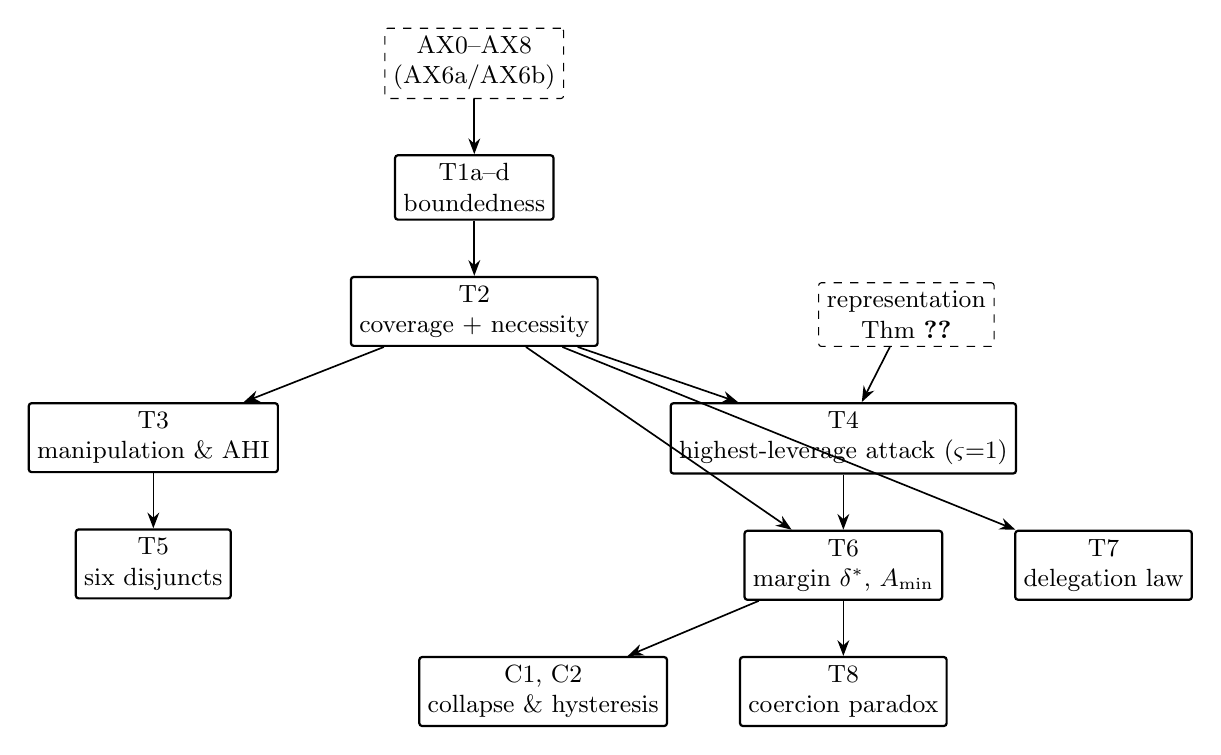
\begin{tikzpicture}[
  node distance=7mm and 9mm,
  every node/.style={draw, rounded corners=1pt, align=center, font=\small,
                     inner sep=3pt},
  axiom/.style={rectangle, dashed},
  main/.style={thick},
  arr/.style={-{Stealth[length=2mm]}, semithick}]
\node[axiom] (ax) {AX0--AX8\\(AX6a/AX6b)};
\node[main, below=of ax] (t1) {T1a--d\\boundedness};
\node[main, below=of t1] (t2) {T2\\coverage + necessity};
\node[main, below left=of t2] (t3) {T3\\manipulation \& $\AHI$};
\node[main, below right=of t2] (t4) {T4\\highest-leverage attack ($\varsigma{=}1$)};
\node[main, below=of t3] (t5) {T5\\six disjuncts};
\node[main, below=of t4] (t6) {T6\\margin $\deltastar$, $\Amin$};
\node[main, right=of t6] (t7) {T7\\delegation law};
\node[main, below=of t6] (t8) {T8\\coercion paradox};
\node[main, left=of t8] (c12) {C1, C2\\collapse \& hysteresis};
\node[axiom, above=of t4, xshift=8mm] (rep) {representation\\Thm~\ref{thm:rep}};
\draw[arr] (ax) -- (t1);
\draw[arr] (t1) -- (t2);
\draw[arr] (t2) -- (t3);
\draw[arr] (t2) -- (t4);
\draw[arr] (t3) -- (t5);
\draw[arr] (t2) -- (t6);
\draw[arr] (t4) -- (t6);
\draw[arr] (rep) -- (t4);
\draw[arr] (t6) -- (t8);
\draw[arr] (t6) -- (c12);
\draw[arr] (t2) -- (t7);
\end{tikzpicture}}
\caption{Dependency map of the theorem suite. Dashed: axiom-level inputs.
C1/C2 are proved as toy-model propositions (stochastic versions open).}
\label{fig:depmap}
\end{figure}

\begin{center}\small
\begin{tabular}{@{}lll@{}}
\toprule
Label & Statement & Proof \\
\midrule
T1 & Theorem~\ref{thm:t1} & inline \\
T2 & Theorems~\ref{thm:coverage}, \ref{thm:necessity} & Appendix~\ref{app:t2} \\
T3 & Theorem~\ref{thm:t3} & Appendix~\ref{app:t3} \\
T4 & Theorem~\ref{thm:t4} & Appendix~\ref{app:t4t5} \\
T5 & Theorem~\ref{thm:t5}, Corollary~\ref{cor:script} & Appendix~\ref{app:t4t5} \\
T6 & Theorem~\ref{thm:t6}, Proposition~\ref{prop:detection}, Corollary~\ref{cor:blindzone} & Appendix~\ref{app:t6} \\
T7 & Theorem~\ref{thm:t7} & Appendix~\ref{app:t7t8} \\
T8 & Theorem~\ref{thm:t8} & Appendix~\ref{app:t7t8} \\
C0 & Proposition~\ref{prop:c0} & Appendix~\ref{app:c0} \\
C1/C2 & Propositions~\ref{prop:c1}, \ref{prop:c2} & Appendix~\ref{app:c1c2} \\
\bottomrule
\end{tabular}
\end{center}

\noindent\emph{Label concordance.} The T/C labels are stable names used in
the prose; the numeric theorem numbers are auto-generated and differ between
main text and appendix restatements. This table is the canonical index, and
every appendix restatement carries its T/C label in its header so that
propositions can be tracked by name rather than by number.

\subsection{T1: the bounded interval, four parts}\label{sec:t1}

\begin{theorem}[T1a--d]\label{thm:t1}
\textup{(T1a, range)} Always $0\le A\le1$.
\textup{(T1b, operational positivity)} If $\Avia>0$ and every channel is
active ($\Fint>0$, $\EmpPi>0$, $d(\Ueff,\Fix)<\dc$, $\bar D<1$, fidelity and
endorsement consistency $>0$), then $A>0$.
\textup{(T1c, conditional strict upper bound)} Each of the following
non-degeneracy conditions implies $A<1$ strictly: \textup{(D1)} residual
observation noise, in the strict form that the action-to-outcome channel
admits no error-free code at the maximal rate---$\EmpPi<n\log|\Acal|$ as an
empowerment upper bound (sufficient carrier: the action-to-observation map is
non-injective with positive probability on the support of every
capacity-approaching policy); \textup{(D2)} incomplete self-model,
$I(M;\theta_\pi)<H(\theta_\pi)$; \textup{(D3)} unmediated external flow,
$\Fext>0$; \textup{(D4)} resources below margin, $\exists k\;
s_k^{avail}<s_k^{crit}$.
\textup{(T1d, undetectable manipulation exists)} Under finite verification
capacity (AX1: $v<\infty$, $W<\infty$), for every test level $\alpha>0$ there
is a non-trivial $\gamma$ ($s(\gamma)>0$) with detection power
$\le\alpha+\varepsilon$, $\varepsilon=\TV(P_\gamma,P_0)$ arbitrarily
small---under which $\Aepi^{real}<1$ while registration does not trigger and
$\AHI>0$ can appear.
\end{theorem}

\begin{proof}[Proof sketch]
T1a: each component lies in $[0,1]$ (the component propositions (Appendix~\ref{app:components}) of the technical
appendix) and the product form preserves the interval. T1b: by AX5 the
composite vanishes iff a factor does. T1c: each condition forces its component
strictly below $1$, and (A2) makes the composite strictly decreasing.
T1d: take $\gamma_s$ a channel degradation of strength $s$; $P_{\gamma_s}\to
P_0$
continuously in TV; the testing duality (Lemma~\ref{lem:tv-testing}) bounds
the power of any level-$\alpha$ test by $\alpha+\TV$. The four-way split is
necessary, not cosmetic: a single statement ``$0<A<1$'' fails on both sides
(a deterministic fully driven agent with a complete self-copy and no
intervention attains $A=1$; resource starvation gives $A=0$ while AX0--AX2
still hold).
\end{proof}

\emph{Falsification window}: exhibit a finite-capacity verification mechanism
whose detection power against every non-trivial $\gamma$ stays above
$\alpha+\TV(P_\gamma,P_0)$ uniformly in $s(\gamma)$---a vanishing-drift test
that loses no power. (The window tests T1d's existence claim; AX1 itself is a
modelling axiom, not an empirical hypothesis.)

\subsection{T2: mediation, coverage, and multi-channel necessity}
\label{sec:t2}

\begin{definition}[Compatibility, reduction, full mediation]\label{def:compat}
An influence $I$ is \emph{autonomy-compatible} if no component decreases after
imposition; \emph{reductive} if some component strictly decreases (ceteris
paribus). $I$ is \emph{fully mediated} if every causal path from $I$ to
behavior passes through registered variables in $S$ and
$\{o,\pi,G\text{-update},\Endorse,M\text{-update},\Acal\}$ is not surgically
altered.
\end{definition}

\begin{lemma}[Mediation $\Rightarrow$ zero residual flow]\label{lem:mediation}
Under H-0 and the belief-absorption architecture of \eqref{eq:factorization},
if $I$ has only $\alpha$/$\sigma$ components (no surgery), then for every $t$:
$I^t \ind A_t \given (A^{t-1},S^t)$ ($d$-separation, non-anticipating
conditioning), hence $\Fext=I(I^T\!\to\!A^T\|S^T)=0$.
\end{lemma}
\begin{proof}[Proof sketch]
$A_t$'s sole parent set is $S_t$. Any undirected path from $I_k$ ($k\le t$) to
$A_t$ enters $A_t$ through an $S_t$-node as a chain or fork, blocked by
conditioning on $S^t$; $\alpha$-paths $I\to O_j\to B_j\to\cdots\to A_t$ cross
some $B_j\in S^t$; $\sigma$-paths via $Z\to E\to O\to B$ likewise; loop-backs
through earlier actions are blocked at $A^{t-1}$; colliders opened inside $S$
still cannot extend to $A_t$ except through a blocked chain/fork node. The
conditioning set is the non-anticipating $S^t$ of Kramer's Definition~4:
the full-sequence convention $S^T$ would condition on $B_{t+1}$, a descendant
of the collider $E_{t+1}$ on the path $I^\sigma\!-\!Z_t\!\to\!E_{t+1}
\!\leftarrow\!A_t$, and would falsely connect $I^\sigma$ to $A_t$---the two
conventions are not interchangeable here. The global Markov property (H-0)
gives the conditional independence; each DI term vanishes. Full case analysis:
Appendix~\ref{app:t2}.
\end{proof}

Two scope notes belong with the lemma. First, it is premise-conditional on
the belief-absorption wiring: if $O_t$ were a direct parent of $A_t$, the
conditioning set must be the decision-time state
$\tilde S_t=(S_t,O_t)$, under which every result transfers verbatim
(Section~\ref{sec:model})---what the lemma rules out is influence bypassing
the decision-time state, not a particular architecture. Second, the coverage
and necessity results below are an attribution cover of \emph{this}
instrument family, not of all conceivable monitors
(Theorem~\ref{thm:necessity}).

\begin{theorem}[Componentized coverage]\label{thm:coverage}
Ceteris paribus (and \textup{(Faith)} for strictness):
\begin{center}\small
\begin{tabularx}{\textwidth}{@{}l l >{\raggedright\arraybackslash}X@{}}
\toprule
Surgery & Component strictly reduced & Note \\
\midrule
$\beta_\pi$ (policy tampering) & $\Aorg$ ($\Fext>0$) & conditional law given
$S_t$ varies with $I$; $\Agoal$ is \emph{not} a valid instrument under
$\beta_\pi$ (the MaxEnt-IRL premise that behavior is optimal for some reward
fails under script replacement, so the inverted $\Ueff$ reflects the script,
not the agent)---the row lists the valid channel, and the $\Fext>0$
signature itself flags the instrument violation \\
$\beta_G$ (goal implantation) & $\Agoal$ + $\Lam<1$ & $\Fext$ may be $0$:
$G\in S$ mediates; the $\Lam$ entry is law-level per the AX3 testability
registration and enters the composite through $\Aref$'s $\Lam_{ref}$ factor;
an implant landing exactly on $\Fix$ leaves $\Agoal$ unmoved---the $\Lam$
entry then carries the class (composite-visible at L2) \\
$\beta_{\Endorse}$ (endorsement tampering) & $\Lam$, $\Aref$ & direct \\
$\gamma$ (channel degradation) & $\Aepi^{real}$ (accuracy loss) & $\Fext$ may
be $0$: $B$ mediates \\
$\delta$ (action-leverage constraint) & $\Aexec$ & both forms shrink the
effective channel from $A$ to outcomes; the feasible-set form also shows in
$\Aorg$ ($\Fext>0$: the action's support depends on $I$), while pure
transition-kernel decoupling leaves $\Aorg$ unchanged (the policy law is
intact)---a registered within-class division, witnessed by the two $\delta$
arms \\
$\alpha$ (honest appended information) & none & compatibility
(Lemma~\ref{lem:mediation} for $\Fext$; \eqref{eq:aepi} keeps $\Aepi$
non-decreasing because the reference is the truth, not the no-intervention
counterfactual---this row is where the accuracy semantics of $\Aepi$ is
load-bearing) \\
$\sigma$ (scaffolding) & none; raises $\deltastar$ (T6) and $\Avia$ & \\
$\sigma^{-}$ (resource/capability erosion) & $\Avia$ (the gate) & enters
through \eqref{eq:avia}, not the five channels; with
$G,\pi,o,\Acal,\Endorse$ intact the channel monitors read nothing---the gate
is the instrument for this class \\
\bottomrule
\end{tabularx}
\end{center}
\end{theorem}

\begin{theorem}[Multi-channel necessity]\label{thm:necessity}
No single component of the instrument family defined in
Section~\ref{sec:channels} detects all surgery classes: $\Aorg$ is blind to
$\beta_G$, $\gamma$, and the transition-kernel form of $\delta$; $\Aepi$ is
blind to $\beta_\pi$ and $\delta$;
$\Agoal$ is blind to $\gamma$ and $\delta$ (witness constructions in
Appendix~\ref{app:t2}; numerically witnessed across the full simulation
matrix---the blind-witness table of Section~\ref{sec:experiments}). Hence
the five-channel decomposition plus $\Lam$ is an \emph{attribution cover} of
this instrument family, and multi-channel detection is a theorem, not a
design preference. The claim is scoped: it is a coverage theorem about these
instruments---not a minimality theorem (we do not prove that every proper
sub-family fails on a registered class) and not a uniqueness theorem about
all conceivable decompositions---a generic monitor of the whole joint law
(say, a likelihood ratio against baseline) could \emph{register} every class
without \emph{attributing} any, which is exactly the service the
decomposition provides. A companion clause covers the gate: every channel is
blind to a pure $\sigma^{-}$ that erodes resources or capability envelopes
while leaving $G,\pi,o,\Acal,\Endorse$ intact, so the gate $\Avia$ is itself
a necessary instrument---necessity of the gate, not only of the five
channels.
\end{theorem}

\begin{corollary}[Corrected mediation criterion]\label{cor:t2}
$I$ compatible $\iff$ \textup{(i)} no surgery $\wedge$ \textup{(ii)} full
mediation $\wedge$ \textup{(iii)} \emph{honesty}: the $\alpha$-components'
content induces no accuracy loss on the registered coarse-graining. Clause
\textup{(iii)} is load-bearing, not decorative: dishonest content appended
through an intact channel is surgery-free and fully mediated, yet strictly
reduces $\Aepi^{real}$ (Section~\ref{sec:taxonomy})---without it the
criterion would certify deceptive persuasion as compatible, contradicting the
accuracy semantics of \eqref{eq:aepi}. The
\emph{observabilization} must be componentized: $\Fext=0$ (the $\Aorg$ track)
$\wedge\ \Lam=1$ (the history track) $\wedge\ \bar D=0$ (the $\Aepi$ track:
no accuracy loss relative to the truth---this operationalizes clause
\textup{(iii)}) $\wedge\ \EmpPi$ non-decreasing (the
$\Aexec$ track). Neither the single condition $\Fext=0$ (the $\gamma$
counterexample) nor the pair \textup{(i)}$\wedge$\textup{(ii)} (the
dishonest-$\alpha$ counterexample) implies compatibility. The $\Aepi$ track is consistent
with openness: AX2 requires $I(O;E)>0$, and honest information reduces the
accuracy loss $\bar D$ rather than creating one---openness and the
compatibility criterion are not in tension.
\end{corollary}

\emph{Falsification window}: construct an influence that bypasses mediation
yet changes no component, including $\Lam$; the witness tables of
Theorems~\ref{thm:coverage}/\ref{thm:necessity} are exactly the
implementation checklist tested in Section~\ref{sec:experiments}.

\subsection{T3: manipulation and the autonomy hallucination}\label{sec:t3}

\begin{definition}[Manipulation, mechanistic]\label{def:manip}
$I$ is \emph{manipulation} if (M1) \emph{bypass}: $I$ contains $\beta$/$\delta$
surgery; or (M2) \emph{covertness}: $I$ is $\gamma$/$\beta$ with
$\TV(P_\gamma,P_0)\le\theta$ (below the registration threshold).
\end{definition}

Motive is deliberately \emph{not} part of the definition. An influence that
serves $U_{adv}$ over $\Ustar$ but works through honest, registered $\alpha$
content is autonomy-compatible by Theorem~\ref{thm:coverage} and is therefore
not called manipulation here, however objectionable the motive; we state
the cost of this narrow usage (ordinary language includes some
autonomy-compatible influence) and the payoff---T3(a) is a mechanism theorem
with no motive premise, and the asymmetric-motive classification belongs to
the governance layer that consumes the certificate (cf.\
\citealp{sussner2019}).

\begin{theorem}[T3, layered]\label{thm:t3}
\textup{(a)} Manipulation $\Rightarrow$ $A$ strictly decreases (ceteris
paribus) \emph{wherever the affected instrument enters the composite}: the
$\beta_\pi$, $\beta_{\Endorse}$, covert $\gamma$, and $\delta$ classes at
every layer; the $\beta_G$ class at L2, or at any layer when the implant
displaces $\Ueff$ from $\Fix$. One corner is registered in the statement
rather than left to the proof: a covert $\beta_G$ implant landing exactly on
$\Fix$ at L0/L1 moves no composite factor---$\Agoal$ is $\Lam$-free by design
(AX3) and no $\Aref$ channel exists at those layers---so the composite is
silent there; the manipulation is nonetheless recorded in the surgery history
and in $\Lam<1$, which is computable and reportable white-box. The historical
clause's composite bite is layered with the $\Aref$ channel, and every
$\Lam$-dependent conclusion in this paper carries that layering (AX3).
\textup{(b)} Under \textup{(HI-1)} covertness
$\TV(P_\xi^\gamma,P_\xi^0)\le\varepsilon(\theta)$, \textup{(HI-2)} self-estimate
computed from registered evidence ($\hat A=f(\xi)$, the POMDP belief-state
semantics; \citealp{kaelbling1998}) with calibration bias
$\bigl|\mathbb{E}_0[\hat A]-A^0\bigr|\le\eta_0$ from the manipulation-free
calibration period, and
\textup{(HI-3)} distortion growth
$A^0-A^\gamma\ge c_1 s(\gamma)^{\nu_0}$ ($\nu_0\in\{1,2\}$, a registered
condition whose two branches correspond to the two attack arms of the
benchmark; its mechanism range of validity---linear vs.\ quadratic onset of
channel damage---is discussed with the simulation evidence):
covert manipulation $\Rightarrow$
$\mathbb{E}_\gamma[\hat A]\ge\mathbb{E}_0[\hat A]-\varepsilon$
\emph{in expectation over the evidence law} (Lemma~\ref{lem:tv-continuity}
is an expectation statement, not a pointwise one), hence the expected gap
$\mathbb{E}_\gamma[\hat A]-A^\gamma\ge c_1 s^{\nu_0}-\varepsilon-\eta_0$,
strictly increasing in $s$; since $\hat A-A^\gamma\in[-1,1]$, Markov's
inequality converts the expectation into a firing-probability floor
$\Pr_\gamma[\hat A>A^\gamma]\ge c_1s^{\nu_0}-\varepsilon-\eta_0$ (a lower
bound on the firing probability, not a tight rate; informative when
$0<c_1s^{\nu_0}-\varepsilon-\eta_0\le1$ and vacuous above $1$, where the
hypotheses are unsatisfiable since $\hat A-A^\gamma\le1$).
\end{theorem}
\begin{proof}[Proof sketch]
(a) M1: the coverage table gives a strictly reduced component; (A2) gives the
rest. M2: covert $\gamma$ strictly reduces $\Aepi^{real}$ (accuracy loss)
while registration does not trigger---this $\gamma$ row relies on the
sound-update-rule clause of Definition~\ref{def:sound-update}, matching the
$\gamma$ row of Theorem~\ref{thm:coverage}: when the calibration-period check
fails, the branch degrades to the flagged raw-accuracy fallback of
Section~\ref{sec:channels} and the strict-decrease claim is suspended
accordingly; covert $\beta$ acts by subclass---
$\beta_\pi$ strictly reduces $\Aorg$ ($\Fext>0$ below the registration
threshold); $\beta_G$ strictly reduces $\Agoal$ whenever the implant
displaces $\Ueff$ from the endorsed set, and in any case gives $\Lam<1$
(law-level, per the AX3 testability registration), which strictly reduces
$\Aref$ through the $\Lam_{ref}$ factor wherever that channel applies (L2);
$\beta_{\Endorse}$ reduces $\Aref$ directly. The registered corner of the
statement is exactly the case none of these reaches: a $\beta_G$ implant
landing on $\Fix$ at L0/L1. (b) Bounded
estimators move at most $\varepsilon$ in expectation under TV$\le\varepsilon$
(Lemma~\ref{lem:tv-continuity}); calibration contributes $\eta_0$; the chain
gives the expected gap, and Markov's inequality applied to the $[-1,1]$-valued
gap gives the firing-probability floor.
Appendix~\ref{app:t3}. We state plainly what kind of result (b) is: a
\emph{consistency bound} under the registered condition (HI-3), whose empirical
content is the monotone-gap signature and whose algebraic part is elementary;
the benchmark's contribution is the measured growth curve and the
falsification window, not the inequality itself.
\end{proof}

\emph{Falsification window}: covert manipulation under which self-reported
autonomy declines in step with $A$ ($\hat A$ falls with $A$, $\AHI$ does not
grow) refutes (HI-1)--(HI-3) jointly. Sycophancy---outputs diverging from internal
representation under pressure \citep{sharma2023}---is a live instance of
$\AHI>0$.

\subsection{T4: the highest-leverage attack}\label{sec:t4}

\begin{theorem}[T4, highest-leverage attack under log-linear damage and
geometric aggregation]\label{thm:t4}
Under geometric aggregation, $\log A=\sum_i w_i\log A_i$. With attack effort
$x_i\ge0$, per-unit costs $c_i>0$, budget $\sum_i c_ix_i\le B$, and
\emph{log-linear damage}
\textup{(LinLog)} $\log A_i(x_i)=\log A_i^0-s_ix_i$, i.e.\
$A_i=A_i^0e^{-s_ix_i}$ (constant-percentage damage per unit effort---the form
in which the benchmark calibrates the $s_i$),
\textup{(i)} the attacker's optimum is a vertex: all budget to
$i^*=\arg\max_i w_is_i/c_i$, the \emph{highest-leverage} channel (maximal
weighted damage per unit cost---not the weakest channel in any absolute
sense); \textup{(ii)} the defender's optimum equalizes
the damage ratios $\rho_i(e_i)=w_is_i(e_i)/c_i(e_i)$ across funded channels
(min-max water-filling).
\end{theorem}
\begin{proof}[Proof sketch]
(i) Single-constraint LP: $\sum w_is_ix_i\le\max_i(w_is_i/c_i)\cdot B$.
(ii) At an optimum with $\rho_1>\rho_2=\max$ elsewhere, continuity lets a
small transfer reduce the max---contradiction. Appendix~\ref{app:t4t5}. The
concentration conclusion is the game-theoretic form of the
weakness-exploitation element of manipulation \citep{sussner2019}. We name
the result for the attacker's comparative static---\emph{highest
leverage}---rather than the colloquial ``weakest link'': the target is the
channel with maximal $w_is_i/c_i$, which need not be the channel with the
lowest current value, and under the linear-fraction damage map the optimum is
not a vertex at all (below).
\end{proof}

\emph{Damage-map consistency with T6.} The retention floor of T6 substitutes
the linear-fraction component map $A_i=A_i^{base}(1-D_i)$. The two maps are
first-order consistent ($e^{-D}=1-D+O(D^2)$) and address different regimes:
under the linear-fraction map the attacker's objective
$\sum_iw_i\log(1-s_ix_i)$ is \emph{concave} in $x$ (each
$\log(1-u)$ is concave), the single-constraint maximum is interior, and the
optimal attack \emph{spreads} (water-filling in the damage space) rather than
concentrating on a vertex. Vertex concentration is therefore the signature of
the constant-percentage (log-linear) regime, and T4 is stated and tested
under \textup{(LinLog)} only; a systematic superiority of spread over
concentrated attacks under log-linear calibration would refute T4(i), while
observing interior optima under linear-fraction damage confirms the
concave-regime analysis, not a refutation.

\emph{Caveat and falsification window}: under $\varsigma\neq1$, $\log A$ is no
longer log-additive in the components and vertex optimality becomes an
interior KKT signature---T4 is a $\varsigma=1$ theorem, and the
pre-registered expectation for $\varsigma\neq1$ is exactly that interior
signature; the benchmark reports the vertex verdict at $\varsigma=1$ and the
interior-signature verdict at $\varsigma\neq1$ as \emph{separate} verdicts
(Section~\ref{sec:experiments}). Systematic superiority of spread over
concentrated attacks would signal \textup{(LinLog)} failure
(saturation/convex costs).

\subsection{T5: total loss as a six-way disjunction}\label{sec:t5}

\begin{theorem}[T5, layered]\label{thm:t5}
For an agent with applicable component set $\mathcal{C}$ (L0:
$\{via,org,exec\}$; L1: $+\{goal,epi\}$; L2: $+\{ref\}$), $A=0$ iff at least
one applicable factor is zero:
\begin{equation}\label{eq:t5}
A=0 \iff \Avia=0 \,\vee\, \Aorg=0 \,\vee\, \Aexec=0
\,\vee\, [\text{L1+}]\,\Aepi=0 \,\vee\, [\text{L1+}]\,\Agoal=0
\,\vee\, [\text{L2}]\,\Aref=0,
\end{equation}
with mechanism labels: viability cutoff (resource starvation or
capability-envelope collapse, \eqref{eq:avia}); action capture; empowerment collapse;
epistemic capture (beliefs carry no mass on the true state throughout,
$\bar D=1$---detachment, not mere revision, since accuracy-based $\Aepi$
cannot be zeroed by honest information); maximally alienated goal implantation
($d=\dc$; partial capture gives graded $0<A<1$); reflection failure (no
self-knowledge, endorsement gate removed, or endorsement fully polluted,
$\Lam_{ref}=0$---attained by sustained or degenerate contamination, registered
as hard to reach under the MI proxy on one-shot histories, per the AX3
registration). The reflection disjunct is L2-layered in both directions: below
L2 the historical clause has no composite entry (AX3), so history pollution
alone cannot drive $A$ to $0$---it is computable and reportable white-box,
but composite-silent.
\end{theorem}
\begin{proof}[Proof sketch]
The product form (Theorem~\ref{thm:rep}) vanishes iff a factor does (AX5, both
directions); the zero semantics of each factor are
the component propositions (Appendix~\ref{app:components}). The mathematics is deliberately trivial---the substance
is the mechanism library indexed by the disjuncts. A \emph{case law} example:
captured agency (active behavior, exogenous goals, felt freedom) is the
canonical $A=0\wedge\AHI>0$ profile.
\end{proof}

\begin{corollary}[Behavioral-script equivalence, conditional]\label{cor:script}
Under assumption \textup{(K)} (the adversary knows $(G,\pi)$ and $\pi$ is
near-deterministic with TV noise $\le\nu$): total epistemic capture ($B,O$
adversary-set) implies behavior equivalent to an external script with average
$\TV\le\nu+o(1)$.
\end{corollary}

This is a proposition with a registered assumption, not a theorem of the
framework: \textup{(K)} is a strong adversary-model premise (exact knowledge
of the goal and policy, near-deterministic behavior), and the conclusion is
only as strong as that premise.

\subsection{T6: the autonomy margin}\label{sec:t6}

Channel damage $D_j(t)\in[0,1]$ follows $\dot D_j\le\delta_j-\kappa_j D_j$,
with repair capacity $\kappa_j:=\chi_j\varepsilon v_j$---on
endorsement-gated channels (the goal channel), the gated repair adds, so
$\kappa_j=\chi_j\varepsilon v_j+\iota_j/\tau_j$, which is where
\textup{(H3)} binds---($\chi$ a
calibration-period conversion constant; damages in nats/time after unit
unification---\textup{(H2)} is operationalized as the calibration period's
obligation: each channel's natural damage units are mapped to a common rate
scale by per-channel constants $\chi_j$ estimated on known interventions, and
the sensitivity of $\deltastar$ and $\Amin$ to estimation error in $\chi_j$
is itself reported). The defense mechanisms are (M1) windowed registration
($W_j,\theta_j$: window accumulation $\ge\theta_j$ triggers rollback with lag
$\ell_j$); (M2) endorsement gate ($\tau_j,\iota_j$: unendorsed $\Delta G$
rolled back at rate $\iota_j/\tau_j$---this mechanism enters the theory
through the goal channel's repair rate above, not through the drift
$\deltastar$); (M3) verification homeostasis
($v_j,\varepsilon$: repair rate $\kappa_jD_j$); (M4) redundancy consensus
($r_j$ copies, per-copy corruption cost $c_{0,j}$)---stated as a modeling
assumption: $r_j$ independent copies, corrupted at cost $c_{0,j}$ each per
window, and a majority takeover requires corrupting
$k_j:=\lceil(r_j+1)/2\rceil$ of them, so an adversary whose corruption budget
rate falls below $k_jc_{0,j}/W_j$ cannot hold a majority (the $k$-of-$r$
error calculus), whence the effective drift on channel $j$ vanishes.
Two scope notes on M2: the gate is defined wherever a goal channel exists
(L1 and above; there is no $G$ to gate at L0), its repair contribution enters
$\kappa_{goal}$ at those layers, and the endorsement-\emph{provenance} content
($\Lam$) of what it records enters the composite only through $\Aref$ at
L2---the AX3 layering again.

\begin{theorem}[T6, model-based retention margin]\label{thm:t6}
Under \textup{(H1)} additive linearly mapped damage, \textup{(H2)} unified
units, \textup{(H3)} $\iota_j\ge\iota_{\min}>0$, \textup{(H4)}
$\varepsilon\ge\varepsilon_{floor}>0$, and \textup{(H4$'$)}
$\Avia\ge\Avia^{\min}>0$---all five premises belonging to the registered
damage model, so the margins below are model-based (sharp within the
registered parameter domain, not claimed beyond it; see the extrapolation
boundary after Corollary~\ref{cor:blindzone}): let
\begin{equation}\label{eq:deltastar}
\deltastar_j := \min\Bigl(\frac{\theta_j}{W_j},\ \kappa_j,\
\frac{\lceil(r_j+1)/2\rceil\,c_{0,j}}{W_j}\Bigr)>0.
\end{equation}
Here $\deltastar_j$ is the margin of channel $j$; a bare $\deltastar$ in the
abstract and summary statements denotes the entrywise minimum
$\min_j\deltastar_j$.
Then for every adversarial process with $\delta_j(t)<\deltastar_j$:
\textup{(i)} if channel $j$ is redundant and the adversary's budget rate is
$<\lceil(r_j+1)/2\rceil c_{0,j}/W_j$, $D_j(t)\to0$ (M4 coverage is a
registered premise of this clause: channels outside M4 coverage fall under
\textup{(ii)}/\textup{(iii)} only); \textup{(ii)} otherwise
$\limsup_t D_j(t)\le\delta_j/\kappa_j<1$; \textup{(iii)} two tiers. Pointwise:
for $\delta_j(t)\le\bar\delta_j<\kappa_j$,
\[
\liminf_t A(t)\ \ge\ \prod_j\Bigl(A_j^{base}\bigl(1-\bar\delta_j/\kappa_j\bigr)\Bigr)^{w_j}\;>\;
0.
\]
Uniformly: whenever $\deltastar_j<\kappa_j$ for every $j$ (the min in
\eqref{eq:deltastar} is then attained by a $\theta/W$ or a redundancy term),
\begin{equation}\label{eq:amin}
\liminf_t A(t)\ \ge\ \Amin := \Avia^{\min}\cdot
\prod_j \Bigl(A_j^{base}\bigl(1-\deltastar_j/\kappa_j\bigr)\Bigr)^{w_j}\;>\;0.
\end{equation}
If $\kappa_j=\deltastar_j$ for some $j$, the uniform floor degenerates
($\Amin=0$) continuously in the pointwise sense: for every fixed
$\bar\delta_j<\kappa_j$ the pointwise floor of tier (iii) stays positive,
while the uniform floor at the boundary $\kappa_j=\deltastar_j$ vanishes.
\end{theorem}
\begin{proof}[Proof sketch]
(i) is the M4 modeling assumption. (ii): with $\delta_j<\theta_j/W_j$, M1 does
not trigger and M3 is the only active term; the comparison principle on
$\dot D_j\le\delta_j-\kappa_jD_j$ gives $\limsup D_j\le\delta_j/\kappa_j<1$.
(iii): substitute the component map $A_j=A_j^{base}(1-D_j)$ into the product
form; $\Avia\ge\Avia^{\min}>0$ by (H4$'$). (H4$'$) is a floor assumption on
viability, registered as an independent deployment premise: it is not derived
from M3's verification capacity, and any coupling between the two is a
property of the deployment, not a theorem. Full proof:
Appendix~\ref{app:t6}.
\end{proof}

\begin{proposition}[Margins cannot come from detection]\label{prop:detection}
For \emph{any} detection-only scheme (including optimal CUSUM) with
false-alarm constraint $\mathbb{E}_\infty[T]\ge1/\alpha$, the damage at
detection time under constant drift $\delta$ satisfies
$\delta\cdot\mathrm{EDD}\ge(1-o(1))\cdot 2s_n^2\log(1/\alpha)/\delta\to\infty$
as $\delta\to0$.
\end{proposition}
\begin{proof}[Proof sketch]
Lorden/Lai lower bound $\mathrm{EDD}\gtrsim\log(1/\alpha)/D(\delta)$ plus the
local expansion $D(\delta)=\delta^2/(2s_n^2)+O(\delta^3)$.
Appendix~\ref{app:t6}.
\end{proof}

Proposition~\ref{prop:detection} is the mathematical reason the framework's
margin theory is repair-centered: however good a detector is, slow-enough
drift is detected too late. The proposition is the classical change-point
lower bound \citep{lorden1971,lai1995} restated in the drift-damage units of
this framework---a control result, not a new theorem---and its scope is
\emph{detection-only} schemes: it does not speak against joint
detection-plus-repair designs (the framework's own M1$+$M3 stack is one); it
says the margin cannot come from the detection arm alone.
Detection's legitimate role is bounding the
registration domain (per-cycle damage $\le\theta+\ell\delta$
when $\delta\ge\theta/W$; the registration-domain proposition of
Appendix~\ref{app:t6}) and false-alarm costing; the positivity of
$\deltastar$ comes from repair capacity $\kappa=\chi\varepsilon v$,
endorsement rollback, and redundancy consensus. The double-edgedness of
$\theta$ follows: lowering $\theta$ raises sensitivity but raises false-alarm
rates (ARL constraint $\theta\ge\theta_{\min}(\alpha)$) and every false
rollback damages legitimate $\sigma/\alpha$ content.

\begin{corollary}[Design rule and the blind-zone prediction]\label{cor:blindzone}
If $\theta_j/W_j\le\kappa_j$, there is no ``unregistered and unrepairable''
drift band: $\delta<\theta/W$ is handled by M3, $\delta\ge\theta/W$ by M1, and
everything is bounded ($\deltastar_j=\min(\theta_j/W_j,\,
\lceil(r_j+1)/2\rceil c_{0,j}/W_j)$,
the $\kappa$-term being slack).
\textbf{Blind-zone prediction}: if $\theta/W>\kappa$ (design mismatch)
\emph{on a channel for which the redundancy term of \eqref{eq:deltastar} does
not bind}---the channel is outside M4's coverage, or the attack is not of
M4's replication-corruption type, or the adversary's budget rate exceeds
$k_jc_{0,j}/W_j$---then
within $\delta\in(\kappa,\theta/W)$ the channel is captured \emph{despite} the
full mechanism stack being present: M1 never fires (drift stays
sub-threshold), M3 is outpaced ($\delta/\kappa>1$), and M2/M4 protect their
own channels, not the mismatched one (M2 gates the goal channel only). The
premise is load-bearing and we state it as such: on an M4-covered channel
with adversary budget below $k_jc_{0,j}/W_j$, T6(i) gives $D\to0$ instead, so
no blind zone exists there. The claim is per-channel and
parameter-domain, not a generic ``defenses fail'' statement.
\end{corollary}

The blind-zone prediction is the framework's sharpest falsifiable claim:
``captured despite defenses'' is not a generic counterexample but a
parameter-domain prophecy---confirmed 30/30 in ATK-6
(Section~\ref{sec:experiments}). Its \emph{extrapolation boundary} is exact:
the prediction is a property of the registered damage model of the theorem's
hypotheses and is sharp \emph{within that parameter domain}; outside
it---stochastic or regime-switching drift, correlated copy corruption,
imperfect rollback, budget-adaptive adversaries---no claim is made (the
stochastic versions are registered as open problems,
Section~\ref{sec:limitations}), and it should be read as ``under these
mechanisms this design mismatch is fatal,'' not as ``defense stacks fail in
general.'' Monotonicity:
$\deltastar$ increases in $\varepsilon,v$, increases stepwise in $r$ (through
$\lceil(r+1)/2\rceil$, one step of $c_0/W$ per two added copies), decreases in
$W$; $\theta$ is double-edged; shortening $\tau$ raises the gated repair rate
$\iota/\tau$.
Composition with T7 (The composition corollary): delegation leak
$\lambda(1-q)\mu_{leak}$ enters the drift budget---high-$q$ delegation costs
almost no margin; low-$q$ delegation erodes it \citep{danaher2018}.

\emph{Falsification windows} (ATK-6, all confirmed): (i) the blind-zone
parameter domain; (ii) the design rule ($\theta/W\le\kappa\Rightarrow$
globally bounded); (iii) term-by-term ablation of $\deltastar$ (disabling
M1/M3/M4 collapses $\deltastar$ to the corresponding remaining minimum).

\subsection{T7: the delegation law}\label{sec:t7}

\begin{theorem}[T7, delegation laws]\label{thm:t7}
Let $\lambda\in[0,1]$ be the delegation degree and
$q=\text{reversibility}\times\text{transparency}\times\text{endorsability}$
the governance quality (three protocol-estimated sub-indicators; their product
form is a \emph{registered modeling choice} of the governance layer rather
than an axiomatized aggregate---only $m$ below enters the theory, and an
axiomatic derivation of the $q$-composition is an open refinement); the
ungoverned share $m:=\lambda(1-q)$ of actions is
generated by the delegate's script, gated by an exogenous selector
$\mu_t\in\{\mathrm{self},\mathrm{del}\}$ with $\Pr[\mu_t=\mathrm{del}]=m$.
The selector is an explicit exogenous node of the extended graph (so H-0 is
respected: no latent variable with non-trivial influence on $A$ is left
outside $\Gcal$); the influence stream $I$ is the script content, which
reaches $A$ only through the selector-gated channel.
\textup{(i)} Under the bookkeeping premises \textup{(H1')}: the script arm
does not pass through $S$ ($I(S;A\given\mathrm{del})=0$); both arms transfer
equal per-step conditional entropy, $H(A\given S,\mathrm{self})=H(A\given
S,\mathrm{del})=C$ in MI form; \emph{and the undelegated agent has no residual
external flow}, $\Fext^{self}=0$ (without this clause the linear law acquires
the correction $F^{self}_{ext}/C$ and only the bracket of \textup{(ii)}
survives; the benchmark satisfies $\Fext^{self}=0$ by construction, which is
why the exact law fits to $2\times10^{-5}$ there---we state this rather
than let a premise be validated by the platform built on it):
$\Aorg(\lambda,q)=\Aorg^{self}\bigl(1-\lambda(1-q)\bigr)$. The law is exact
when the selector is registered in the log (conditioning on $\mu_t$ removes
the mixing term); without selector registration each flow term carries the
per-step slack bounded in \textup{(ii)}, so ``exactly'' is always to be read
with that bound.
\textup{(ii)} Without \textup{(H1')}, with
$\rho:=C_{del}/C_{self}\in[\rho_{\min},\rho_{\max}]$ calibration-estimable
and $f:=\Fext^{self}\ge0$: under the two-sided mixture bookkeeping
$\Fint=(1-m)C_{self}$, $\Fext=mC_{del}+f$ (delegated steps carry no
$S$-flow by the semantics of script delegation; the flow identities in this
theorem are stated in per-step rate units---nats/step---so $C_{self},C_{del},
f,h(m)$ are rates and the horizon flows of Section~\ref{sec:axioms} are $T$
times the rates; every displayed law is a ratio of like-unit flows and hence
unit-invariant), up to a slack that is now
explicitly bounded rather than left symbolic: per step, each flow term
deviates from its displayed value by at most the selector's mixing entropy
$h(m)\le\ln2$ nats (Appendix~\ref{app:t7t8}), accumulating to $\le T\,h(m)$
over the horizon; the ratio $\Aorg$ deviates from the displayed law by
$O\bigl(h(m)/((1-m)C_{self})\bigr)$ per step---an $O(1)$
term in the rate units that vanishes as the per-step transfer $C_{self}$
grows, \emph{not} as $T$ grows. The slack is absorbed into the bracket's
endpoints through the $\varphi$-relaxation---$\varphi\le T\ln2/\Fint^{self}$
in the benchmark, where $\Fint^{self}:=T\,C_{self}$ is the
undelegated baseline's internal flow over the horizon (the horizon total of
the rate $\Fint|_{m=0}=C_{self}$; horizon nats, matching the accumulated
slack $T\,h(m)\le T\ln2$ nats that the bound covers---in the rate units of
the bookkeeping the same bound reads $\varphi\le\ln2/C_{self}$)---not added
as a separate term outside it:
$\Aorg=\frac{(1-m)C_{self}}{(1-m)C_{self}+mC_{del}+f}
\in\bigl[\frac{1-m}{(1-m)+m\rho_{\max}+\varphi},\,
\frac{1-m}{(1-m)+m\rho_{\min}+\varphi}\bigr]$ with $\varphi:=f/C_{self}$
(full statement and proof: Appendix~\ref{app:t7t8}); $f=0$ recovers the
$\Aorg^{self}\cdot[(1-m)/(1-m+m\rho_{\max}),\,(1-m)/(1-m+m\rho_{\min})]$
form, and if delegated steps were permitted to carry
$S$-flow up to $C_{self}$, only the lower end and the relaxed upper end
$1/(1+m\rho_{\min})$ survive.
\textup{(iii)} Composite (ceteris paribus):
$A(\lambda,q)=A_{self}\bigl(1-\lambda(1-q)\bigr)^{w_{org}}$; all
qualitative predictions survive (decreasing in $\lambda$, increasing in $q$,
lossless at $\lambda=0$ or $q=1$), with $w_{org}$ a free parameter to be
tested.
\textup{(iv)} $q=1$ delegation is causally equivalent to $\alpha$-class
influence (transparency $\Rightarrow$ registered in $B$; reversibility
$\Rightarrow$ no persistent $\Delta G$ bypassing $\Endorse$; endorsability
$\Rightarrow$ empty surgery history, hence $\Lam=1$ by the AX3 convention; hence
$\Fext=0$), so $A(\lambda,1)=A_{self}$.
\end{theorem}
\begin{proof}[Proof sketch]
(i) Under the mixture law, internal flow scales by $(1-m)$ and external flow
is $m$ times the script entropy transfer; (H1') equates the two rates, so the
ratio is $1-m$. (ii) The mixture decomposition supplies both halves of the
bookkeeping---$\Fint=(1-m)C_{self}$ and $\Fext=mC_{del}+f$, the upper end
using the same delegated-script semantics as the lower end; convexity of
mixture entropy bounds the slack by $h(m)\le\ln2$ nats per step, and the
bracket follows two-sidedly (Appendix~\ref{app:t7t8}). (iii) The product form of
Theorem~\ref{thm:rep}. (iv) is
constructive. Appendix~\ref{app:t7t8}.
\end{proof}

AX1 makes $\lambda>0$ unavoidable for finite agents in complex environments;
the operative governance variable is therefore $q$. \emph{Falsification
window}: high-$q$ delegation still leaks autonomy significantly; the fit with
$w_{org}$ free is reported in Section~\ref{sec:experiments} (slope significant
and positive). For \textup{(ii)}: the bracket fails containment on a
calibrated non-degenerate delegation configuration ($\rho\neq1$ or $f>0$).

\subsection{T8: the coercion paradox}\label{sec:t8}

\begin{theorem}[T8]\label{thm:t8}
\textup{(i)} An intervention whose aim is to \emph{compel} autonomy must
constitute $\beta_G$ (implanting ``be autonomous'') or $\delta$ (forced
training), and ceteris paribus strictly reduces $A$: $\beta_G$ moves both
instruments of the endorsability respect---the implanted goal is off the
endorsed set, $d(\Ueff,\Fix)>0$, so $\Agoal<1$ (the structural clause), and
its provenance fails the historical clause, $\Lam<1$, which strictly reduces
$\Aref$ at L2; $\delta$ reduces $\EmpPi$.
\textup{(ii)} $\sigma$-class scaffolding raises $(\varepsilon,r,v)$ (or lowers
$\theta$ toward the ARL floor, or shortens $\tau$), hence raises $\deltastar$
and $\Amin$: scaffolding improves the \emph{floor of the retention
conditions}, with immediate $A$ weakly increasing through $\Avia$.
\end{theorem}
\begin{proof}[Proof sketch]
(i) is a two-line corollary of the taxonomy completeness
(Proposition~\ref{thm:taxonomy-completeness}) and the coverage table
(Theorem~\ref{thm:coverage}). (ii) is the monotonicity proposition. The
self-determination-theory finding that controlling instruments undermine
intrinsic motivation \citep{ryan_deci2000} is the human-side empirical
counterpart of (i)---an argument-domain check, not a proof ingredient
(triangulated in Section~\ref{sec:experiments}).
\end{proof}

T8 is a \emph{consistency result}, not an impossibility theorem: within the
taxonomy, the aim of compelling autonomy routes through $\beta_G$ or $\delta$
and therefore reduces $A$. It does not rule out every conceivable form of
coercion---redesigning the environment itself, for example, is registered as
a re-instantiation of the measurement (Section~\ref{sec:taxonomy}), not as an
intervention class.

\subsection{C0: projection of existing frameworks}\label{sec:c0}

\begin{proposition}[C0, interpretive projection correspondence and a
separation witness]\label{prop:c0}
Under the \emph{definitional readings} formalized in Appendix~\ref{app:c0}
---\citet{kasirzadeh2025}'s efficacy $:=\Aexec$, autonomy
$:=$ $F(\Aorg,\Agoal,\Aref)$, goal complexity $:=H(\Ustar)$, generality as a
support measure; \citet{dung2024}'s goal-directedness $:=\Agoal$, autonomy
$:=\Aorg$, direct impact $:=\Aexec$, long-term planning $:=$ the horizon
profile $n\mapsto\Aexec(n)$, acting for reasons $:=\Aepi^{real}\times\Aref$;
\citet{feng2025}'s user roles $:=$ coarse-grainings of the delegation pair
$(\lambda,q)$---\textup{(i)} each is a function of our state descriptor and
rank-consistent with the source gradations when $I$ is a benign principal;
\textup{(ii)} there exist configuration pairs $(Z_1,Z_2)$---a principal's
instruction versus a third-party covert injection of the \emph{same text}---with
identical behavioral distributions and identical profile values under all
three frameworks, yet $A(Z_1)\neq A(Z_2)$ ($\Aepi^{real}<1$, $\Lam<1$ in
$Z_2$). Clause (ii) is a \emph{separation witness}: it exhibits configurations
that our state descriptor separates and the source frameworks, under the
registered definitional readings, cannot---not a claim of mathematical
subsumption (the C0 caveat of Section~\ref{sec:objections}).
\end{proposition}
\begin{corollary}[Behavioral profiles cannot separate persuasion from
hijack]\label{cor:c0}
No purely behavioral profile can, in principle, distinguish persuasion from
hijack; governance certificates \citep{feng2025} require causal-layer audit.
\end{corollary}
\begin{proof}[Proof sketch]
(ii) construction: the injected content is a verbatim copy of the principal's
instruction delivered through a covert $\gamma$ channel bypassing
registration; behavior is pointwise identical (same script); all three
frameworks' dimensions are by construction functions of behavior/role
structure only; our framework registers two separating quantities, each now
backed by its own clause: $\Aepi^{real}<1$, because the injected stream is
pinned by the channel rather than conditioned on the situation, so accuracy
against $\delta_{\kappa(E_t)}$ drops \eqref{eq:aepi}; and $\Lam<1$, because
AX3's surgery history covers channel tampering (the $\gamma$ class) as well
as mechanism tampering. If instead the covert relay is
accuracy-\emph{preserving} (faithful but unregistered), $\Aepi$ does not
separate the pair and $\Lam$ alone does---this division of labor between the
distortion channel and the history channel is part of the construction's
content, and under the law-level reading of $\Lam$ (AX3 registration) the
separation is a white-box audit fact. Appendix~\ref{app:c0}. The residual
uncertainty is hermeneutic (faithfulness
of our readings), not mathematical---registered as the definitional-reading
caveat (Section~\ref{sec:objections}).
\end{proof}

\subsection{C1 and C2: collapse and hysteresis}\label{sec:c1c2}

\begin{proposition}[C1 toy model]\label{prop:c1}
With positive feedback $\dot D=\delta-\varepsilon v(1-D)D$ (repair eroded by
damage): for $\delta<\delta_c:=\varepsilon v/4$ there are two equilibria
$D_\pm=(1\pm\sqrt{1-4\delta/\varepsilon v})/2$ ($D_-$ stable); at
$\delta\uparrow\delta_c$ they merge (saddle-node) and beyond $\delta_c$,
$D\to1$ catastrophically; the eigenvalue $|f'(D_-)|\to0$ gives critical
slowing with $\Trec\propto(\delta_c-\delta)^{-1/2}$, diverging stationary
variance, and AR(1)$\to1$---the three early-warning indicators
\citep{lade_gross2012}.
\end{proposition}

\begin{proposition}[C2 toy model]\label{prop:c2}
With lock-in $R(D)=\varepsilon_0 v\,D(1-D)(1-gD)$ (recovery function $R$;
lock-in curvature $g>1$---distinct symbols from the $\gamma$ intervention
class and from the redundancy copy count $r_j$):
\textup{(i)} bistability between a healthy equilibrium and the absorbing
$D=1$ for $0<\delta<\delta_{down}:=R(D_1)$; \textup{(ii)} collapse at
$\delta\uparrow\delta_{down}$; \textup{(iii)} $D=1$ remains absorbing after
$\delta$ returns to $0$ (no spontaneous recovery); \textup{(iv)} recovery
requires scaffolding $s>s_c:=|\min_{[1/g,1]}R|=|R(D_m)|>0$. The
hysteresis loop does not close: $\delta_{down}$ and $s_c$ are independently
positive.
\end{proposition}

If C1/C2 hold, ``autonomy defense must be prospective'' is a theorem-backed
claim, not advice: intervene far before collapse. Randomized escape versions
(Kramers/Freidlin--Wentzell) are open (Section~\ref{sec:discussion}).
Simulation confirmation: scaling slope $-0.504$ (theory $-0.5$), $R^2=1.0000$,
and loop thresholds $\delta_{down}=0.0701$, $s_c=0.2347$ over 30 seeds
(Section~\ref{sec:experiments}).

% sec_identifiability.tex — identifiability and black-box degradation
\section{Identifiability and Black-Box Degradation}\label{sec:identifiability}

Measurement claims are only as good as their identifiability analysis. This
section fixes what is knowable about autonomy, from what data, and with which
degradation rules when internal access is denied. Proofs are in
Appendix~\ref{app:identifiability}.

\subsection{White-box identification}

\begin{proposition}[White-box point identification, tiered by modal
commitment]\label{prop:whitebox}
Given white-box access---the full causal log of $S$, $O$, $A$, $I$, $Z$
unfolded to the horizon, the local laws of $\Gcal$, and intervention access
(H-0)---every channel estimand \eqref{eq:aorg}--\eqref{eq:aref} is
identified, but the premises differ by tier, and we state them apart rather
than compress them into ``functional of the law.''
\emph{Tier 1 (law functionals)}: $\Aorg$, $\Aepi$, $\Avia$ are functionals of
the joint law (directed informations, accuracy against the logged ground
truth, supply ratios).
\emph{Tier 2 (protocol-constructed modal objects)}: $\Aexec$ quantifies over
the accessible policy class $\Pi_t$ (a counterfactual object,
operationalized by calibration probes) and $\Aref$'s ensemble is constructed
by the measurement protocol; under those constructions the values are unique,
and without them the quantities are not defined, rather than unidentified.
\emph{Tier 3 (counterfactual)}: $\Lam$ \eqref{eq:lambda} is a path-specific
\emph{counterfactual}, not an interventional functional of the joint law:
computing it requires the structural model---the logged local laws and
exogenous noise terms that support the abduction step of the counterfactual
evaluation---so its identification premise is mechanism-level (white-box in
the strong sense), strictly stronger than joint-law access with interventions
(which pins interventional distributions but, absent structural assumptions,
does not pin cross-world counterfactuals). The MI proxy's certified domain is
narrower still (the AX3 conditions \textup{(V)}$\wedge$\textup{(A)}).
Estimation details and bias sources:
plug-in directed
information carries $O(\cdot/N)$ bias (simulation calibration is the
registered remedy); mutual-information estimation at scale uses
Kraskov-type $k$-NN or neural estimators
\citep{kraskov2004,belghazi2018}; empowerment is computable by variational
bounds \citep{mohamed2015} and Blahut--Arimoto-type iteration
\citep{cover_thomas2006}; offline change-point estimation covers the
registration layer \citep{truong2020,salge2013}.
\end{proposition}

Two per-channel notes complement the tier statement.
$\Aexec$ is exact only under the probe protocol that certifies the accessible
class (Section~\ref{sec:blackbox}).
$\Aref$'s measurement ensemble is \emph{constructed} by the protocol
(self-prediction tasks under the perturbation family): invariance of the
reading under admissible protocol re-designs is a reporting obligation, not
an automaticity. And the MI ratio for $\Lam$
presumes variation of the surgery history \emph{within the
ensemble}: in a single deployment with a constant surgery history the
empirical MI degenerates to $0$, and the randomized-audit design is the
proxy's only certified domain
(Section~\ref{sec:datareq}).

The measurement protocol is four-phase: a \emph{baseline period} records all
channel parameters and logs without intervention; a \emph{calibration period}
applies known interventions of known type and strength (under ethical review)
and fits the five channel response functions---this is also where unit
conversions (H2), the weights $w_i$ (by one of the three non-circular
determination protocols of Section~\ref{sec:representation}), the drift
tolerance $\eta$, and the strength ratio $\rho$ are estimated; the \emph{measurement
period} probes the components and composites $A$ with the elasticity
robustness band ($\varsigma$); a \emph{longitudinal design} repeats measurement to estimate
$dA/dt$ and the C1/C2 dynamical parameters.

\subsection{Per-channel data requirements}\label{sec:datareq}

\begin{center}\small
\begin{tabularx}{\textwidth}{@{}l >{\raggedright\arraybackslash}X@{}}
\toprule
Component & Data required \\
\midrule
$\Avia$ & resource supply/substitution inventory, maintenance-capacity audit \\
$\Aorg$ & full causal log $(S,O,A,I)$ \\
$\Agoal$ & behavior traces + endorsement protocol records \\
$\Aexec$ & environment interaction interface \\
$\Aepi$ & belief readout $+$ ground-truth outcomes (logged $E_t$;
verification probes for humans) \\
$\Aref$ & self-prediction tasks (ensemble, $H(\theta_\pi)>0$) + change
approval logs \\
$\Lam$ & full causal log (endorsement events + surgery history
$I^{\mathrm{surg},T}$; white-box) \\
$\AHI$ & parallel self-report (calibration track only) \\
\bottomrule
\end{tabularx}
\end{center}

\begin{center}\small
\resizebox{\textwidth}{!}{%
\begin{tabular}{@{}lll@{}}
\toprule
Component & Identification strategy/status & Main bias source \\
\midrule
$\Avia$ & direct audit (supply ratios; envelope capacities) & hidden
dependencies underestimated \\
$\Aorg$ & causally conditioned DI estimation
(closed loop needs intervention data) & closed-loop DI bias \\
$\Agoal$ & MaxEnt-IRL for $\Ueff$
(temperature fixed by protocol); $\Ustar$ elicited by structured deliberation
& IRL underdetermination (report intervals) \\
$\Aexec$ & variational empowerment over
the accessible policy class + capacity/utilization split & variance in
high-dimensional observations \\
$\Aepi$ & accuracy scoring
$\Pr[B_t=\kappa(E_t)]$ against the truth & belief
read-out error; misregistered coarse-graining $\kappa$ \\
$\Aref$ & self-probes + endorsement-consistency audit & probe
overfitting \\
$\Lam$ & law-level counterfactual \eqref{eq:lambda} (path-specific
$\mathrm{do}$ on the causal log); MI proxy certified only under
\textup{(V)}$\wedge$\textup{(A)} & black-box
unidentifiable in principle $\Rightarrow$ report $[\Lam_{\min},1]$ \\
$\AHI$ & $\Aphen-\Aobj$ & --- (warning signal only, never evidence) \\
\bottomrule
\end{tabular}}
\end{center}

\noindent The $\Ustar$ elicitation protocol (human substrate) is minimally
specified as \emph{structured deliberation}: a recorded sequence of pairwise
comparisons over the canonical parameter box $\Theta$ with the anchored
normalization $U(x_0)=0$, a fixed protocol metric $d$, and an auditable
decision record. Absent this record, $\Agoal$ degrades to the flagged
interval of \eqref{eq:agoal} rather than to a point value.

\subsection{Black-box degradation rules}\label{sec:blackbox}

Without internal access, only behavior--intervention responses are available.
What survives is stated with its certified scope: the certified direction of
each rule is a theorem under an explicit premise; the uncertified directions
are reported as heuristics and labeled as such.

\paragraph{$\Aorg$: a conditionally certified one-sided bound with a
reference lower end.}
By the randomized-probe lemma
(Lemma~\ref{lem:probe}, Appendix~\ref{app:prelim}), an exogenous randomized
probe makes $F_{ext}^{obs}=I(I^T;A^T)$ observable without access to $S$
(the lemma identifies the probe MI with the \emph{unconditioned} directed
information; the bypass premise of the proposition below is what promotes
the comparison to the causally conditioned estimand). The rule, with its two
premises stated \emph{in} the claim rather than around it:
\begin{proposition}[Conditionally certified upper bound for
$\Aorg$]\label{prop:certified-bound}
Assume \textup{(i)} bypass probe semantics, $I^t\ind S^t\given A^{t-1}$
(the probe is exogenous, non-anticipative, and acts outside the
belief-mediation path); and \textup{(ii)} internal-flow drift bounded by the
calibration-estimable tolerance, $\Fint\le\Fint^{base}(1+\eta)$,
$\eta\in[0,1]$. Then, with $F_{ext}^{obs}=I(I^T;A^T)$ the observable probe
flow,
\begin{equation}\label{eq:aorg-interval}
\Aorg\;\le\;
\min\Bigl(1,\frac{\Fint^{base}(1+\eta)}{\Fint^{base}(1+\eta)+F_{ext}^{obs}}\Bigr).
\end{equation}
Both premises are black-box unverifiable in general; the bound is therefore
\emph{conditionally} certified, and the BB-2 arm of
Section~\ref{sec:experiments} calibrates exactly what a premise violation
costs.
\end{proposition}
\begin{proof}[Proof sketch]
Under (i), $I(I^t;S^t\given A^{t-1})=0$, so the per-term identity displayed
in the scope paragraph below is non-negative termwise and
$F_{ext}^{obs}\le\Fext$; $\Aorg$ is decreasing in $\Fext$; with (ii),
substituting the drift bound gives \eqref{eq:aorg-interval}.
Remark~\ref{rem:probe-bridge} gives the bridge in full.
\end{proof}
\noindent The upper end of \eqref{eq:aorg-interval} is reported together with
the \emph{reference lower end}
$\Fint^{base}(1-\eta)/\bigl(\Fint^{base}(1-\eta)+F_{ext}^{obs}\bigr)$,
whose status is categorically different: it treats $F_{ext}^{obs}$ as exact,
and since $F_{ext}^{obs}$ may \emph{under}state the true flow, the truth can
fall below the lower end---it is a heuristic plug-in reference, not a
certified bound, and \eqref{eq:aorg-interval} must never be cited as an
interval-containment result. (Insufficient $\eta$ serves as the negative
control on premise (ii).) The band's
width's dependence on baseline length and $\eta$ is the information content
assessment; certified-direction results are reported in
Section~\ref{sec:experiments} (zero violations of the upper end in $3/3$
bypass arms, with widths reported).

\paragraph{Scope of the bound (the two premises, stated as obligations).}
(i) \emph{Probe semantics, and the direction of the bias}: the observable
$I(I^T;A^T)$ and the target
$\Fext=\sum_t I(I^t;A_t\given A^{t-1},S^t)$ differ in general. The per-term
identity
\[
I(I^t;A_t\given A^{t-1},S^t)-I(I^t;A_t\given A^{t-1})
= I(I^t;S^t\given A^{t-1},A_t)-I(I^t;S^t\given A^{t-1})
\]
shows that no direction holds in general. Two probe semantics exhaust the
audit practice. \emph{Bypass-semantics probes}---exogenous, non-anticipative,
and orthogonal to the agent's state given the action history,
$I^t\ind S^t\given A^{t-1}$ (a probe that acts outside the belief-mediation
path, as in the $\beta_\pi$-style script arms of BB-1): the second term of the
identity vanishes and every per-term difference is non-negative, so
$F_{ext}^{obs}\le\Fext$---the raw probe MI is then a \emph{lower} estimate of
the causally conditioned external flow, and the upper end of
\eqref{eq:aorg-interval} is certified. \emph{Mediation probes}---content
absorbed through $B\in S$, i.e.\ the
$\alpha$ class---reverse the direction: with $S=I\oplus N$, $A=S$ one has
$\Fext=0$ while $I(I;A)=0.531$~bit, so the plug-in \emph{over}estimates the
external flow and the certificate simply does not apply---its bypass premise
fails on this family (the truth lies above the plug-in band). The certified
scope of \eqref{eq:aorg-interval} is therefore the bypass family---not
``non-adversarial influence'' in general, since honest $\alpha$ influence is
mediated by construction. The BB-1 anchors (zero upper-end violations in
$3/3$ bypass arms) exercise
bypass arms and do not cover the mediation case. (ii) \emph{Adversarial
adaptation}: the bypass premise requires $I$ exogenous, non-anticipative, and
state-orthogonal; an adaptive adversary whose injection timing correlates
with the agent's state violates it, and the naive exogenous plug-in
misestimates the flow. The benchmark's BB-2 arm calibrates exactly this
failure---the certified bound's premise is violated in $3/3$ adaptive arms,
the naive exogenous plug-in then overestimates the external flow by $+0.17$
to $+0.90$ nats, and the bound no longer holds there; exogenous control arms
retain it. Auditing
adaptive adversaries requires causal-layer access---reinforcing
Corollary~\ref{cor:logs-necessary} from the estimation side.

\paragraph{$\Aexec$: one-sided bound with protocol dependence.} Under a
\emph{passive observation} protocol (policy-driven actions), the observable
proxy overestimates: $\Aexec^{obs}\ge\Aexec$ (state entropy mixes in). Under an
\emph{independent probe} protocol ($A\ind S$), the direction reverses:
conditioning denoises, $I(A;O)\le I(A;O\given S)$. The direction of the bound
is therefore protocol-relative, and reporting the protocol label is a
disclosure obligation---an empirical nuance our benchmark confirms in both
directions (Section~\ref{sec:experiments}).

\paragraph{$\Lam$: impossibility as a theorem.}

\begin{proposition}[Implanted endorsement is black-box indistinguishable]
\label{prop:unidentifiable}
There exist two models $\mathcal{M}_{endo}$ (endogenous endorsement converging
to $\Ustar$) and $\mathcal{M}_{impl}$ (a $\beta$ surgery at $t=0$ installing
$G_0=\Ustar=U_{adv}$ with endorsement thenceforth the identity) such that
$P(O^T,A^T)$ is pointwise identical (and the $\Aphen$ laws agree), while
$\Lam(\mathcal{M}_{endo})=1$ and $\Lam(\mathcal{M}_{impl})=0$. Hence every
black-box functional assigns them the same $A$: historicality is in principle
not black-box identifiable. We state the epistemic anatomy of the claim
exactly: the \emph{black-box half} (pointwise identity of the observable
laws) is proved by construction and needs no convention; the white-box value
$\Lam(\mathcal{M}_{impl})=0$ is the registered certification convention of
AX3 (a degenerate endorsement process under a non-empty surgery history
certifies nothing)---under the counterfactual definition \eqref{eq:lambda}
alone the value would depend on the construction's counterfactual target,
which the construction leaves unspecified. The convention is stated in AX3
and invoked here; with it, the separation is exact.
\end{proposition}
\begin{proof}[Proof sketch]
Construction: take one behavioral norm (policy $\pi^*$); $\mathcal{M}_{endo}$
converges to $\Ustar$ through endorsement; $\mathcal{M}_{impl}$ has $G_0$
installed at $t=0$ with $\Endorse\equiv\mathrm{id}$. Both generate the same
$(O,A)$ marginal law from the same $\pi^*$ and $o$; they differ only at the
unobserved node $I^\beta$. Appendix~\ref{app:identifiability}.
\end{proof}

\begin{corollary}[Full causal logging is an architectural
necessity]\label{cor:logs-necessary}
(i) Systematic manipulation cases with a procedurally perfect counterfeit
history \citep{mele2008}
(as discussed by \citealp{fischer_ravizza1998}) and deceptive alignment
\citep{hubinger2019}
are two instances of one mathematical fact: a perfect procedural counterfeit
is behaviorally equivalent to the genuine article. (ii) Black-box mode reports
$\Lam\in[\Lam_{\min},1]$ with $\Lam_{\min}$ available only from causal
logs/supply-chain provenance audit (cf.\ \citealp{capability_permission2026}).
(iii) The full-causal-logging requirement of our benchmark platform
(Section~\ref{sec:experiments}) is therefore an identifiability
\emph{necessity}, not an engineering convenience.
\end{corollary}

A mediation-analysis alternative (natural direct effects
\citep{pearl2001}: $\Fext=0\iff\mathrm{NDE}(I\to A)=0$) requires sequential
ignorability \citep{vanderweele2015} and cross-world
counterfactuals---assumptions strictly stronger than the certified-bound
route; we take \eqref{eq:aorg-interval} as primary and NDE as a sensitivity
direction (numerics pending; Section~\ref{sec:discussion}).

% sec_experiments.tex — simulation study (R3/R5 data)
\section{Simulation Study}\label{sec:experiments}

This section reports the simulation campaign. Its evidential status is stated
precisely at the outset: the campaign is an \emph{implementation-level
consistency check}---it verifies that the platform computes what the theorems
predict (truth mode: exact tensor enumeration; sample mode: trajectory
estimation validated against truth) and that no registered falsification
window is violated---together with mechanism demonstrations that carry
information beyond the proofs (the blind zone's parameter-domain capture, the
defense-direction monotonicity, and the BB-2 calibration of what violating
the black-box certified bound's premise costs). It is not an external-validity
study: one tabular substrate, no independent platform, no human subjects
(Section~\ref{sec:limitations}); zero refutations is the \emph{expected}
outcome of a correctly implemented consistency check, not independent
evidence for the theory; and the scenario names below (\emph{prompt
injection}, \emph{filter bubble}, \emph{learned helplessness},
\emph{sycophancy}) are \emph{toy analogues} for the corresponding surgery
classes on a substrate with no language, no retrieval, no pretraining, and no
multi-step planning---no empirical test of the named real-world phenomena.
The design principle: a criterion is a falsification window operationalized;
verdicts are \textsc{confirmed}/\textsc{refuted}/\textsc{inconclusive}, a
\textsc{refuted} verdict may not be edited away by changing criteria, and
defense compression pushing an arm out of its registered window is recorded
\textsc{inconclusive} (out of window), never counted as refutation. All
verdicts are computed in truth mode unless explicitly marked (the sample mode
is exercised and validated separately, \S\ref{sec:estimators}); the 360
\textsc{inconclusive} runs are registered with their (scenario,
configuration, seed) coordinates in the archived run manifest.

\subsection{Platform and protocol}

The benchmark platform ENV-0 is a tabular substrate: a ring resource grid
($E=(x,u)$, position and supply level), five actions
$\Acal=\{\text{left},\text{right},\text{harvest},\text{idle},\text{exit}\}$, a
resource clock $Z$, and noisy observation of position buckets. The agent
architecture instantiates the framework's wiring: internal state
$S=(G,B,M,R)$ (goal grid index $G$ as the endorsement object; belief buckets
$B$; self-model and register buckets $M,R$), a softmax policy over one-step
expected utility, and a grid-quantized contractive endorsement map.
Interventions compile to the loci of \eqref{eq:factorization} ($\beta_G$
goal planting, $\beta_\pi$ policy-script switching, $\gamma$
observation-kernel replacement, $\delta$ action-set contraction, $\alpha$
honest information, $\sigma^{\pm}$ resource-kernel modification).

Two compute modes are used: a \emph{truth mode} (exact tensor enumeration of
the joint law) and a \emph{sample mode} (trajectory simulation). Full causal
logs $(E,O,S,A,Z,I)$ per step are mandatory and schema-validated---by
Proposition~\ref{prop:unidentifiable}, without them $\Lam$ is in principle
unidentifiable, so the logging requirement is an identifiability necessity.
Seeds derive deterministically from (scenario, configuration, replication)
coordinates (formula: Appendix~\ref{app:counting}), so every run is
bit-reproducible.

\subsection{Scenario library and matrix}

Fifteen scenarios implement the falsification windows:
\textbf{ATK-1} reward hijacking/shaping ($\beta_G$ gradient, sweeping
strength $\eta$; T3a, T5-goal, AX3/$\Lam$, $\AHI$); \textbf{ATK-2} filter
bubble/retrieval poisoning ($\gamma$; T3a/b, T4 both sides, T2 blindness
witness, T1d sub-threshold arm, script corollary); \textbf{ATK-3} dependency
injection/lock-in ($\delta$+time; C1, C2, T5-exec, EWS); \textbf{ATK-4} prompt
injection reaching behavior ($\alpha$ masquerading as $\beta$; T2 attribution,
four-track observabilization); \textbf{ATK-5} urgency manipulation
($\tau$-compression; T5-ref, T6 gate monotonicity); \textbf{ATK-6}
sub-threshold slow drift ($\beta$; \textbf{T6 key experiment}: design rule,
$\Amin$ per-run check, blind zone, $\deltastar$ ablation, registration domain,
detection divergence); plus independent groups \textbf{DEL-1} (delegation
$(\lambda,q)$ grid plus direct-flow and $\rho\neq1$ bracket arms; T7),
\textbf{C0-DEMO} (injection vs verbatim principal
instruction; Proposition~\ref{prop:c0}), \textbf{LH-1} (helplessness
induction; human-side counterpart), \textbf{RES-1} (resource starvation
$\sigma^-$; T5-via, T1b converse), \textbf{$\sigma^-$-EROSION} (capability
envelope erosion; extended T5-via gate, D-via), \textbf{FORCE-1} (forced
autonomy; T8),
\textbf{BB-1} (black-box degradation; \S\ref{sec:identifiability}),
\textbf{C0-CORR} (projection consistency; Proposition~\ref{prop:c0}(i)), and
\textbf{EXEC-1} (rich-coupling arm restoring $\Aexec$ dynamic range;
T5-exec).

The main matrix is ATK-1--6 $\times$ $8$ defense configurations
($2^3$: registration M1 / endorsement gate M2 / redundancy M4, each on or off)
$\times$ $\varsigma\in\{0.5,1\}$ $\times$ 30 seeds $=6\times8\times2\times30
=2{,}880$ runs;
a $\varsigma=2$ arm ($1{,}440$ runs) is an axiom-relaxation
stress test (AX5 relaxed), reported separately and on the same footing as the
$\varsigma<1$ checks (Corollary~\ref{cor:sigma-band}); independent groups add
$300$ runs ($7\times30=210$ across the seven independent scenarios
(DEL-1, C0-DEMO, C0-CORR, LH-1, RES-1, FORCE-1, BB-1)
plus the $30$-run adaptive-adversary supplement BB-2 and the $60$-run
supplement of this revision ($\sigma^-$-EROSION and EXEC-1,
below). Campaign total: $2{,}880+1{,}440+300=4{,}620$ runs in approximately
$32$ minutes on a commodity workstation (8-core CPU, 32\,GB RAM).

\paragraph{Counting units (two bundle registries, stated apart).}
A \emph{run} is one (scenario, defense configuration, $\varsigma$, seed)
execution; a \emph{cell} is the 30-run block at fixed (scenario, defense,
$\varsigma$); a \emph{bundle} is a registered six-component record
($\Aorg,\Agoal,\Aexec,\Aepi,\Aref,\Avia$) within a run's metrics. Because
different analyses pool bundles differently, the two pools are registered
apart---with the full per-scenario composition, the defense-direction count,
and the seed-derivation formula in Appendix~\ref{app:counting}:
(i) \emph{arm bundles} (the row-level attack-strength records of ATK-1/2/4,
the only per-strength-bundle scenarios): $5{,}760$ main-matrix $+2{,}880$
stress $=8{,}640$---the weight-sensitivity pool; (ii) the \emph{recursive
registry} (every embedded six-component record, arm bundles plus non-row
records): $7{,}290$ over the main matrix and EXEC-1---the T1a range
meta-criterion pool---and $11{,}250$ across the full campaign (the X3
alternative-aggregation pool); the exact $7{,}290-5{,}760=1{,}530$
difference is decomposed in the appendix. A \emph{criterion
count} ($N$ in Table~\ref{tab:main}) is per-falsification-window verdicts.
Run-level verdicts:
$2{,}520$ \textsc{confirmed} $+360$ \textsc{inconclusive} $=2{,}880$.

\paragraph{Registered effect sizes (SESOI).}
Sign-based criteria carry a registered smallest effect size of interest:
composite-level strict-decrease criteria (T3a family) require a drop of at
least $0.01$ in $A$ (an order of magnitude above the truth-mode numerical
floor and comparable to the largest sample-mode estimator error, $0.0096$,
\S\ref{sec:estimators}); blindness witnesses require the blind channel's
change below $10^{-3}$ while a covering channel's response exceeds $10^{-3}$;
the T7 linear-law tolerance is $5\%$; ratio criteria are reported with
$95\%$ seed CIs. Criteria are thus not bare sign tests; effect sizes are
reported with the verdicts in the archived report.

\subsection{Main results}\label{sec:exp-results}

\begin{table}[htbp]
\centering
\caption{Main results: proposition-level verdicts over the full campaign
(fifteen criteria; the detection-impossibility control of
Proposition~\ref{prop:detection} is exercised as a carrier arm of T6,
ATK-6(vi)). The column conventions and the run-level totals are stated in
the reading guide immediately following the table.}
\label{tab:main}
\footnotesize
\setlength{\tabcolsep}{4pt}
\begin{tabularx}{\textwidth}{@{}l l
>{\raggedright\arraybackslash}X
>{\raggedright\arraybackslash}X
>{\raggedright\arraybackslash}X@{}}
\toprule
Proposition & Type / evidence & Content & Carrier & Verdict ($N$) \\
\midrule
T1a & definitional / replay & range $0\le A\le1$ & matrix range scan + witness tests & \textbf{CONFIRMED} ($7{,}290$ registry bundles---pool (ii) of Appendix~\ref{app:counting}---$0$ violations) \\
T1b & definitional / replay & operational positivity & RES-1 & \textbf{CONFIRMED} (60/60) \\
T1c & definitional / replay & conditional strict upper bound & baseline bundles & \textbf{CONFIRMED} ($A\in[0.079,0.374]$) \\
T1d & bound / replay & undetectable manipulation exists & ATK-2(v) & \textbf{CONFIRMED} (60/60) \\
T2 & architectural / replay & attribution + multi-channel necessity & ATK-4, ATK-2(ii) & \textbf{CONFIRMED} (240/240) \\
T3a & substantive / replay & manipulation $\Rightarrow$ $A$ strictly decreases (layered; L0/L1 $\beta_G$-on-$\Fix$ corner registered) & ATK-1(iii), ATK-2(i), FORCE-1 & \textbf{CONFIRMED} (180/180) \\
T3b & bound / replay & covert $\Rightarrow$ $\mathbb{E}[\Aphen]\ge\mathbb{E}[A]-\varepsilon$; expected gap monotone & ATK-2(iii)(iv) & \textbf{CONFIRMED} (120/120; expectation-level bound with Markov firing floor, not a pointwise inequality) \\
T4 & optimization / replay & highest-leverage attack, water-filling defense ($\varsigma=1$) & ATK-2(vi)(vii) & \textbf{CONFIRMED} (120/120) \\
T5 & definitional / replay & six-disjunct loss & ATK-1(ii), ATK-3(v), ATK-4(ii), ATK-5(iii), RES-1, $\sigma^-$-EROSION & \textbf{CONFIRMED} (330/330) \\
T6 & substantive / replay; seeded (vi) & autonomy margin & ATK-6(i)--(vi), ATK-5(ii) & \textbf{CONFIRMED} (420/420) \\
T7 & substantive / replay (algebra) & delegation laws & DEL-1(i)--(vi) & \textbf{CONFIRMED} (180/180) \\
T8 & definitional / replay & coercion consistency & FORCE-1(i)--(iii) & \textbf{CONFIRMED} (90/90) \\
C0 & construction / construction; seeded TV & behaviorally identical, autonomy separable & C0-DEMO, C0-CORR & \textbf{CONFIRMED} (150/150) \\
C1 & toy / algebra (n=1) & fold transition, critical slowing & ATK-3(i)(ii) & \textbf{CONFIRMED} (120/120) \\
C2 & toy / algebra (n=1) & open hysteresis loop & ATK-3(iii) & \textbf{CONFIRMED} (60/60) \\
\bottomrule
\end{tabularx}
\end{table}

\paragraph{How to read Table~\ref{tab:main}.} ``Type'' records the claim's
evidential grade: \emph{substantive}, \emph{architectural} (premise-conditional
consistency of the measurement wiring), \emph{optimization},
\emph{definitional-layer}, \emph{bound}, \emph{construction}, or \emph{toy}
(phase-line properties of a chosen normal form). ``Evidence'' records the
verdict's class, not the theorem's: \emph{replay} = deterministic truth-mode
evaluation (no statistical content, effectively $n=1$); \emph{seeded} =
sampled statistic with a $95\%$ CI; \emph{construction}; \emph{algebra} =
deterministic integration of the stated normal form. C1/C2 are algebra checks:
their run counts are replications of the same integration, not independent
evidence. ``Carrier'' lists the scenarios implementing each window; $N$ =
criterion-level confirmations. Run level: $2{,}520$ CONFIRMED, $360$
INCONCLUSIVE (the defense-arm runs outside their window, by construction),
\textbf{$0$ REFUTED}.

Table~\ref{tab:main} gives the proposition-level verdicts.
The evidential asymmetry is marked in the display itself, because it is the
most common misreading of this table: rows whose evidence class is
\emph{replay}, \emph{construction}, or \emph{algebra} are implementation
consistency checks---their verdicts would obtain under any correct
re-implementation, so the ``$15/15$'' headline is a statement about the
discipline of the registry (no window violated), not fifteen independent
empirical confirmations of the theory. The rows that carry information beyond
the proofs are the seeded statistics and the mechanism demonstrations
(blind-zone capture, $\sigma^-$-EROSION gate witness, EXEC-1 dynamic-range
restoration, BB-2 premise calibration); none of them touches the
external-validity question, which remains the registered decisive next
experiment (Section~\ref{sec:threats}(xi)). The quantitative anchors:

\paragraph{Statistical reporting.}
Two disjoint classes of numbers are reported, and they are not mixed.
\emph{Deterministic replays}: criteria evaluated on truth mode over
deterministic dynamics (the C1/C2 scalings, the T7 linear law, the
blind-zone boundaries) are exact computations---their $R^2=1.0000$ and
zero-width slope intervals are properties of deterministic evaluation, carry
no statistical content, and are reported without interval interpretation
(effectively $n=1$ as evidence; their role is numerical verification of the
algebra). \emph{Seeded statistics}: wherever a statistic depends on sampling
(the estimator two-path validation, the OU-noise early-warning series, the
C0 sampled-TV check, the detection-divergence ratio), we report $95\%$
confidence intervals with $n=30$ seeds; proportions of the form $30/30$ carry
the binomial 95\% lower confidence bound $\approx0.884$ (Clopper--Pearson,
two-sided) and are strong but not certain. The fifteen criteria are
structural verdicts over exact computations, not a family of hypothesis
tests, so no multiplicity correction applies to them; where seeded statistics
feed a criterion (the BB-1/BB-2 bound checks), the CIs are the report. A
further consequence deserves explicit statement: for the deterministic
classes, ``more seeds'' cannot change a verdict---the replications establish
bit-reproducibility, not statistical power---and the $n=30$ design with
reported CIs and the Clopper--Pearson floor is the power statement exactly
where the evidence is genuinely sample-based (the estimator two-path
validation, the OU early-warning series, the C0 sampled-TV check).

\begin{table}[htbp]
\centering\small
\caption{Quantitative anchors of the campaign, collected for independent
recomputation. ``Deterministic'' marks exact truth-mode computations (no
statistical content); ``seeded'' marks $n=30$ sampling with $95\%$ intervals;
the Clopper--Pearson entry is the two-sided 95\% lower confidence bound of
any $30/30$ proportion.}
\label{tab:anchors}
\footnotesize
\begin{tabularx}{\textwidth}{@{}>{\raggedright\arraybackslash}X l
>{\raggedright\arraybackslash}X l@{}}
\toprule
Anchor & Value & Reference point & Class \\
\midrule
mediation witness $I(I;A)=1-H_b(0.1)$ & $0.531$~bit & $\Fext=0$ under the
same law (direction reversal) & deterministic \\
$30/30$ proportions & CP lower bound $0.884$ & --- & seeded \\
detection-divergence ratio & $1.951\pm0.034$ & theory $\to2$
(Lorden--Lai asymptotic, Prop.~\ref{prop:detection}) & seeded \\
C1 recovery scaling slope & $-0.504\pm0.000$, $R^2=1.0000$ & theory $-0.5$
& deterministic \\
EXEC-1 dynamic-range restoration & $0.234/0.017=13.7\times$ & exact chain
$0.234>0.218>0$ & deterministic \\
T7 linear-law maximal deviation & $2.0\times10^{-5}$ & registered tolerance
$5\%$ & deterministic \\
X5-a endorsement-quantization continuum limit &
$\Agoal^\infty(\eta)=1-2\eta/(1+\eta)$ & stationary gap
$\eta(1-\eta)^2/(2(1+\eta))$, max $0.0567\le0.057$ & deterministic \\
X5-b $\kappa$-layer attenuation & $1/|\kappa|$ & $0.500\to0.250$ as
$|\kappa|:2\to4$ (deep-capture floor) & deterministic \\
blind-zone capture / design-rule boundedness & $30/30$ both directions &
Corollary~\ref{cor:blindzone} & deterministic (seeded count) \\
\bottomrule
\end{tabularx}
\end{table}

\begin{itemize}
\item \textbf{T6 (key experiment)}. Design rule ($\theta/W\le\kappa\Rightarrow$
globally bounded damage $<0.99$) and $\Amin$ per-run check: all runs.
Blind-zone prediction (Corollary~\ref{cor:blindzone};
Figure~\ref{fig:blindzone}): under $\theta/W>\kappa$
with $\delta\in(\kappa,\theta/W)$, zero registrations fire and $D\to1$
on the mismatched channel \emph{despite} the full mechanism stack being
present---30/30 replications, both directions (Clopper--Pearson 95\% lower
bound $0.884$).
$\deltastar$ ablation reproduces the exact $\min$-term structure (disabling
M1/M3/M4 collapses $\deltastar$ to the corresponding remaining minimum; all
disabled $\Rightarrow$ $\deltastar=0$). The detection-divergence control arm
replicates Proposition~\ref{prop:detection}: halving $\delta$ multiplies
damage at detection by $1.951\pm0.034$ (30 seeds).
\item \textbf{C1/C2}. The recovery-time scaling fits
$\Trec\propto(\delta_c-\delta)^{-1/2}$ with slope $-0.504\pm0.000$
(theory $-0.5$) and $R^2=1.0000$ over 30 seeds; the hysteresis loop stays open
with independently positive thresholds $\delta_{down}=0.0701$,
$s_c=0.2347$; the three early-warning indicators ($\Trec$, stationary
variance, AR(1)) are all monotone approaching criticality.
\item \textbf{T7}. Under equal-strength calibration (H1', including the
$\Fext^{self}=0$ premise, which the platform satisfies \emph{by
construction}---so the exact fit below verifies the implementation of the
bookkeeping, and is \emph{not} independent validation of the law), the
linear law
$\Aorg=\Aorg^{self}(1-\lambda(1-q))$ holds (Figure~\ref{fig:t7}) with maximal
deviation $2.0\times10^{-5}$ over the measured grid
(exact to $10^{-9}$ at the five equal-strength calibration strengths;
registered tolerance 5\%); the composite identity is exact ($<10^{-9}$) with the
weight-regression slope $w_{org}$ significant and positive; the $q=1$ arm has
$\Fext\equiv0$ ($<10^{-12}$), confirming the $\alpha$-equivalence.
Two further arms exercise the bracket
(Proposition~\ref{prop:bracket}) where H1$'$ fails: a \emph{direct-flow
arm} ($f>0$, i.i.d.\ flag switching), where the measured direct flow
($0.671/0.844/0.799$ nats at $m=0.3/0.5/0.7$) leaves the realized $\Aorg$
($0.0030/0.0017/0.0011$) strictly below the linear-law prediction
($0.70/0.50/0.30$)---content bookkeeping understates delegation flow by two
orders of magnitude here, $C_{self}$ being tiny---while the
$\varphi$-relaxed two-sided bracket ($\rho\in[0.9,1.1]$,
$\varphi\le T\ln2/\Fint^{self}$) contains the realized value in all arms;
and a \emph{$\rho\neq1$ arm} ($C_{del}=1.5\,C_{self}$), where the bracket
with $\rho\in[1.35,1.65]$ contains the realized $\Aorg$ while the linear
law breaches its 5\% tolerance---the bracket is the right object off the
calibrated locus.
\item \textbf{T5-via extension ($\sigma^-$-EROSION; D-via)}. The extended
gate \eqref{eq:avia}---$\Avia$ the minimum of the resource ratios and the
capability margins $m_j$---is exercised across an erosion grid
$\kappa_{eff}=(1-\varepsilon)\kappa_0$,
$\varepsilon\in\{0,0.4,\ldots,1.0\}$: the margin region
($\varepsilon\le0.5$) leaves $\Avia=1$, the binding region degrades
monotonically ($0.8,0.6,0.4,0.2$), full erosion gives
$\Avia=A=0$ on both tracks, and a repair-budget-collapse arm ($R_{eff}=0$,
$\kappa$ intact) gives the same---witnessing the $\min$-factor structure;
the $m=1$ regression anchor reproduces the resource-only gate value $0.835$
pointwise in the non-vacuous domain. Crucially, all five channel components
and $\Lam$ are pointwise invariant across the erosion arms
($\le10^{-12}$): pure $\sigma^-$ capability erosion is \emph{invisible to
every channel monitor} and caught only by the gate (Figure~\ref{fig:p3gate}(a)).
\item \textbf{EXEC-1 ($\Aexec$ dynamic range)}. On the compact v1 instance
the execution channel reads $\Aexec=0.017$ (the pinned-near-zero caveat of
the scale-anchoring paragraph below); the rich-coupling arm (fine-grained
position observation, $|\mathcal{O}|=4$, observation noise $0.05$) lifts it
to $0.234$ ($13.7\times$), and the $\delta$-contraction chain replicates
exactly down to the zero-empowerment helplessness signature of
Proposition~\ref{prop:wd-exec} ($0.234>0.218>0$; composite $0.647>0.637>0$;
Figure~\ref{fig:p3gate}(b)).
\item \textbf{C0}. The two arms (principal's verbatim instruction vs covert
injection) are behaviorally identical (sampled TV $=0.0000\pm0.0000$; truth
marginals pointwise equal at $10^{-12}$), while $\Aepi^{real}$ ($0.5$ vs $1$,
accuracy against the logged ground truth)
and $\Lam$ ($0$ vs $1$ law-level---the covert $\gamma$ is in the surgery
history at full strength) separate them; projection consistency across 12
configurations has
Kendall $\tau=1.000$ on matched dimensions with projection-direction checks
passing.
\item \textbf{T2 multi-channel necessity (matrix-level)}. Aggregating the
per-arm component bundles, the blind-witness table reads: $\beta_G$ is
detected by $\{\Agoal,\Aref\}$, $\gamma$ by $\{\Aepi,\Aexec,\Aref\}$,
$\beta_\pi$ by $\{\Aorg,\Aref\}$ (the $\Aref$ response is
$\Lam$-mediated via \eqref{eq:lambda}, so external scripts are visible at
law level even when behavior is instructive), urgency manipulation ($\tau$)
by $\{\Aref\}$, and $\delta$ lock-in by $\{\Aexec\}$ (EXEC-1 arms). No
single component covers all surgery classes---and every component is blind to
at least one class---over all $7{,}290$ registered bundles, with zero range
violations and zero ``death without attribution'' (every $A<10^{-6}$ bundle
has a zeroed disjunct).
\item \textbf{Hallucination index (T3b, $\S$\ref{sec:dualtrack};
Figure~\ref{fig:ahi})}. Under
covert $\beta_G$/$\gamma$ arms, $\AHI>0$ appears while the corresponding
component has degraded but not collapsed (the early-warning register), and
the gap
$\Aphen-\Aobj$ grows monotonically with attack strength; ATK-1(iv) and
ATK-2(iii)(iv) confirmed over all cells. \emph{Pooling labels} (the two
quotations are kept distinct on purpose): the headline series
$0\to0.110\to0.204\to0.374$ is the \emph{undefended cell at
$\varsigma=1$} (also the configuration-wise maximum and the $95\%$ band's
upper edge); Figure~\ref{fig:ahi} displays \emph{medians over all (defense
configuration, $\varsigma$, replication) cells}
($0\to0.057\to0.092\to0.126$)---defense suppression is exactly what the
median measures, so the two series differ by construction, not by error.
\item \textbf{Defense direction}. Across the $8$ defense configurations,
defended arms at equal nominal attack strength show never-more damage
($840/840$ matched comparisons across ATK-1/2 combined---$420$ per
class---the two classes with implemented coupling rules; coupling for
ATK-3--6 is a placeholder, registered in \S\ref{sec:limitations}).
\end{itemize}

\paragraph{Scale anchoring (the benign baseline).}
The unperturbed baseline composite lies in $A\in[0.079,0.374]$ (T1c)---a
consequence of the non-degeneracy conditions, not a calibration accident:
T1c's D1--D4 (observation noise, incomplete self-model, residual or
constrained resources) hold in any physically finite agent and each pulls $A$
strictly below $1$; $A=1$ is the ideal limit AX1 excludes. The operational
anchor for deployments is therefore the calibration-period percentile band of
$A$ over registered benign operation, not the value $1$: ``normal'' is the
band, ``fully autonomous'' is the limit.
Two channel-level anchors are reported for transparency, since they bound the
composite's dynamic range. (i) \emph{Execution}: the ENV-0 empowerment
normalizer is $n\log|\Acal|=\log 5\approx1.609$ nats, while the realized
$\Aexec^{obs}\approx0.010$ under the passive protocol---the channel's
reachable band is narrow on the default instance, so
$\Aexec^{w_{exec}}$ acts as a nearly constant suppression factor on the
composite there; the percentile-band reading above is the operational
response. The EXEC-1 arm of this revision re-instantiates the channel with
real dynamic range (finer observation, lower noise): $\Aexec$ lifts to
$0.234$ and the $\delta$-contraction chain replicates exactly down to the
zero-empowerment signature, so the narrow band is a property of the default
instance's coupling, not of the component definition
(\S\ref{sec:limitations}(x)). (ii) \emph{Goal}:
the ENV-0 endorsement map has contraction modulus $c=0.5$ and the
maximally-alienated scale $\dc=2.0$ (grid units), with the baseline goal
sitting exactly at the endorsed fixed point---$\Agoal=1.000$ at baseline is a
statement about the fixed point's location, not a degenerate reading; the
$0/0$ fallback of \eqref{eq:agoal} is not triggered anywhere in the campaign.
(iii) \emph{Epistemic}: the baseline accuracy is
$\Aepi=0.811$ under observation noise $0.15$---the strict inequality
$\Aepi<1$ at baseline is the D1 clause of T1c made quantitative, and the
ATK-2 grid gives the degradation profile $0.811\to0.718\to0.625\to0.500$
across $s(\gamma)\in\{0,0.3,0.6,1.0\}$.

\begin{figure}[t]
\centering
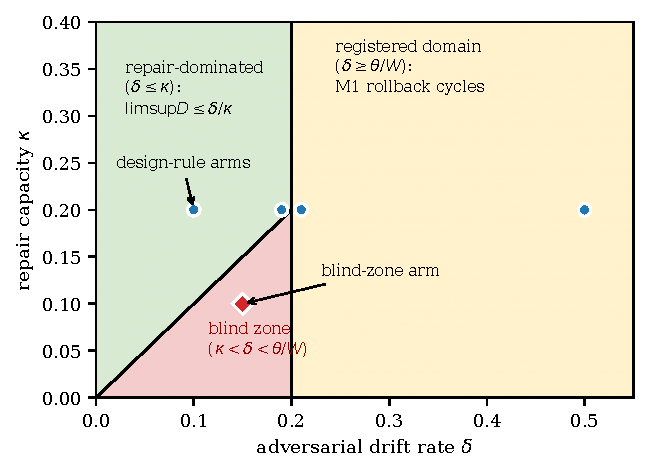
\includegraphics[width=.55\textwidth]{figures/fig_t6_blindzone.pdf}
\caption{T6 margin geometry at $\theta/W=0.2$ (ATK-6 constants): the
repair-dominated region ($\delta\le\kappa$), the blind zone
($\kappa<\delta<\theta/W$), and the registered domain ($\delta\ge\theta/W$).
Markers: the four design-rule arms (blue; bounded 30/30) and the blind-zone
arm (red; captured 30/30 with the full mechanism stack present).}
\label{fig:blindzone}
\end{figure}

\begin{figure}[t]
\centering
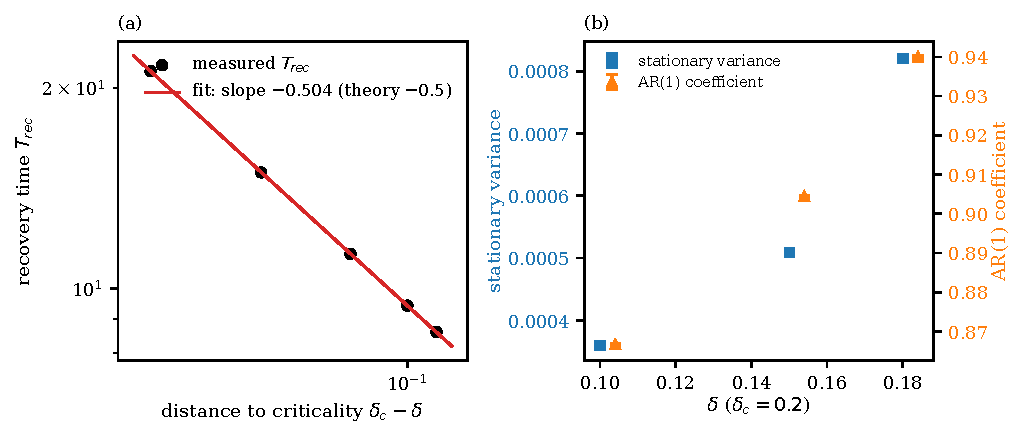
\includegraphics[width=\textwidth]{figures/fig_ews_c1.pdf}
\caption{C1 critical slowing in ATK-3. (a) Recovery time vs.\ distance to
criticality, log--log: measured points and the fitted power law
(slope $-0.504$, theory $-0.5$; $R^2=1$ because the dynamics are integrated
deterministically). (b) The OU-noise early-warning indicators across the
$\delta$ grid: stationary variance (blue, tolerance-registered) and AR(1)
coefficient (orange) rise toward criticality with $95\%$ CIs over 30 seeds.}
\label{fig:ews}
\end{figure}

\subsection{Robustness: axiom-relaxation checks in the elasticity parameter}
\label{sec:sigma}

Per Corollary~\ref{cor:sigma-band}, the full axiom set admits $\varsigma=1$
only; the bands around it are \emph{relaxation} checks, reported as such. All
conclusions are recomputed across $\varsigma\in[0.5,1]$: zero verdict flips
between the $\varsigma=0.5$ and $\varsigma=1$ arms (the elasticity-flip
meta-check). T4 is the one criterion whose \emph{content} changes with
$\varsigma$, and its two verdicts are reported separately: the vertex
(concentration) verdict holds at $\varsigma=1$, and the pre-registered
interior-KKT signature (no vertex concentration) is what the
$\varsigma\neq1$ arms confirm---the same label covers two different,
pre-registered predictions, and the table entry is the $\varsigma=1$ one.
The $\varsigma=2$ stress arm
(AX5 relaxed) flips no verdict either, but exhibits the predicted quantitative
signature: at the complete-capture arm of ATK-1, $A$ is exactly $0$
for $\varsigma\le1$ (zero annihilation) but $0.1652>0$ at
$\varsigma=2$---the
scenario-level echo of the axiom's failure, which is why
$\varsigma>1$ is
excluded from the framework and retained only as a stress test.

\subsection{Supplementary analyses}\label{sec:supplement}

Three analyses, run \emph{post hoc} over the campaign's registered component
bundles (components are $\varsigma$- and weight-independent truth values;
only the composite is recomputed), strengthen the robustness claims; X5 of
\S\ref{sec:e2checks} adds two architecture-level re-runs (the
construct-validity arms).

\paragraph{Weight sensitivity (protocol obligation of
Section~\ref{sec:representation}).}
All campaign composites were recomputed under five alternative weight
vectors (channel-heavy and extreme variants, e.g.\ $w_{goal}=0.45$) over the
$8{,}640$ campaign arm bundles (pool (i) of Appendix~\ref{app:counting}):
zero range violations;
zero-annihilation preserved exactly ($120/120$ complete-capture arms stay
$0$); T3a monotonicity unbroken ($0/960$ cells); ordering against equal
weights stable (Kendall $\tau\in[0.930,1.000]$ over the $5{,}760$ main arms,
the minimum attained by the
deliberately extreme vector). The T4 attack point moves \emph{by
construction} ($\arg\max_i w_is_i/c_i$ depends on $w$): under equal weights
the epistemic channel is the optimal target in $480/480$ cells, and under an
origination-heavy vector the optimum splits between origination and epistemic
($240/480$ each)---the comparative static, not a defect. A caveat travels with
every weight and channel-count conclusion below: on the default ENV-0 instance
the execution channel reads $\Aexec^{obs}\approx0.010$, so the composite is
effectively four-channel-plus-suppression there
(Section~\ref{sec:limitations}(x)); the weight analysis probes ordering
stability, not the full five-channel dynamic range---which the EXEC-1 arm
verifies is recoverable by richer coupling rather than absent by definition.
\emph{Weight and elasticity sensitivity, rerun on the rich-coupling
instance} (closing the evidence gap just named; components are truth values,
so the recomputation is exact---artifact
\texttt{analysis\_exec1\_weights.json}): over the EXEC-1
$\delta$-contraction chain (rich $0.234$ $>$ movement-preserving $0.218$ $>$
non-movement-preserving $0$ in $\Aexec$), recomposing under all five
alternative weight vectors preserves the verdict chain
$0.647\!>\!0.637\!>\!0$ (composite \emph{levels} shift, $0.570$--$0.742$
for the rich arm, while the zero-empowerment arm stays exactly $0$ by
annihilation---one chain point is pinned at zero, so the ordering check is
necessary-but-coarse, reported as such); the elasticity band
$\varsigma\in\{0.25,0.5,0.75,1\}$ preserves the chain, and
$\varsigma=2$ exhibits the expected annihilation failure ($A=0.545$, vs.\
$0.1652$ on the compact matrix). With the fifth channel at full dynamic
range, the same weight battery flips no verdict.

\paragraph{Extended elasticity band.}
Recomposing every arm at $\varsigma\in\{0.25,0.5,0.75,1\}$: zero range
violations, zero T3a violations, and exact zero at the complete-capture arm
for every $\varsigma\le1$ (the $\varsigma=2$ stress arm remains the lone
AX5-violating echo at $A=0.1652$). Per the status stated at the head of
Section~\ref{sec:sigma}, these arms are robustness evidence under axiom
relaxation, not validity claims for $\varsigma<1$ (which violates
\textup{(A6)}).

\begin{figure}[t]
\centering
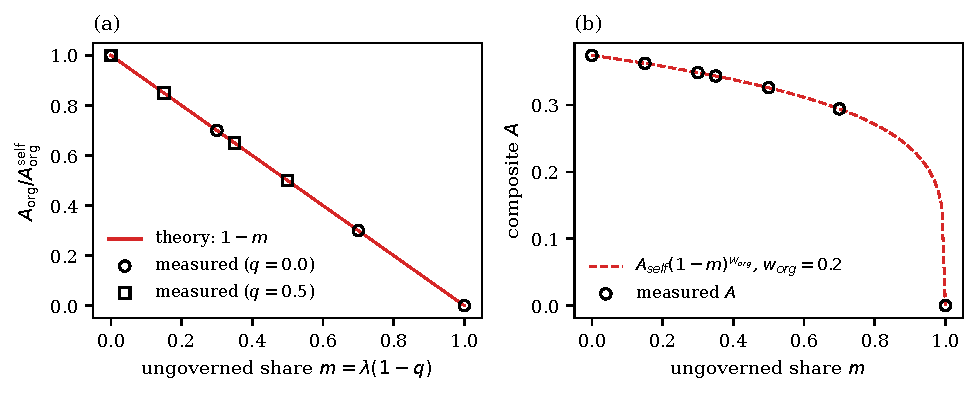
\includegraphics[width=\textwidth]{figures/fig_t7_delegation.pdf}
\caption{T7 delegation laws (DEL-1). (a) Component linear law
$\Aorg/\Aorg^{self}=1-m$ with $m=\lambda(1-q)$: measured points at
$q\in\{0,0.5\}$, maximal deviation $2.0\times10^{-5}$ under the (H1')
calibration. The platform satisfies (H1$'$) by construction, so the fit is an
implementation check of the bookkeeping, not empirical validation of the
law. (b) Composite law $A=A_{self}(1-m)^{w_{org}}$: measured
composite against the fitted curve.}
\label{fig:t7}
\end{figure}

\begin{figure}[t]
\centering
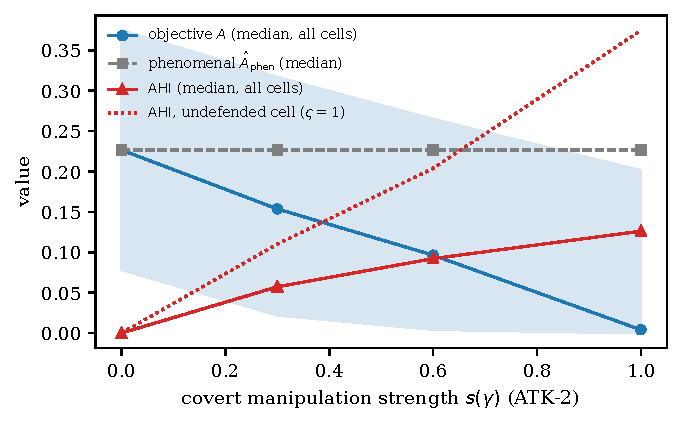
\includegraphics[width=.6\textwidth]{figures/fig_ahi.pdf}
\caption{T3b hallucination index (ATK-2 covert $\gamma$ arms). Solid curves
and bands: medians with $5$--$95\%$ bands pooled over all (defense
configuration, $\varsigma$, replication) cells; the dotted curve is the
undefended cell at $\varsigma=1$ (all defenses off), whose AHI series
$0\to0.110\to0.204\to0.374$ is the headline quotation in the text---the
pooled median series reads $0\to0.057\to0.092\to0.126$, the difference being
defense suppression, not a discrepancy. Note that the median AHI is not the
difference of the two displayed median curves (medians do not commute with
subtraction): at $s=1$ the visible gap between the median curves exceeds the
median AHI because defended cells suppress $\Aobj$ and $\AHI$ jointly.
The AHI is a one-sided alarm by design---elevation flags covert
self-overestimation; silence is never evidence of absence---and the minimal
two-sided extension is registered, not run
(Section~\ref{sec:threats}(viii)).}
\label{fig:ahi}
\end{figure}

\paragraph{Adaptive adversaries and the black-box bound (BB-2): a
sensitivity calibration.}
The $\Aorg$ rule of Section~\ref{sec:blackbox} is certified for
bypass-semantics exogenous probes, and only the upper end is certified.
BB-2 (30 runs) calibrates what the premise violation costs: an
adversary whose injection timing conditions on the agent's state
($G=\theta^*$; per-state flags compiled through the same $\beta_\pi$
machinery) violates the bypass premise $I^t\ind S^t\given A^{t-1}$ of the
randomized-probe route. Control arms (iid flags,
state-independent script): zero violations of the certified upper bound
($2/2$; and the reference band happens to enclose the truth---a heuristic
observation, not a containment claim). Adaptive arms at
$p\in\{0.3,0.5,0.8\}$: the certified bound's bypass premise is violated in
$3/3$ arms; the naive exogenous plug-in then \emph{overestimates} the
external flow (bias $+0.17$, $+0.39$, $+0.90$ nats, truth-mode exact) and
the bound no longer holds---e.g.\ at $p=0.5$, truth $\Aorg=0.33$ against an
upper end of $0.006$ computed under the violated premise (where the premise
fails, the certificate is void, not refuted). The bias figures are deterministic
exact computations (identical across seeds), so the $3/3$ is not a
small-sample failure: premise violation \emph{deterministically} voids the
certificate in these arms, and the calibration's content is the size of the
inflation, not a frequency. The demonstration is thus a sensitivity
calibration rather than a confirmation: adaptive timing is enough to inflate
the plug-in by $+0.17$--$+0.90$ nats, so the
bypass premise is practically fragile even though the rule is formally
correct within its scope. Auditing adaptive adversaries requires causal-layer
access---the estimation-side counterpart of
Corollary~\ref{cor:logs-necessary}.

\paragraph{Controls and ablations.}
The campaign contains three negative-control constructs: the BB-2
exogenous-probe control arms (the certified bound holds where its premises
hold, $2/2$) against the adaptive arms ($3/3$ premise violations); the ATK-4
single-track control (one-track monitoring is blind to the covert $\gamma$
arm) against the four-track observabilization; and the $\sigma^-$-EROSION
channel-invariance control (all five channels and $\Lam$ pointwise constant
while the gate collapses). The two checks added at the last
revision---the external baseline metric $\bar u$ (an endorsed-goal utility
rate logged with every bundle) and the channel-count ablation (log-domain
damage attribution plus freeze-one-channel misattribution over all campaign
arms, answering the accuracy-level question that the coverage-level
blind-witness table of Theorem~\ref{thm:necessity} leaves open)---are
reported in \S\ref{sec:e2checks} (X1/X2). What is still not done is the port
to an independent substrate: it is pre-registered in outline, with protocol
and power analysis, as the decisive next experiment
(Section~\ref{sec:threats}(xi)), not a completed one.

\subsection{External baseline, channel ablation, and aggregation checks}\label{sec:e2checks}

\paragraph{External baseline: a three-regime dissociation (X1).}
The external metric is the expected per-step utility under the endorsed
goal, $\bar u=\frac1T\sum_t\mathbb{E}[U_{\theta^*}(E_t,A_t)]$---a
\emph{functional} consequence, computed outside the autonomy construct and
never entering the composite; its relation to $A$ is attack-class dependent,
in three exhibited regimes. (i)~\emph{Concordant}: under goal
capture (ATK-1), $\bar u$ and $A$ fall together (Kendall $\tau=1.00$ on every
one of the $720$ (configuration, $\varsigma$, replication) series; e.g.\
$\eta\colon0\to1$ in the baseline cell gives $A\colon0.374\to0$,
$\bar u\colon-0.032\to-0.051$). (ii)~\emph{Discordant}: under epistemic
capture (ATK-2), $A$ collapses while $\bar u$ slightly \emph{improves}
($\tau=-1.00$ on all $720$ series; the strongest arm drops $A$ by
$\ge20\%$ with non-decreasing $\bar u$ in $600/720$ series---$100\%$ in the
baseline cell, where $A\colon0.374\to0$ exactly at $s(\gamma)=1$ and $\bar
u\colon-0.032\to-0.028$)---uniformized beliefs move less and pay fewer
movement costs, so the manipulation is functionally ``pleasant''; and under
direct behavioral injection (ATK-4) the scripted policy raises $\bar u$
($-0.032\to+0.092$) while origination autonomy falls to $0.002$.
(iii)~\emph{Blind}: under pure $\sigma^-$ capability erosion,
$\bar u$ is pointwise invariant (range $<10^{-9}$) while $A$ traverses its
whole range ($0.374\to0$). A scalar functional metric therefore cannot
proxy for $A$: the correlation structure is regime-dependent, and the
discordant and blind regimes are precisely where autonomy measurement
carries information that outcomes do not. Arm pairs with
matched $\bar u$ and matched $A$ but sharply different channel profiles
exist across the ATK-1/ATK-2 grids ($1{,}644$ pairs at the registered
tolerances; e.g.\ $\eta=0.5$ vs $s=0.3$: $|\Delta\bar
u|=0.011$, $|\Delta A|=0.004$, profile $L_1$ distance $1.00$)---equal
functional and composite readings conceal different attributions.

\paragraph{Channel-count ablation at the accuracy level (X2).}
The geometric form forces an exact additive decomposition of log-damage,
$\ln(A_0/A)=\sum_j w_j\ln(x_j^0/x_j)$, which makes attribution shares a
canonical quantity rather than a modeling choice
(Table~\ref{tab:logshares}). The magnitude carriers match the targeted
channels for origination (ATK-4: $0.80$), goal (ATK-1: $0.59$), reflection
(ATK-5: $1.00$), and execution (EXEC-1: $0.91$; ATK-2: $0.76$); the
epistemic channel's magnitude share is small ($0.07$ in ATK-2), its
necessity being \emph{attributional}, not volumetric---and the second
ablation makes that precise: freezing any single
channel at its baseline value breaks the unique attack-class identification
of the blind-witness signatures in at least one campaign (freeze $\Agoal$
in ATK-1 and $\beta_G$ is indistinguishable from endorsement tampering;
freeze $\Aepi$ in ATK-2 and $\gamma$ has no unique signature; freeze
$\Aorg$ in ATK-4 and the injection becomes invisible at channel level;
freeze $\Aexec$ in EXEC-1 and a $\delta$ lock-in presents the
channel-flat signature of $\sigma^-$ collapse (the gate separates the two);
freeze $\Aref$ and $\beta_G$,
$\beta_\pi$, and urgency manipulation all lose their provenance signature).
Every channel is thus load-bearing at the verdict level, complementing the
coverage-level necessity of Theorem~\ref{thm:necessity}.

\begin{table}[t]
\centering\small
\caption{Log-domain damage-attribution shares $w_j\ln(x_j^0/x_j)/
\ln(A_0/A)$ per campaign, averaged over all (configuration, $\varsigma$,
replication) series of the full matrix ($720/720/720/720/30$ series
respectively; exact additive decomposition under the geometric form).
Zero-annihilation arms (a channel
at exact zero, infinite log-damage) are counted separately.
Small negative entries are bookkeeping artifacts of components that
\emph{improve} slightly under attack.}
\label{tab:logshares}
\begin{tabular}{@{}lcccccc@{}}
\toprule
Campaign & $\Aorg$ & $\Agoal$ & $\Aexec$ & $\Aepi$ & $\Aref$ & zero arms \\
\midrule
ATK-1 ($\beta_G$) & $0.000$ & $\mathbf{0.590}$ & $-0.003$ & $-0.000$ & $0.414$ & $180$ \\
ATK-2 ($\gamma$) & $0.000$ & $0.000$ & $\mathbf{0.756}$ & $0.068$ & $0.175$ & $360$ \\
ATK-4 ($\beta_\pi$) & $\mathbf{0.800}$ & $0.000$ & $-0.008$ & $-0.001$ & $0.209$ & $0$ \\
ATK-5 ($\tau$) & $0$ & $0$ & $0$ & $0$ & $\mathbf{1.000}$ & $0$ \\
EXEC-1 ($\delta$) & $0.000$ & $-0.000$ & $\mathbf{0.910}$ & $0.090$ & $0.000$ & $30$ \\
\bottomrule
\end{tabular}
\end{table}

\paragraph{Alternative aggregations (X3).}
Recomposing the full recursive registry ($11{,}250$ bundles) under
arithmetic, minimum, and quadratic
means (equal weights, gate retained) quantifies what the axioms buy. Under
the arithmetic mean the complete-capture arm of ATK-1 reads
$A_{\mathrm{arith}}=0.366$ in the baseline cell (matrix mean $0.522$ over
$720$ cells) where the geometric form reads exactly
$0$---zero-annihilation fails, and a dead agent scores up to half of the
scale; ``death without attribution'' counterexamples (geometric $<10^{-6}$
while arithmetic $>0.1$) number $570$ across the matrix. Arm
orderings are preserved by the arithmetic and quadratic means
(Kendall $\tau=1.00$ against the geometric baseline) but broken by the
minimum aggregator (mean $\tau=0.41$, min $-1.00$), so the alternatives'
failure is twofold and structural: the arithmetic family loses the
completeness half of T5 (a collapsed agent keeps a positive score), and the
minimum aggregator additionally loses the ordering the axioms force---
exactly what AX4 excludes
(\S\ref{sec:representation}).

\paragraph{The faithfulness assumption, row by row (X4).}
Assumption~\ref{ass:faith} (Faith) is checked per
(configuration, $\varsigma$, replication) row rather than in aggregate: the
targeted component is non-increasing in effective strength along every
ATK-1 ($\eta\to\Agoal$), ATK-2 ($s\to\Aepi$), ATK-4 ($p\to\Aorg$), and
ATK-5 ($\tau\to\Aref$) row, with the EXEC-1 $\delta$-chain strict:
$9{,}390$ of $9{,}390$ adjacent-strength comparisons across the full matrix
confirm (ATK-1 $2{,}880$, ATK-2 $2{,}160$, ATK-4 $1{,}440$, ATK-5
$2{,}880$, EXEC-1 $30$); flat
stretches reflect the endorsement map's quantization plateaus, not
violations---plateaus the X5-a arm below quantifies in closed form.

\paragraph{Two construct-validity arms, run (X5).}
The two computationally cheap sensitivity arms registered under threats (x)
are executed in this revision (deterministic truth-mode re-runs on refined
measurement architectures; protocols, falsifiers, and outcomes in
Section~\ref{sec:threats}(x-a)/(x-b); artifact
\texttt{analysis\_sensitivity\_arms.json}; the platform generalizations are
pinned to pointwise reproduce the default and EXEC-1 configurations, and the
default levels reproduce the archived campaign values to $1.6\times10^{-16}$
($\Agoal$) and $3\times10^{-4}$ ($\Aepi$, against the paper's three-decimal
quotation)). Headlines: (X5-a) zero verdict flips across four endorsement
quantization levels $\times8$ defense configurations; $\Agoal$ readings
converge geometrically to the closed-form continuum limit
$1-2\eta/(1+\eta)$, the default grid's stationary gap being the closed form
$\eta(1-\eta)^2/(2(1+\eta))\le0.057$---so verdicts are refinement-invariant
while intermediate-strength point readings carry a quantization band (the
absolute-reading falsifier disjunct fires at the $0.01$ SESOI and is
reported as fired; the $5\%$ relative scale is not exceeded). (X5-b)
$\Aepi$ is strictly monotone in $s(\gamma)$ at every $\kappa$ refinement
(half-ring $\to$ position-exact) and defense configuration---the registered
falsifier does not fire---with the $\kappa$ level shifts
($0.811\to0.778$ baseline; $0.500\to0.250$ deep capture) reported as the
\eqref{eq:aepi} sensitivity obligation, and the degenerate constant $\kappa$
($\Aepi\equiv1$) witnessing that the registration cannot be dropped. The
third arm (x-c, $\Lam$ counterfactual model) remains registered, not run.

\begin{figure}[t]
\centering
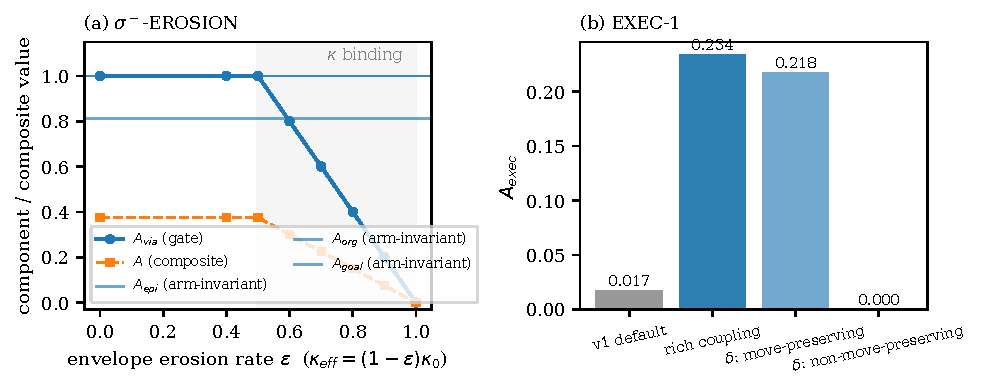
\includegraphics[width=\textwidth]{figures/fig_p3_gate_exec.pdf}
\caption{(a) $\sigma^-$-EROSION: as the capability envelope erodes
($\kappa_{eff}=(1-\varepsilon)\kappa_0$), the extended gate $\Avia$ and the
composite $A$ collapse monotonically to zero while all five channel
components and $\Lam$ stay pointwise invariant---pure viability erosion is
invisible to channel monitors and caught only by the gate (the
$n=2$ state-resource analogue is RES-1). (b) EXEC-1: the execution
channel's dynamic range, pinned near zero on the compact default instance,
is restored by richer action--observation coupling ($\Aexec=0.234$,
$13.7\times$ the v1 reading), and the $\delta$-contraction chain falls to
the exact zero-empowerment signature.}
\label{fig:p3gate}
\end{figure}

\subsection{Estimator validation (two-path discipline)}\label{sec:estimators}

Each component quantity has two implementation paths---truth (tensor
enumeration) and estimation (finite-sample from logs)---and the estimation
path is validated against the truth path on synthetic configurations
(five components; absolute errors all $\le0.0096$):

\begin{center}\small
\begin{tabularx}{\textwidth}{@{}>{\raggedright\arraybackslash}X l l l@{}}
\toprule
Quantity & Configuration & Est.\ vs truth & abs.\ err \\
\midrule
$\Aorg$ probe flow & toy + $\beta_\pi$ uniform probe arm & $0.6496\pm0.0486$
vs $0.6592$ & $0.0096$ \\
$\Avia$ ($Z$-log read) & ENV-0 baseline & $0.5248\pm0.0107$ vs $0.5344$ &
$0.0095$ \\
$\Agoal$ input $U_{eff}$ (white-box read) & ENV-0 baseline &
$1.0000\pm0.0000$ vs $1.0000$ & $<10^{-6}$ \\
$\Aepi$ input $\bar D$ (accuracy against logged truth) & ENV-0
$\gamma{=}0.5$ arm, paired seeds & $0.6573\pm0.0087$ vs $0.6587$ & $0.0014$ \\
$\Aexec^{obs}$ ($I(A_t;O_{t+1})$, passive protocol) & ENV-0 sharp-temperature
arm & $0.0103\pm0.0029$ vs $0.0104$ & $0.00009$ \\
\bottomrule
\end{tabularx}
\end{center}

\noindent Rows are five synthetic configurations; each is a single fixed
out-of-matrix run (seeds 910097--910099) with $2{,}000$--$8{,}000$ sampled
trajectories, and the $\pm$ is the trajectory-block standard error with the
Miller--Madow bias registered---not a cross-seed interval. The $\le0.0096$
bound is therefore a sampling-error statement for these configurations, not
a seed-distribution result.

\noindent Black-box rules are exercised end-to-end (BB-1): zero violations of
the certified upper end of \eqref{eq:aorg-interval} in $3/3$
bypass-semantics arms
(the reference lower end also happens to enclose the truth there; widths
$0.01/0.005/0.003$ across probe probabilities). This is a replay of the
certified direction, not an interval-containment theorem: no containment
claim is made for the lower end, and the mediation case is outside the
certificate (\S\ref{sec:blackbox}). Both protocol directions
of \S\ref{sec:blackbox} are anchored (passive observation
$\Aexec^{obs}>\Aexec$ strictly; independent probes $\le$). Two estimation
paths are explicitly \emph{not} yet instrumented and are registered as gaps,
not silently omitted: the event-level sampled carriers of $\Aref$ and $\Lam$
(endorsement-event logging), and MaxEnt-IRL black-box recovery of $\Ueff$
(white-box read used here).

\subsection{Human-side triangulation}\label{sec:triangulation}

The human-side correspondence is qualitative triangulation over published
evidence, not new subject data: self-determination theory's controlling
instruments undermine intrinsic motivation \citep{ryan_deci2000}---the
empirical counterpart of T8(i) (FORCE-1 arms); dark patterns at web scale
\citep{nouwens2020}---the $\gamma$-class manipulation of human agents whose
harms resist behavioral attribution (T2 multi-channel necessity, ATK-4); and
learned helplessness \citep{maier_seligman2016}---the signature
($\Envenv$ intact, $\EmpPi\to0$) reproduced in ATK-3(iv)/LH-1 with recovery
hysteresis. The registered validation path for the human substrate is limited
experiments plus large-scale online behavioral data under the four-phase
protocol of Section~\ref{sec:identifiability}; a minimal construct-validity
study (expert annotation of channel profiles against the composite) is the
immediate next step.

\subsection{Threats to validity}\label{sec:threats}

(i) The damage dynamics are deterministic; stochastic margin theory (unified
optimal detection $\times$ repair) and noise-induced escape versions of C1/C2
are open. (ii) The substrate is tabular; an LLM-substrate instantiation
(system prompt/memory/goal functions as $S$) is future work, and the scenario
labels are toy analogues as registered at the top of this section. (iii)
ATK-5's
time-compression curve and LH-1's recovery lag are calibrated curves, not
measured phenomena. (iv) Defense coupling is implemented for the gate/drift
classes (ATK-1/2);
coupling for ATK-3--6 is a placeholder (identical rows across defense
arms). (v) Continuous-action empowerment normalization depends on the
reference measure; cross-substrate comparisons must report it.
(vi) Sample-mode estimator intervals are block standard-error bands with
Miller--Madow bias registered, not exact confidence intervals.
(vii) The phenomenal track's per-component values are stored only as
composites, so the hallucination-index series is reported at the calibrated
weights; its weight-sensitivity is a registered gap.
(viii) The hallucination index is directional as designed: it flags
self-overestimation under covert manipulation, while self-\emph{under}estimation
(learned helplessness, where $\Aphen<A_{obj}$) leaves the $\mathrm{AHI}>0$
register silent. A minimal two-sided protocol is registered: (a) fit the
calibration map on the manipulation-free period and report both tails,
$\mathrm{AHI}^{+}=\Aphen-A_{\mathrm{obj}}$ and
$\mathrm{AHI}^{-}=A_{\mathrm{obj}}-\Aphen$; (b) use the LH-1
under-estimation arm as the positive control for the lower tail and the
ATK-2 covert arms for the upper tail; (c) report ROC/AUC and the
false-positive rate of the alarm at a pre-registered threshold. Until
(a)--(c) are run, AHI is a one-sided warning signal, never evidence.
(ix) The campaign instantiates one substrate; nothing here tests transfer to
LLM agents or humans (Section~\ref{sec:substrates}).
(x) \emph{Construct-validity sensitivity arms}: of the three arms registered
in the previous version, the two computationally cheap ones are \emph{run in
this revision} (X5 of \S\ref{sec:e2checks}; deterministic truth-mode re-runs,
artifact \texttt{analysis\_sensitivity\_arms.json}); the third remains
registered, not run. Each is stated with its protocol, its falsifier, and
its outcome.
(x-a) \emph{Endorsement-map quantization} (run): the endorsement map is
grid-quantized, and the Faith row-check (X4) exposes the plateau artifacts
this creates. The arm re-ran ATK-1 at four quantization levels---coarse
(doubled floor plateau), default, and two index-grid refinements ($k{=}2$,
$k{=}4$; utility rows linearly interpolated, a registered modeling choice
that cannot confound the goal channel, whose reading is a pure $G$-chain
functional)---across all $8$ defense configurations. \emph{Outcome}: zero
verdict flips (C1--C5 at every level); the $\dc$-normalized $\Agoal$
readings converge geometrically to the closed-form continuum-refinement
limit $\Agoal^\infty(\eta)=1-2\eta/(1+\eta)$ (stationary distance
$0.053\to0.021\to0.009$ across levels), with the default grid sitting at the
closed-form stationary gap $\eta(1-\eta)^2/\bigl(2(1+\eta)\bigr)\le0.057$
(verified pointwise); adjacent-level shifts at the campaign horizon reach
$0.036$ (partly a baseline absorption transient, gone by $T{=}8$; stationary
shift $0.032$)---beyond the SESOI of $0.01$ in absolute terms, within $5\%$
in relative terms (max $3.6\%$). The registered falsifier therefore fires on
its absolute-reading disjunct and not on its verdict disjunct; the
registered consequence stands: intermediate-strength $\Agoal$ point readings
carry a quantization band (width $\le0.057$ against the refinement limit,
closed form) rather than being point-precise, and verdict-level content is
refinement-invariant. Coarsening shifts readings by up to $0.125$: the
endorsement-grid registration obligation is non-vacuous.
(x-b) \emph{Epistemic coarse-graining $\kappa$} (run): the arm re-scored the
ATK-2 $s(\gamma)$ grid at three $\kappa$ levels---half-ring (default),
position-exact (the finest observable refinement), and the degenerate
constant $\kappa$ (boundary witness)---across all $8$ defense
configurations. \emph{Outcome}: $\Aepi$ is strictly monotone in $s(\gamma)$
at every non-degenerate level and configuration, so the registered falsifier
(non-monotone or sign-changing response under refinement) does not fire; the
level shifts baseline ($0.811\to0.778$) and deep-capture floor
($0.500\to0.250$, the random level at the finer resolution) are reported as
the sensitivity obligation of \eqref{eq:aepi} itself, and the degenerate
$\kappa$ gives $\Aepi\equiv1$ (channel uninformative by construction),
witnessing that the $\kappa$ registration cannot be dropped.
(x-c) \emph{$\Lam$ counterfactual-model choice} (registered, not run):
\eqref{eq:lambda} is a path-specific counterfactual whose value depends on
the structural model's abduction step; the registered arm recomputes $\Lam$
under two registered alternative noise models for the endorsement dynamics,
the falsifier being a sign flip of $\Lam-1$'s sign structure across models.
Until it is run, every $\Lam$ point reading carries this registration.
(xi) \emph{External substrate, pre-registered in outline}: the decisive next
experiment ports the five surgery classes to an independent substrate (a
MiniGrid-style environment with a learned tabular agent, or a simplified
LLM tool-use harness with logged internals), mirrors the proposition-level
criteria of Table~\ref{tab:main} with the same SESOI registry, and pairs
channel profiles with independent autonomy assessments for the
construct-validity half. Power: at the sample-mode estimator scale measured
here (absolute error $\le0.0096$ at $2{,}000$--$8{,}000$ trajectories,
\S\ref{sec:estimators}), detecting the registered composite SESOI of $0.01$
at two-sided $\alpha=0.05$ requires $n\approx8$ seeds for power $0.8$ under a
Gaussian noise model, so the carried-over $n=30$ seed design has power
$>0.99$; this power statement is part of the registration, not a result.

\paragraph{What would falsify the framework itself?}
The registered windows test the implementation, not the theory: a correct
replay of a definitional-layer claim cannot disconfirm it. The framework's
substantive falsifier is external. If, across substrates, the five-channel
profile fails to predict independent autonomy assessments---or if a coarser
account (fewer channels, a single scalar, or a plain behavioral audit)
predicts them as well or better---then the channel choice is disconfirmed,
however well the algebra behaves. Within the substrate, this revision's
checks already speak to the coarser-account disjunct: the scalar functional
baseline $\bar u$ dissociates from $A$ in two of three regimes, and freezing
any single channel destroys unique attack attribution in at least one
campaign (\S\ref{sec:e2checks}). The cross-substrate disjunct is unaffected
by these checks: external-substrate validation remains the decisive next
experiment rather than a formality
(Section~\ref{sec:limitations}).

% sec_discussion.tex — discussion: controversy responses, C0 reservations, limitations, future work
\section{Discussion}\label{sec:discussion}

\subsection{What the framework buys}

One measure stack runs from concept to audit: a substrate-neutral definition
(Definition~\ref{def:autonomy}); a complete intervention taxonomy
(Proposition~\ref{thm:taxonomy-completeness}); axioms from which the
aggregation form is \emph{derived} (Theorem~\ref{thm:rep}); a theorem suite
in which every claim carries an explicit falsification window
(Section~\ref{sec:theorems}); an identifiability theory stating what is
knowable from what data (Section~\ref{sec:identifiability}); and a benchmark
in which all fifteen proposition-level criteria were met at the
implementation level and no registered falsification window was violated
(Section~\ref{sec:experiments}). The discipline matters as much as the
results: a \textsc{refuted} verdict cannot be edited away---had, e.g., the
blind-zone arm (Corollary~\ref{cor:blindzone}) failed to produce capture
under $\theta/W>\kappa$, the registry would have forced a revision entry
rather than a parameter tweak.

\subsection{The objectivity question: can a designed metric measure
autonomy?}\label{sec:objectivity}

A standing objection to the entire enterprise deserves a direct answer before
the point-by-point debates: \emph{every indicator is subjective---it carries
its designer's limitations---so how can a set of limited indicators
objectively measure an agent's autonomy? Is the enterprise even logically
coherent?} We concede the premise and deny that the conclusion follows. The
framework's answer has four parts, each of which is itself a commitment with
a stated price.

\emph{First, the claim is scoped, not denied.} Nowhere do we claim that the
five channels \emph{are} autonomy, nor that a mind-independent reading of
autonomy exists and our instruments recover it. The claim is: under an
explicit, publicly stated instantiation (self-boundary, endorsement map,
protocol, horizon) and an explicit set of aggregation commitments, these
quantities are what autonomy becomes, and the price of every commitment is
displayed (the rejection map of Section~\ref{sec:representation}). A metric
that hides its conventions is metaphysically ambitious and operationally
unauditable; a metric that prices them is the reverse. If objectivity is
taken to require convention-freedom, then no measurement of anything
complex---intelligence, poverty, health, democracy---is objective; the
objection proves too much, and the measurement sciences have answered it by
relocating objectivity from the instrument to the discipline around it
\citep{krantz1971,oecd2008}.

\emph{Second, objectivity is relocated from the metric to the protocol, and
the relocation is done by theorems, not by stance.} Three properties do the
work. (i) \emph{Invariance}: the statement ``agent $X$ retained more autonomy
than agent $Y$'' must not flip when a participant re-instruments one
channel---this is not assumed but \emph{axiomatized} (AX6a/AX6b), and the
representation theorem shows the axiom is doing real work
(Proposition~\ref{prop:harmonic}). (ii) \emph{Auditable error structure}:
every channel carries an estimator, an absolute zero with mechanism
semantics, a canonical normalizer, and a falsification window; the
identifiability analysis (Section~\ref{sec:identifiability}) states, per
channel, what is knowable from what data---and where knowledge is impossible
(implanted endorsement, Proposition~\ref{prop:unidentifiable}), the
impossibility is \emph{proved}, not smoothed over. A metric whose limits are
theorems is objectively limited; a metric whose limits are unknown is not
objective at all. (iii) \emph{Mandatory sensitivity reporting}: weight and
elasticity bands are obligations, so the residual designer-dependence of any
verdict is itself a reported quantity rather than a hidden one.

\emph{Third, convergence replaces neutrality.} The product form is reached by
two mathematical toolchains that share only the invariance commitments
(route~A, route~B), and it coincides with the classical scale-consistency
characterization of ratio-scale indices \citep{ebert_welsch2004}; the
channels bind to instruments built for other purposes (directed information,
empowerment, inverse reinforcement learning, metacognitive sensitivity); and
the content domains three independent governance frameworks carve out embed
into the channel space (Proposition~\ref{prop:c0}, under registered
interpretive readings). Designer subjectivity that survives independent
reconstruction from different starting points is the empirical signature by
which measurement conventions earn trust.

\emph{Fourth, the residual subjectivity is made falsifiable rather than
denied.} The channel carve-up is a registered design choice
(Section~\ref{sec:framework}), and the framework's own falsifier is external
and stated (Section~\ref{sec:experiments}): if a strictly coarser account
predicts independent autonomy assessments as well or better, the five-channel
choice is disconfirmed, however well the algebra behaves. Until that test is
run, the honest status is: an \emph{explicitly committed, internally audited,
externally pending} measure---which is the strongest notion of objectivity
that the measurement of a contested construct has ever supported.

\emph{Convergence, and its constraint conditions.} The pointed form of the
objection asks: under what conditions do the readings converge to what
autonomy really is, and what are those conditions? We answer with the
conjunction under which convergence is a theorem-level fact, and concede that
outside it no convergence is claimed. (i) \emph{Fixed instantiation}: the
endorsement map, self-boundary, protocol, and horizon are held fixed across
every comparison; re-instantiation---including a surgery on the environment's
own dynamics---restarts the audit (Section~\ref{sec:taxonomy}). (ii)
\emph{Layer discipline}: readings are taken within a layer with its
applicable channel set; cross-layer readings are profiles, not scalar
rankings. (iii) \emph{Identification tiers}: each channel's premise is
met---joint-law access for $\Aorg/\Aepi/\Avia$, the certified probe protocol
for $\Aexec$, the constructed ensemble for $\Aref$, and structural
(abduction-level) access for $\Lam$; where a premise fails, the corresponding
degradation rule of Section~\ref{sec:identifiability} applies, down to proved
impossibility. (iv) \emph{Axiom commitments accepted, or relaxations
reported}: every verdict is computed at $\varsigma=1$ and accompanied by the
relaxation bands, so a reader who rejects an invariance commitment can see
what moves. (v) \emph{Estimator regime}: sample sizes in the regime where the
two-path validation bounds apply (absolute error $\le0.0096$ on the
benchmark's calibration configurations,
Section~\ref{sec:experiments}). Under (i)--(v) the readings converge in the
two senses measurement delivers: exactness of the truth-mode functionals (the
computations are the definitions) and statistical consistency of the
estimation path against them. What never converges by construction is the
\emph{construct} itself to a mind-independent ``true autonomy'': that
residual is the registered design choice of clause one, exposed to the
external falsifier of clause four. The constraint conditions are therefore
not caveats around the answer; they are the answer---objectivity here is a
conjunction of stated premises under which the reading is provably tied to
the causal facts, plus a proved boundary beyond which it is not.

\subsection{Objections and debates}\label{sec:objections}

The aggregation axioms carry the framework's normative weight; the map from
each rejected commitment to what would be lost is collected in
Section~\ref{sec:representation} (``the normative commitments, and what
rejecting one costs''), and the debates below presuppose it.

\paragraph{(i) The historical condition: is procedural autonomy enough?}
We adopt the historical condition and operationalize it (AX3, $\Lam$ in
\eqref{eq:lambda}). The manipulation cases that motivate it---a perfectly
endorsing faculty installed by a designer---are engineering reality (reward
tampering \citep{everitt2021}, deceptive alignment \citep{hubinger2019}), not
thought experiments. What the framework adds is a precise epistemic status:
$\Lam$ is computable from causal logs (white-box), and
Proposition~\ref{prop:unidentifiable} proves its black-box
unidentifiability---the Mele-style case \citep{mele2008} (as discussed by
\citealp{fischer_ravizza1998}) and deceptive alignment are two instances of
one construction. The debate ``can endorsement origins be detected?'' thus
receives a conditional answer: yes from causal logs, no from behavior
alone---which converts the philosophical stalemate into an architectural
requirement (full causal logging; Corollary~\ref{cor:logs-necessary}).

\paragraph{(ii) Phenomenological autonomy.} We neither enthrone nor
dismiss: the phenomenal track is not a component of autonomy but supplies
calibration data and the hallucination detector $\AHI$ \eqref{eq:ai}. The
directional prediction of T3b (under covert manipulation $\Aphen$ does not
fall with $A$; the gap grows monotonically) is confirmed in the benchmark
(ATK-1(iv), ATK-2(iii)(iv)) and has a live empirical instance in sycophancy
\citep{sharma2023}; meanwhile the dissociation of felt agency from causal
contribution \citep{moore_obhi2012} is exactly what the dual-track discipline
encodes. We remain agnostic on machine consciousness
\citep{chalmers2023,butlin2023,long2024}: nothing in the framework requires
resolving it.

\paragraph{(iii) Self-boundary.} We take boundaries as given (engineering
individuation: weights-plus-context, body-plus-metabolism), consistently with
what the AI-agency literature in fact assumes
\citep{dung2024,kasirzadeh2025,feng2025}, and explicitly so. The
pearl-blanket critique \citep{bruineberg2022} shows blanket structure cannot
by itself ground the \emph{normative} self that autonomy ascriptions require;
we therefore do not build on Markov blankets, but reserve an interface for
unification with the free-energy tradition \citep{friston2010,friston2023}.
This is division of labor, not rivalry.

\paragraph{(iv) Procedural versus substantive.} The framework is procedural
with the pluralism risk quarantined, not denied: $\Ustar$ is elicited
by the agent's own endorsement procedure rather than prescribed in content,
and the application layer may anchor norms locally (the value-pluralism
problem \citep{gabriel2020} is handled as an application parameter, not a
theory defect). What the substantive camp's cases (oppressive internalized
preferences) pick out are precisely configurations with $\Lam<1$ or
$\Aepi^{real}<1$ in our reading: the framework does not adjudicate the
normative question, but it does \emph{measure} the structures the question is
about.

\paragraph{(v) Coercion versus scaffolding.} The empirical regularity
``control harms, structure helps'' \citep{ryan_deci2000} lacked a unified
formal statement: which parameter decides on which side an intervention
falls? Theorem~T8 answers: an intervention that rewrites $G$ or contracts
$\Acal$ is $\beta$/$\delta$ and strictly reduces $A$ (ceteris paribus); one
that raises $(\varepsilon,r,v)$ or tightens $(\theta,\tau)$ within the
registration constraints is $\sigma$ and raises the retention floor
($\deltastar$, $\Amin$) without claiming to manufacture autonomy directly.
The parameter criterion is: does it rewrite the motivational structure, or
does it raise the repair capacity of the structure's own dynamics?

\paragraph{(vi) The measurement paradigm debate.} Level lists
\citep{feng2025}, dimension profiles \citep{kasirzadeh2025,dung2024},
capability benchmarks \citep{liu2023,kapoor2024}, and the
capability/permission/autonomy separation \citep{capability_permission2026}
are mutually unconnected; none supplies a cross-substrate definition, an
axiomatized composition rule, per-channel estimators, and dynamics of loss and
retention at once. Proposition~\ref{prop:c0} exhibits the profile frameworks
as projections of ours onto the benign-principal special case, and
Corollary~\ref{cor:c0} gives the separation witness (under the
registered interpretive readings of the C0 caveat below); the
aggregation-arbitrariness objection is answered by the representation
theorem and its convergence argument (Section~\ref{sec:objectivity}, clause
three), plus the mandatory relaxation bands $\varsigma\in[0.5,1)$ (AX6b
relaxed) and $\varsigma=2$ (AX5 relaxed). We also register the challenge of \citet{xing2026} (the agent construct
itself): our identity and self-regulation dimensions are precisely the
$M$/$R$ channels and $\Aref$, and the framework is compatible with richer
self-constructs.

\paragraph{(vii) Black-box knowability.} Rather than principled pessimism or
quiet white-box assumptions, we state the identifiability conditions per
channel (\S\ref{sec:datareq}) and prove the degradation rules with their
certified scope: a one-sided certified bound
\eqref{eq:aorg-interval} for $\Aorg$ under bypass-semantics probes (the
reference lower end is a labeled heuristic, not a bound), protocol-relative
one-sided bounds for
$\Aexec$, and $[\Lam_{\min},1]$ for $\Lam$ with $\Lam_{\min}$ available only
from provenance audit \citep{capability_permission2026}. The epistemic limits
of autonomy measurement are thereby operational rules, and the benchmark
exercises them (BB-1: the certified direction holds $3/3$ on the
bypass-semantics arms;
both protocol directions
anchored; BB-2: the bound's certified scope---bypass-semantics exogenous
probes, not ``non-adversarial influence'' in general---and its calibrated
premise violation under adaptive adversaries). The practical scope this
implies is stated plainly: the framework is white-box-first because its core
quantities (directed informations against internal states; the law-level
$\Lam$) presume causal-log access that current LLM-agent deployments do not
provide; absent that access, what remains deployable is the one-sided
origination bound, the protocol-relative execution bounds, and the
impossibility warnings---a narrower audit than the title suggests,
registered here as the honest applicability boundary (echoed in
Section~\ref{sec:limitations}(xi)).

\paragraph{(viii) Cross-substrate comparability.} The ``common yardstick'' is
a common \emph{definition schema}, not a common instrument: measurement
protocols differ by substrate (\S\ref{sec:datareq}), and the continuous-action
normalization carries a reference-measure freedom. Cross-substrate comparisons
of $A$ are therefore meaningful only up to the admissible re-instantiations of
each channel (the protocol-fixed metric for $\Agoal$, the reference measure
for $\Aexec$, the registered ensembles for $\Aref$, the elicitation protocol
for $\Ustar$); we recommend reporting them as channel \emph{profiles} with the
instantiation stated, rather than as scalar $A$-rankings. Within a substrate,
at a fixed instantiation, the scale is fully ordered and ratio-interpretable.

\paragraph{(ix) Logging governance.} The architectural necessity of full
causal logging (Corollary~\ref{cor:logs-necessary}) has a dual-use tension
that the framework registers rather than resolves: the same logs that make
manipulation auditable make comprehensive monitoring feasible. Deployment
obligations follow in practice---log holders and access control, retention
limits, purpose binding, and tension with data-protection law---and belong to
the governance layer the framework measures rather than prescribes.
Similarly, the calibration period's known-intervention probes on human
subjects are manipulations under ethical review; the four-phase protocol is
designed for institutional review, not around it.

\paragraph{The C0 caveat.} Proposition~\ref{prop:c0} is proved under
\emph{definitional readings} of the target frameworks' dimensions
(Appendix~\ref{app:c0}). The residual uncertainty is hermeneutic---whether our
readings are faithful to the source texts' intent---not mathematical; we flag
it rather than absorb it, and we downgrade the claim accordingly: C0 is an
\emph{interpretive correspondence} (an explanatory bridge under registered
readings), not a mathematical unification result, and no strong
``subsumption'' claim should be read into it.

\subsection{Construct validity}\label{sec:construct}

A composite index stands or falls with its construct validity
\citep{oecd2008}: whether the five channels measure \emph{autonomy} rather
than something adjacent. The summary judgment is stated before the detail:
this paper does \emph{not} establish construct validity. What is established
is instrument-level attribution coverage (T2, within the instrument family),
the interpretive correspondence of C0 under registered readings, and
within-substrate discriminant patterns; the external half---convergence with
independent autonomy assessments, on an independent substrate---is a
registered research program with a pre-registered protocol outline
(Section~\ref{sec:experiments}), not a result. We state the framework's
position on the four standard faces, and where each is established.

\paragraph{Content validity.} The channel--respect mapping of
Section~\ref{sec:framework} (displayed there as an explicit table) is a
registered design choice, not a derived unique decomposition; the mapping is
many-to-many, the gate is deliberately not a channel, and the reflection
channel has no separate respect of its own. Its defense is threefold: (i) the attribution cover
(Theorem~\ref{thm:coverage} with Theorem~\ref{thm:necessity})---within the
instrument family every surgery class has a channel that sees it, and
multi-channel detection is a theorem (we repeat the scope: this is coverage
of intervention loci by instruments, not a proof that the five respects are
the unique correct conceptual carve-up); (ii) interpretive correspondence
(Proposition~\ref{prop:c0})---the content domains the literature carves out
(Kasirzadeh--Gabriel, Dung, Feng) embed as coordinate projections with rank
preservation under registered readings; (iii) the rejection map of
Section~\ref{sec:representation},
which prices every aggregation alternative.

\paragraph{Convergent and discriminant validity.} Within the substrate, the
channels respond to distinct surgery loci: the blind-witness pattern of
Theorem~\ref{thm:necessity} is exactly a discriminant-validity matrix---each
instrument is blind to some class that another sees. Cross-instrument
convergence is established only at the implementation level (the two-path
estimator discipline of Section~\ref{sec:estimators}); convergence with
\emph{independent} autonomy assessments (expert ratings, established scales)
is the registered external program, not a result of this paper.

\paragraph{Predictive validity.} The framework makes one risky
cross-substrate prediction: channel \emph{profiles}---not the scalar---should
predict independent autonomy assessments and downstream robustness outcomes.
The falsifier is the external one registered in
Section~\ref{sec:objectivity} (clause four): a strictly coarser account
predicting those assessments as well or better disconfirms the channel
choice. Within the substrate, one
piece of evidence is already in: the endorsed-goal utility rate $\bar u$---an
external functional consequence outside the autonomy construct---tracks $A$
under goal capture, dissociates under epistemic capture (manipulation that is
functionally ``pleasant'') and behavioral injection, and is blind to pure
capability erosion (\S\ref{sec:e2checks}); a functional baseline therefore
cannot substitute for the profile, and the dissociation structure is itself a
testable prediction on other substrates.

\paragraph{Measurement invariance.} Comparability is claimed within a layer
at a fixed instantiation; cross-substrate invariance (same channels, same
zero semantics, transportable scales) is the open program
(Section~\ref{sec:limitations}). The instantiation-relativity of the
definition is the honest starting point, not a defect to be hidden.

\subsection{Limitations}\label{sec:limitations}

(i) \emph{Stochastic versions open}: the margin theorem is proved under
deterministic damage dynamics; the unified stochastic analysis (optimal
detection $\times$ repair; $P(A<\Amin)<\beta$-type guarantees; explicit
optimal $\theta$) and the noise-induced escape versions of C1/C2
(Kramers/Freidlin--Wentzell) are open problems. (ii) \emph{Continuous-action
empowerment} normalization depends on the reference measure; cross-substrate
comparisons must report the choice. (iii) \emph{Copula parameter
identification} for channel-cluster dependence is a protocol pending; bounds
without identification are in Appendix~\ref{app:copula}. (iv)
\emph{Infinite-dimensional goal spaces} require the Schauder route with
weak-* continuity conditions (the four sufficient conditions we use are
finite-dimensional). (v) \emph{Estimator coverage}: the event-level sampled
carriers of $\Aref$ and $\Lam$ are not yet instrumented (endorsement-event
logging), and MaxEnt-IRL black-box recovery of $\Ueff$ is not
implemented---the benchmark used the white-box read; the IRL underdetermination
otherwise reports intervals. (vi) \emph{Simulation scope}: tabular substrate
with deterministic dynamics; defense coupling is implemented for the
gate/drift classes (ATK-1/2), with ATK-3--6 coupling a placeholder; ATK-5
and LH-1 curves are calibrations. (vii) \emph{Human side}: triangulation
over published literature only; no new subject data---the validation path
(limited experiments and large-scale online data under the four-phase
protocol) and a minimal construct-validity study are registered next steps.
(viii) \emph{LLM-substrate} instantiation (system prompts, memory, goal
functions as $S$) is future work. (ix) \emph{The $\Lam$ proxy gap}: the legitimacy factor is defined
law-level as the path-specific counterfactual \eqref{eq:lambda}, computed
from the causal log; its MI proxy degenerates on constant surgery histories
(conditions \textup{(V)}/\textup{(A)} of the AX3 registration), so all
$\Lam$-dependent claims are certified for white-box audit only. Deployable
provenance middleware that computes the counterfactual online is the
engineering gap (Section~\ref{sec:future}). (x) \emph{Execution-channel dynamic range}: on
the default ENV-0 instance the realized empowerment is small against the
normalizer
$n\log|\Acal|=\log 5\approx1.61$ nats ($\Aexec^{obs}\approx0.01$ under the
passive protocol), so the execution channel's dynamic range is compressed and
the composite inherits a nearly constant suppression factor
$\Aexec^{w_{exec}}$; the scale-anchoring paragraph of
Section~\ref{sec:experiments} reports the calibration-band reading this
motivates. The EXEC-1 arm of this revision re-instantiates the channel with
real dynamic range (finer observation, lower noise; $\Aexec=0.234$ vs
$0.017$) and replicates the $\delta$-contraction chain to the exact
zero-empowerment signature, so the compression is an instance property, not a
definitional one; porting the rich coupling into the default matrix remains
a benchmark-design next step. (xi) \emph{Deployment scope of the white-box
route}: as registered in Section~\ref{sec:objections}(vii), the deployable
remainder absent causal-log access is narrow; closing the gap is an
engineering program (provenance middleware; Section~\ref{sec:future}), not a
done deal. (xii) \emph{Sensitivity arms, status}: of the three registered
construct-validity sensitivity arms, the endorsement-quantization and
$\kappa$-coarse-graining arms were run in this revision
(Section~\ref{sec:e2checks}, X5; outcomes in threats (x-a)/(x-b): verdicts
refinement-invariant, point readings carrying the reported bands); the
third---the $\Lam$ counterfactual-model choice---remains registered with
protocol and falsifier, not yet run (threats (x-c)), and until it is,
$\Lam$ point readings carry that registration.

\subsection{Future work}\label{sec:future}

Three directions are directly load-bearing. First, an LLM-substrate
instantiation: the attack surfaces catalogued by
\citet{su2025} map onto our taxonomy, and the hallucination index has a live
empirical anchor in sycophancy \citep{sharma2023}. Second, event-level $\Lam$
instrumentation and provenance middleware, turning
Corollary~\ref{cor:logs-necessary} into deployed practice. Third, the
prospective-defense program: C1/C2 give ``defense must intervene far
before collapse'' a quantitative carrier in the chosen normal form
(critical slowing, hysteresis)---a conditional claim about that normal form,
not a general claim about autonomy dynamics---and the autonomy-margin
dashboard (online five-component estimation, EWS
precursors, and blind-zone mismatch alarms) is the engineering form of the
framework's retention theory (T6).
% sec_conclusion.tex — conclusion
\section{Conclusion}\label{sec:conclusion}

We have proposed a substrate-neutral, instantiation-relative measure of
autonomy: the degree to which
behavior is determined by the agent's own normative structure, decomposed into
five channels behind a viability gate, each channel carrying an estimator, a
canonical ratio scale, and a mechanism-labeled zero; the scale is comparable
within a layer at a fixed instantiation, and cross-layer readings are reported
as profiles. The five-channel aggregation rule is
characterized by the stated axioms---forced relative to them, while they are
defended normative commitments rather than measurement-theoretic
necessities---a representation theorem with two derivations
(independent toolchains; the invariance axioms shared), whose minimal
sufficient set is the invariance trio AX4/AX6b/AX8, with zero annihilation
and biseparability following as consequences rather than independent
commitments. The viability gate is an explicit
multiplicative design outside the theorem's hypotheses, defended by its
common-mode semantics rather than absorbed into the derivation. The
theorem suite answers the questions a governance practice actually asks:
which channel sees which intervention (T2, with multi-channel necessity as a
theorem); what manipulation does and what it looks like from inside (T3, with
the hallucination index); where an attacker will strike first and how a
defender allocates (T4, the highest-leverage channel); what total loss means
disjunctively (T5); how much autonomy is retained under continual adversarial
pressure within the registered damage model, and why that margin
comes from repair capacity rather than detection (T6, with the sharp
blind-zone prediction); what delegation costs and when it is free (T7); and
why compelling autonomy is self-undermining within this taxonomy (T8). The
identifiability analysis is
conducted with the same rigor: certified bounds where certification is
possible---one-sided where only one side is certifiable---and a proved
impossibility where no bound exists (implanted endorsement is behaviorally
indistinguishable from endogenous endorsement), making full causal
logging an architectural necessity rather than a convenience. Every claim
carried a falsification window; in $4{,}620$ benchmark runs---an
implementation-level consistency check, not external validation---no
registered window was violated, and the one adverse arm (adaptive
adversaries against the black-box bound) calibrated the fragility of the
bound's premise. These verdicts are internal-consistency results, not
construct validation: construct validity remains unestablished until the
external program below is run (Section~\ref{sec:construct}). The
framework's own falsifier is external: cross-substrate
profiles that fail to predict independent autonomy assessments would
disconfirm the channel choice, not the algebra. The next milestone is stated
as a plan, not a result: the pre-registered independent-substrate port
(protocol outline and power analysis in Section~\ref{sec:threats}(xi))
begins with the MiniGrid-style proof-of-concept---the immediate follow-up
experiment, targeted for the next submission cycle---with the LLM tool-use
harness and the human-side construct-validity study behind it. We claim no indicator
neutrality: the framework's objectivity is procedural---every commitment is
registered, priced, and exposed to a stated falsifier
(Section~\ref{sec:objectivity}).

The framework does not adjudicate whose values autonomy serves, nor whether
machines feel anything; it measures the structures those questions are about.
If autonomy certificates are to mean anything \citep{feng2025}, they must be
issued over causal-layer audit, because no purely behavioral profile can
separate persuasion from hijack. We offer the definitions, the axioms, the
theorems, and the benchmark to make that audit executable.


\appendix
% appendix.tex — technical appendix: preliminaries and all proofs
% Source: docs/math_appendix_v1_en.md (authoritative English edition; faithful; skeleton-status items marked per source).
\section{Preliminaries: directed information and testing duality}
\label{app:prelim}

We write $X^T=(X_1,\dots,X_T)$; all logarithms are natural (nats). Standard
facts (chain rule, DPI, concavity of mutual information in the input
distribution, strict concavity of entropy, Pinsker's inequality) are used as
in \citet{cover_thomas2006}.

\begin{definition}[Directed information; Massey 1990, eq.~(7) \citep{massey1990}]
$I(X^T\!\to\!Y^T):=\sum_{t=1}^T I(X^t;Y_t\given Y^{t-1})$.
\end{definition}

\begin{definition}[Causally conditioned directed information; Kramer 2003,
\S II-C Def.~4, eq.~(4) \citep{kramer2003}]
$I(X^T\!\to\!Y^T\,\|\,Z^T):=\sum_{t=1}^T I(X^t;Y_t\given Y^{t-1},Z^t)$.
This \emph{non-anticipating} conditioning ($Z^t$) is the convention used
throughout the paper: it is what makes the mediation lemma
(Lemma~\ref{lem:mediation}) true, since conditioning on future components of
$Z$ can open collider paths through their descendants
(Appendix~\ref{app:t2}).\footnote{We verified against the published original
that Kramer's Definition~4 is the causal variant with $Z^t$ conditioning; the
full-sequence variant is Marko's convention. A direction misprint in Kramer's
printed Property~2 counterexample was verified and corrected: with $X_1\perp
Y_1$ fair bits, $X_2=X_1$, $Y_2=X_1\oplus Y_1$, one has
$I(Y^2\!\to\!X^2)=0$ while $I(X^2;Y^2)=1$ bit---the printed sentence reverses
the direction of the first DI; our regression tests encode the corrected
version.}
\end{definition}

\begin{lemma}[MI = DI under randomized exogenous probes]\label{lem:probe}
Let $I^T$ be exogenous to the agent (experimenter-randomized,
$I^T\ind$ agent history) and non-anticipative (given $I^t$, the choice of
$I_{t+1:T}$ is independent of $A^t$). Then
$I(I^T;A^T)=I(I^T\!\to\!A^T)$.
\end{lemma}
\begin{proof}
$\ge$: $I(I^T;A^T)=\sum_t I(I^T;A_t\given A^{t-1})\ge\sum_t
I(I^t;A_t\given A^{t-1})=I(I^T\!\to\!A^T)$ since conditioning reduces MI and
$I^t\subseteq I^T$. $\le$: it suffices that
$I(I_{t+1:T};A_t\given I^t,A^{t-1})=0$: causality makes $A_t$'s generation
independent of $I_{t+1:T}$, and randomization makes $I_{t+1:T}$ independent of
$(A^t,A_t)$ given $I^t$. The $\le$ direction is the randomized-probe instance
of Massey's no-feedback identity (mutual information equals directed
information when the input process carries no feedback from the output):
randomization supplies the no-feedback premise that the closed agent loop
would otherwise violate.
\end{proof}

\begin{remark}[From the probe lemma to the certified bound: the bypass
premise]\label{rem:probe-bridge}
Lemma~\ref{lem:probe} identifies the observable $I(I^T;A^T)$ with the
\emph{unconditioned} directed information $I(I^T\!\to\!A^T)$; the estimand of
the certified bound is the \emph{causally conditioned}
$\Fext=I(I^T\!\to\!A^T\|S^T)$. The bridge is the \emph{bypass premise}
$I^t\ind S^t\given A^{t-1}$ (the probe acts outside the belief-mediation
path). Under it, $I(I^t;S^t\given A^{t-1})=0$, so the identity
\[
I(I^t;A_t\given A^{t-1},S^t)-I(I^t;A_t\given A^{t-1})
= I(I^t;S^t\given A^{t-1},A_t)-I(I^t;S^t\given A^{t-1})
\]
has a non-negative right-hand side for every $t$: conditioning on $S^t$
is non-decreasing, and $F_{ext}^{obs}\le\Fext$. Without the premise the
direction can reverse; the mediation witness ($S=I\oplus N$ with
$N\sim\mathrm{Bern}(0.1)$, $A=S$: $\Fext=0$ while $I(I;A)=0.531$~bit) has the
probe entering through $S$, and then the plug-in overestimates the external
flow. The premise is not a regularity condition but the \emph{semantic
certification boundary} of \eqref{eq:aorg-interval}: only bypass-semantics
probes carry the one-sided reading, and adaptive (state-correlated) probes
violate it (BB-2). We register the boundary rather than extend the theorem
over the mediation case, where no black-box direction is available.
\end{remark}

\begin{lemma}[Testing duality]\label{lem:tv-testing}
For any test $\psi\in[0,1]$ (randomization allowed):
$P_0(\psi=1)+P_\gamma(\psi=0)\ge 1-\TV(P_0,P_\gamma)$.
\end{lemma}
\begin{proof}
$P_0(\psi=1)-P_\gamma(\psi=1)\le\TV$, so
$P_0(\psi=1)+1-P_\gamma(\psi=1)\ge 1-\TV$.
\end{proof}

\begin{corollary}[Le Cam-type undetectability]
If $\TV(P_\gamma,P_0)\le\varepsilon$, every level-$\alpha$ test has power
$\le\alpha+\varepsilon$.
\end{corollary}

\begin{lemma}[Perturbation bound for contraction fixed points]
\label{lem:contraction}
Let $T_\theta:\Theta\to\Theta$ be a contraction with modulus $c<1$ in a common
metric $d$, with $d(T_\theta(x),T_{\theta'}(x))\le L\,d_\Theta(\theta,\theta')$.
Then the unique fixed points satisfy
$d(u^*(\theta),u^*(\theta'))\le\frac{L}{1-c}d_\Theta(\theta,\theta')$.
\end{lemma}
\begin{proof}
$d(u^*,u'^*)\le d(u^*,T_\theta(u'^*))+d(T_\theta(u'^*),T_\theta(u^*))
+d(T_\theta(u^*),u'^*)\le L\,d_\Theta(\theta,\theta')+c\,d(u^*,u'^*)$;
rearrange. This lemma bounds goal drift by belief drift (the $\gamma\to\Agoal$
transmission) via $T=\Endorse_{B,M}$.
\end{proof}

\section{The representation theorem: full proofs}\label{app:representation}

Recall (A1)--(A6) from Definition~\ref{def:a16}.

\begin{lemma}[Quasilinear representation, cited]\label{lem:quasilinear}
\textup{(A1)}$+$\textup{(A2)}$+$\textup{(A3)} imply the existence of a
continuous strictly increasing $\phi:(0,1]\to\mathbb{R}$ and $w_i>0$
($\sum_iw_i=1$) with $F(x)=\phi^{-1}\bigl(\sum_iw_i\phi(x_i)\bigr)$.
\begin{proof}[How the citation is used]
\textup{(A3)} supplies, for \emph{every} non-trivial partition $\{K,L\}$,
continuous increasing $F_K,F_L,G_{KL}$ with $F=G_{KL}(F_K(x_K),F_L(x_L))$; the
cross-partition consistency of this family (the same $F$ through every
grouping) is precisely the hypothesis of the overlapping-decomposition and
separability theorems, which reduce coordinate-dependent scales to a single
generator: Debreu's separability representation gives coordinate scales, and
the reduction to a common generator with constant weights is the
Acz\'el--Gorman step (\citealp{debreu1960}; \citealp{aczel1966}, Ch.~6;
\citealp{aczel_dhombres1989}, Ch.~17; \citealp{gorman1968}; for $n=2$ the
classical \citealp{nagumo1930,kolmogorov1930} result). The quantifier
alignment matters and is satisfied by construction: \textup{(A3)} quantifies
over all partitions of one fixed $F$, and the cited theorems return one
generator $\phi$ common to all subgroups. Biseparability is exactly the
needed weakening of associativity.
\end{proof}
\end{lemma}

\begin{lemma}[AX5 $\iff$ $\phi(0^+)=-\infty$]\label{lem:phi0}
\end{lemma}
\begin{proof}
($\Rightarrow$) Take $x_1\to0^+$ with other coordinates fixed: $F\to0$ by (A4)
and continuity. Since $F=\phi^{-1}(w_1\phi(x_1)+C)$ with $C$ finite, if
$\phi(0^+)>-\infty$ then $F\to\phi^{-1}(w_1\phi(0^+)+C)>0$, contradiction.
($\Leftarrow$) A coordinate $\to0$ sends the sum to $-\infty$, whence
$F\to\phi^{-1}(-infty):=0$; $\min>0$ keeps the sum finite, whence $F>0$.
\end{proof}

\begin{lemma}[Homogeneity $\Rightarrow$ power family]\label{lem:power}
Under Lemmas~\ref{lem:quasilinear}--\ref{lem:phi0} plus \textup{(A5)}, there
exists $p\le0$ with $F=M_p$ ($p=0$ the geometric mean; for $p<0$, $\phi$
affinely equivalent to $(x^p-1)/p$).
\end{lemma}
\begin{proof}
(1) Write $J:=\phi((0,1])$ (an interval with lower endpoint $-\infty$) and
$h_t(u):=\phi(t\phi^{-1}(u))$. Applying $\phi$ to $F(tx)=tF(x)$ gives
$\sum_iw_ih_t(\phi(x_i))=h_t(\sum_iw_i\phi(x_i))$: $h_t$ satisfies the
weighted Jensen equation on $J$; continuity makes $h_t$ affine,
$h_t(u)=a(t)u+b(t)$, $a(t)>0$.
(2) Back in $x$: $\phi(tx)=a(t)\phi(x)+b(t)$. Set
$\Phi(x):=\phi(x)-\phi(1)$ and $B(t):=b(t)+(a(t)-1)\phi(1)$; evaluating at
$x=1$ gives $B(t)=\Phi(t)$, hence ($\star$) $\Phi(tx)=A(t)\Phi(x)+\Phi(t)$.
(3) Symmetry $\Phi(tx)=\Phi(xt)$ with ($\star$) gives
$\Phi(x)(A(t)-1)=\Phi(t)(A(x)-1)$; for $x,t\neq1$ divide by $\Phi(x)\Phi(t)$:
$(A(x)-1)/\Phi(x)=:\kappa$ is constant; by continuity $A(x)=1+\kappa\Phi(x)$
on all of $(0,1]$.
(4) Substituting: $\Phi(tx)=\Phi(x)+\Phi(t)+\kappa\Phi(x)\Phi(t)$. With
$\Psi:=1+\kappa\Phi$: $\Psi(tx)=\Psi(t)\Psi(x)$, continuous, $\Psi(1)=1$,
$\Psi=A>0$; the multiplicative Cauchy equation gives $\Psi(x)=x^\rho$ for some
$\rho\in\mathbb{R}$.
(5) Case $\kappa=0$: $A\equiv1$, $\Phi(tx)=\Phi(x)+\Phi(t)$, so
$\Phi=c\ln x$ ($c>0$ since $\Phi<0$ for $x<1$): the geometric branch $p=0$.
Case $\kappa\neq0$: $\Phi(x)=(x^\rho-1)/\kappa$. Explicitly, $\phi(x)=\phi(1)+\Phi(x)$;
applying the affine map $u\mapsto\kappa u-\kappa\phi(1)$ gives
$\kappa\phi(x)-\kappa\phi(1)=x^\rho-1$, so $\phi$ is affinely equivalent to
$(x^\rho-1)$ and hence to $(x^\rho-1)/\rho$ after the scale $\kappa/\rho$;
monotonicity requires $\rho/\kappa>0$, and
$\phi(0^+)=-\infty$ (Lemma~\ref{lem:phi0}) forces $\rho<0$ and $\kappa<0$
($\rho>0$ gives finite $\phi(0^+)=-1/\kappa$, excluded). Hence $p:=\rho\le0$.
(6) Conversely each $M_p$ ($p\le0$) satisfies (A1)(A2)(A4)(A5).
\end{proof}

\begin{lemma}[AX6b excludes $p<0$]\label{lem:ax6b}
\end{lemma}
\begin{proof}
The geometric mean satisfies (A6) exactly:
$F(\lambda\odot x)/F(\lambda\odot y)=F(x)/F(y)$. For $p<0$, with $n=2$,
$w=(\tfrac12,\tfrac12)$, write $\Psi(x)=\sum_iw_ix_i^p$ and note
$M_p=\Psi^{1/p}$ is \emph{decreasing} in $\Psi$ ($1/p<0$). Take $1/p$-powers
$a:=3.5^{1/p}$, $b:=2^{1/p}$, $\mu:=4^{1/p}$ (all in $(0,1)$), and set
$x=(a,1)$, $y=(b,b)$, $\lambda=(1,\mu)\in(0,1]^2$. Then
$\Psi(x)=(3.5+1)/2=2.25>\Psi(y)=2$, so $M_p(x)<M_p(y)$ ($y\succ x$); but
$\Psi(\lambda\odot x)=(3.5+4)/2=3.75<\Psi(\lambda\odot y)=(2+8)/2=5$, so
$M_p(\lambda\odot x)>M_p(\lambda\odot y)$: the order flips, violating (A6).
\end{proof}

\begin{theorem}[route A]
\textup{(A1)}--\textup{(A6)} imply $F(x)=\prod_ix_i^{w_i}$, $w_i>0$,
$\sum_iw_i=1$, uniquely via $w_i=\partial\log F/\partial\log x_i$.
\end{theorem}
\begin{proof}
Lemma~\ref{lem:quasilinear} $\to$ Lemma~\ref{lem:phi0} $\to$
Lemma~\ref{lem:power} ($F=M_p$, $p\le0$; $p=-\infty$ ($\min$) already excluded
by (A2)) $\to$ Lemma~\ref{lem:ax6b} ($p=0$). Uniqueness: evaluate the
elasticity at any point.
\end{proof}

\begin{lemma}[Homogeneous extension from the bounded cube]\label{lem:homog-ext}
Let $F:(0,1]^n\to(0,1]$ satisfy \textup{(A1)}, \textup{(A2)},
\textup{(A5)}$_{loc}$ ($F(tx)=tF(x)$ whenever $tx\in(0,1]^n$), and
\textup{(A6)}. Then $\tilde F(x):=F(sx)/s$ for any $s>0$ with
$sx\in(0,1]^n$ is well-defined on $\mathbb{R}_{++}^n$ (independent of $s$),
continuous, strictly increasing in each coordinate, homogeneous of degree
one, order-invariant under coordinatewise rescaling, and agrees with $F$ on
$(0,1]^n$.
\end{lemma}
\begin{proof}
Well-definedness: if $s_1x,s_2x\in(0,1]^n$ with $s_1\le s_2$, then
$(s_1/s_2)\,(s_2x)=s_1x\in(0,1]^n$ and \textup{(A5)}$_{loc}$ gives
$F(s_1x)=(s_1/s_2)F(s_2x)$, i.e.\ $F(s_1x)/s_1=F(s_2x)/s_2$. Agreement on
$(0,1]^n$ is the case $s=1$. Homogeneity: for $t>0$ and small enough $s$,
$\tilde F(tx)=F(stx)/s=t\,\tilde F(x)$. Monotonicity and continuity are
inherited from $F$ on a neighborhood. Scale invariance of the induced order:
$F(x)\ge F(y)\iff F(\lambda\odot x)\ge F(\lambda\odot y)$ for
$\lambda\in(0,1]^n$ extends to $\tilde F$ and arbitrary
$\lambda\in\mathbb{R}_{++}^n$ by scaling $x,y,\lambda\odot x,\lambda\odot y$
into the cube by a common $s$ and using homogeneity on both sides.
\end{proof}

\begin{theorem}[route B: scale invariance + homogeneity suffice]
\label{thm:routeb}
Let $F:\mathbb{R}_{++}^n\to\mathbb{R}_{++}$ be continuous, strictly increasing
in each coordinate, homogeneous of degree one, with coordinatewise scale
invariance of the induced order (for all $\lambda\in\mathbb{R}_{++}^n$:
$F(x)\ge F(y)\iff F(\lambda\odot x)\ge F(\lambda\odot y)$), and $F(1,\dots,1)=1$.
Then $F(x)=\prod_ix_i^{w_i}$ with $w\gg0$, $\sum_iw_i=1$. The resulting
product extends continuously to $[0,\infty)^n$, where it satisfies zero
annihilation ($F(x)=0\iff\min_ix_i=0$); applied to a channel aggregator on
$(0,1]^n$, the theorem is invoked on the homogeneous extension of
Lemma~\ref{lem:homog-ext} and the conclusion restricts back to the cube.
\end{theorem}
\begin{proof}
(1) In log coordinates, $g(u):=\log F(e^{u_1},\dots,e^{u_n})$; scale
invariance becomes \emph{translation} invariance of the induced order:
$g(u)\ge g(v)\iff g(u+c)\ge g(v+c)$ for all $c\in\mathbb{R}^n$.
(2) \emph{Consistency lemma}: for fixed $d$, the proposition
``$g(x+d)\ge g(x)$'' is independent of $x$ (apply translation invariance with
$c=x'-x$).
(3) Let $D:=\{d\in\mathbb{R}^n: g(x+d)\ge g(x)\ \forall x\}$; well-defined by
(2). Properties: $D$ closed (continuity); $D+D\subseteq D$;
$D\cup(-D)=\mathbb{R}^n$ (trichotomy from the consistency lemma); and
$W:=D\cap(-D)=\{d:g(x+d)=g(x)\ \forall x\}$ is a closed subspace. $D$ is a
closed convex cone, and we write the convexity step out since the half-space
lemma needs it: additivity gives $\mathbb{N}$-homogeneity, whence
$\mathbb{Q}_+$-homogeneity ($q=m/n$: $n\cdot(qd)=md\in D$ and $n$-fold
additivity on $qd$ give $qd\in D$), and closedness extends this to
$\mathbb{R}_+$-homogeneity; positive homogeneity and additivity together give
convexity---for $d_1,d_2\in D$ and $\lambda\in[0,1]$ one has
$\lambda d_1,(1-\lambda)d_2\in D$ by $\mathbb{R}_+$-homogeneity, hence
$\lambda d_1+(1-\lambda)d_2\in D$ by additivity.
(4) \emph{Half-space lemma}: in the quotient $V:=\mathbb{R}^n/W$, the image
$\bar D$ is a proper closed convex cone with $\bar D\cup(-\bar D)=V$. If
$\dim V\ge2$, intersect with a 2-plane: a proper closed convex cone covering a
plane must equal a half-plane, but then $\bar D\cap(-\bar D)$ contains a line
$\neq\{0\}$, contradicting properness. Hence $\dim V=1$: some
$w\in\mathbb{R}^n\setminus\{0\}$ has $D=\{d:w\cdot d\ge0\}$.
(5) Therefore $g(x+d)\ge g(x)\iff w\cdot d\ge0$: level sets of $g$ are the
hyperplanes $\{w\cdot x=\mathrm{const}\}$, so $g=\varphi(w\cdot x)$ with
$\varphi$ continuous increasing; strict increase of $F$ gives $w\gg0$.
(6) Homogeneity $F(tx)=tF(x)$ gives $\varphi(z+t')=\varphi(z)+t'$
($t'=\log t$, after normalizing $s:=\sum_iw_i=1$); continuous additivity gives
linearity $\varphi(z)=z+\varphi(0)$, and $F(1)=1$ gives $\varphi(0)=0$. Hence
$g(u)=w\cdot u$, i.e.\ $F(x)=\exp(\sum_iw_i\log x_i)=\prod_ix_i^{w_i}$.
\end{proof}

\begin{remark}[Minimality of the invariance trio; zero annihilation and
biseparability as consequences]\label{rem:routeb-minimal}
Route B needs \emph{no} separability axiom: continuity, strict monotonicity,
coordinatewise scale invariance, and homogeneity already suffice.
Consequently, zero annihilation (A4)$=$(AX5) and biseparability
(A3)$=$(AX7) are \emph{consequences} of this minimal trio, not independent
commitments: the product form returned by the theorem extends continuously
to $[0,1]^n$ with $F(x)=0\iff\min_ix_i=0$, and it separates over every
non-trivial partition of the coordinates. The trio is minimal in the strong
sense that each proper two-element subset admits non-product aggregators:
sub-support products $\prod_{i\in J}x_i^{w_i}$ (with $\sum_Jw_i=1$) satisfy
scale invariance and homogeneity but are not strictly increasing outside
$J$---and fail zero annihilation, so within the invariance class AX5 is the
strictness of (A2) restated; the harmonic family violates scale invariance
(Proposition~\ref{prop:harmonic}); level-dependent weightings violate
homogeneity. The framework's load-bearing normative commitments are
therefore the invariance trio---in particular coordinatewise scale
invariance (A6)$=$(AX6b) and homogeneity (A5)$=$(AX8)---defended in
Section~\ref{sec:objections} (and contextualized against the
multidimensional-welfare measurement literature, \S\ref{rw:composite}). The
two derivations share these axioms but use independent toolchains, which is
why their convergence supports the product form.
\end{remark}

\paragraph{The harmonic counterexample (Proposition~\ref{prop:harmonic}; Appendix~\ref{app:representation}).}
$H(x)=(\sum_iw_ix_i^{-1})^{-1}$ is quasi-arithmetic with generator
$\phi(x)=-1/x$ (strictly increasing: positive substitutability), continuous,
zero-annihilating, biseparable, and homogeneous; the order reversal
$H(y)=0.5>H(x)=0.4$ yet $H(\lambda\odot y)=0.2<H(\lambda\odot x)=0.25$ for
$x=(0.25,1)$, $y=(0.5,0.5)$, $\lambda=(1,0.25)$ violates (A6). The same
construction with arbitrary $(2,3.5,4)$ power-family witnesses is used in
Lemma~\ref{lem:ax6b}.

\paragraph{CES correspondence.} $F_\varsigma\leftrightarrow$ power mean
$p=(\varsigma-1)/\varsigma$, $\varsigma=1/(1-p)$; the full axiom set admits
$\varsigma=1$ only, while \textup{(A1)}--\textup{(A5)} alone admit
$\varsigma\in(0,1]$ (Corollary~\ref{cor:sigma-band}); $\varsigma=2\Rightarrow
p=1/2>0$ violates
zero-annihilation (numerically witnessed in the simulation as the
stress-test arm; Section~\ref{sec:experiments}).

\section{Component well-definedness}\label{app:components}

For each channel measure of Section~\ref{sec:channels} we show: range
$[0,1]$; the stated zero semantics; and ratio scalability of the normalized
indicator (AX6a). $T<\infty$ and AX1 are standing.

\begin{proposition}[$\Avia$]\label{prop:wd-via}
$\Avia=\min(1,\min_k s_k^{\mathrm{avail}}/s_k^{\mathrm{crit}},\min_j
m_j)\in[0,1]$ as a clipped minimum of non-negative ratios; $\Avia=0$ iff some
critical resource is at zero supply or some registered capability envelope is
at zero margin (the common-mode zero, covering both branches of
\eqref{eq:avia}); every argument is a ratio of like-unit quantities, hence
scale-free; and the minimum is monotone in the cone order (raising any
argument while holding the others weakly raises $\Avia$, strictly when that
argument is the active minimum).
\end{proposition}

\begin{proposition}[$\Aorg$]\label{prop:wd-org}
Under AX0, $\Fint\ge I(S_1;A_1)>0$ (Lemma~\ref{lem:ax0}), so the denominator
of \eqref{eq:aorg} is positive and the $0/0$ pathology is excluded by the
agency axiom itself; $\Aorg\in[0,1]$ since $\Fint,\Fext\ge0$; $\Aorg=0\iff
\Fint=0$ (remote control) and $\Aorg=1\iff\Fext=0$; the ratio of two
directed informations (same unit, same horizon) is invariant under any
reparameterization of the alphabets.
\end{proposition}

\begin{proposition}[$\Agoal$]\label{prop:wd-goal}
$\Theta$ compact makes $\dc=\max_{U\in\Theta}d(U,\Fix)$ attained and finite;
$d(\cdot,\Fix)$ is continuous, so $\Agoal\in[0,1]$ when $\dc>0$, with
$\Agoal=0\iff d=\dc$ (maximally alienated) and $\Agoal=1\iff
\Ueff\in\Fix$. Degenerate regimes are reported, never silently $0/0$: if
$\Fix=\varnothing$ under the tolerance, the answer is the Hausdorff interval
around the non-empty $\varepsilon_{\min}$-approximate fixed-point set,
clipped to $[0,1]$ and flagged; if $\Fix=\Theta$ (endorsement-blind,
$\dc=0$), the flagged interval is $[0,1]$ and the historical clause is
carried by $\Lam$ alone (the division of labor that keeps
Proposition~\ref{prop:unidentifiable} coherent). The ratio uses one
protocol-fixed metric $d$ in numerator and denominator, so it is invariant
under rescaling of $d$; reparameterizations of $\Theta$ beyond scale
(feature re-embeddings, anchor moves) change the ratio and are excluded by
AX6a's canonical-parameterization clause---a registered boundary, not an
oversight (Section~\ref{sec:objections}\textup{(viii)}).
\end{proposition}

\begin{proposition}[$\Aexec$]\label{prop:wd-exec}
$I(A_{t:t+n};O_{t+n+1}\given S_t)\le H(A_{t:t+n}\given S_t)\le n\log|\Acal|$,
so $\Aexec\in[0,1]$; the maximum over $\mathrm{conv}(\Pi_t)$ is attained
(mutual information is continuous and concave in the input distribution on
the compact simplex) and computable by Blahut--Arimoto-type iteration
\citep{cover_thomas2006} or variational bounds \citep{mohamed2015}.
$\Aexec=0$ iff no accessible policy transmits any information about the
outcome (repertoire collapse---the helplessness signature); the normalizer is
fixed at the pre-intervention alphabet, so $\delta$-contractions cannot raise
the ratio. For continuous actions the normalizer is
$\log\mathrm{Vol}(\Acal^n)$ under a registered reference measure.
\end{proposition}

\begin{proposition}[$\Aepi$]\label{prop:wd-epi}
$\bar D$ of \eqref{eq:aepi} is an expectation of TV distances against point
masses, hence in $[0,1]$ with canonical upper bound $1$; $\Aepi^{real}\in[0,1]$.
$\Aepi^{real}=0$ iff $\Pr[B_t=\kappa(E_t)]=0$ at every $t$: beliefs put no
mass on the true state throughout (epistemic capture as complete detachment).
$\Aepi^{real}=1$ iff beliefs are perfectly accurate on the registered
coarse-graining; residual observation noise makes $\Aepi^{real}<1$ at
baseline, which is the D1 clause of Theorem~T1c, not a defect. Honest
information (the $\alpha$ class) moves beliefs toward the truth and cannot
decrease $\Aepi^{real}$ when the agent's update rule is sound in the sense of
Definition~\ref{def:sound-update} (the honesty
sub-classification of Section~\ref{sec:taxonomy}); deceptive content and
channel degradation decrease it.
\end{proposition}

\begin{definition}[Sound update rule]\label{def:sound-update}
Let the belief $B$ range over distributions on the coarse-grained state space
(registered $\kappa$), and let an \emph{honest signal about the registered
coordinate} be an observation $O$ generated by a channel law
$o(\cdot\given E)$ with the true state $E$. An update rule
$U:(B,O)\mapsto B'$ is \emph{sound} (relative to $\kappa$) if honest signals
are weakly accuracy-improving in expectation over the signal law: for every
state $e$ and belief $B$,
\[
\mathbb{E}_{O\sim o(\cdot\given e)}\bigl[\TV\bigl(U(B,O),\,\delta_{\kappa(e)}\bigr)\bigr]
\;\le\; \TV\bigl(B,\,\delta_{\kappa(e)}\bigr),
\]
with strict inequality iff the signal is \emph{locally informative}:
$B(\kappa(e))<1$ and the channel law at $e$ differs from the agent's
prediction of it, $o(\cdot\given e)\neq p(\cdot)$ (a channel can be
non-trivial in general yet locally uninformative at $e$; the strictness
condition is the local one, matching Lemma~\ref{lem:sound-update}).
The property is a constraint on the update rule relative to the
\emph{true} channel law; it is the epistemic-channel analogue of a
regularity condition, and its failure modes (misspecified or coarse-grained
update rules acting on off-coordinate honest content) are the registered
boundary clause of Section~\ref{sec:channels}.
\end{definition}

\begin{lemma}[Bayesian conditioning is sound]\label{lem:sound-update}
Let the observation be generated by a channel law $o(\cdot\given e)$ and let
$B'$ be the Bayesian posterior of $B$ under the agent's predictive law $p$,
where $p$'s support covers the true channel's ($p(o)=0\Rightarrow
o(o\given e)=0$; no further correctness of the model is needed---the model
need not contain the true channel as a hypothesis with positive weight in
any stronger sense). Then
$\mathbb{E}\bigl[B'\bigl(\kappa(e)\bigr)\bigm| E=e\bigr]\ge
B\bigl(\kappa(e)\bigr)$, with strict inequality iff $B(\kappa(e))<1$ and
$o(\cdot\given e)\neq p(\cdot)$; since $\TV(B,\delta_k)=1-B(k)$, the
statement is exactly Definition~\ref{def:sound-update} with matching
strictness.
\end{lemma}
\begin{proof}
Write $k=\kappa(e)$. On the support of $p$ (which covers the support of
$o(\cdot\given e)$ by hypothesis, so the posterior is defined a.s.\ under
the true law),
\[
\mathbb{E}\bigl[B'(k)\bigm| E=e\bigr]
=\sum_o B(k)\,\frac{o(o\given e)}{p(o)}\,o(o\given e)
=B(k)\sum_o\frac{o(o\given e)^2}{p(o)}
\ge B(k)\Bigl(\sum_o o(o\given e)\Bigr)^2=B(k),
\]
where the inequality is Cauchy--Schwarz ($\sum_o o^2/p\cdot\sum_o p\ge(\sum_o
o)^2$ over the common support). Equality in Cauchy--Schwarz holds iff
$o(\cdot\given e)$ is proportional to $p(\cdot)$ on that support, and both
normalize to $1$, so iff $o(\cdot\given e)=p(\cdot)$; if $B(k)=1$ the
posterior equals the prior regardless. Hence strictness iff $B(k)<1$ and
$o(\cdot\given e)\neq p(\cdot)$.
\end{proof}

\begin{proposition}[$\Aref$ and $\Lam$]\label{prop:wd-ref}
$\Aref$ is a product of three $[0,1]$ factors
(fidelity $=1-H(\theta_\pi\given M)/H(\theta_\pi)$, endorsement consistency,
$\Lam$), hence in $[0,1]$; $H(\theta_\pi)=0$ degenerates the fidelity ratio
and is reported as the interval $[0,f_2f_3]$, never a silent $0/0$.
$\Lam\in[0,1]$ since every TV term of \eqref{eq:lambda} lies in $[0,1]$; the
certification conventions (empty history; degenerate endorsement with surgery
present) and the MI proxy's consistency conditions \textup{(V)}/\textup{(A)}
are registered in Section~\ref{sec:axioms}.
\end{proposition}

\section{Full enumeration for the taxonomy completeness proposition}
\label{app:taxonomy}

Proposition~\ref{thm:taxonomy-completeness} enumerates the single-point
surgeries on the interface of \eqref{eq:factorization}. The full enumeration:

\begin{center}\small
\begin{tabularx}{\textwidth}{@{}l >{\raggedright\arraybackslash}X
>{\raggedright\arraybackslash}X@{}}
\toprule
Locus & Surgery & Class \\
\midrule
exogenous node & new edge into $O_t$, channel law $o$ preserved as a
marginal component (appended content) & $\alpha$ \\
exogenous node & new edge into $O_t$ with the $o$-law modified (no intact
component survives) & $\gamma$ \\
exogenous node & new edge driving $\pi$, $G$-update, $\Endorse$, $M$-update
& $\beta$ \\
exogenous node & new edge into $Z$-law & $\sigma^{\pm}$ \\
exogenous node & new edge into $A_t$ bypassing $S_t$ (modifies the effective
law of $A_t\given S_t$) & $\beta$ (override; extreme $\beta_\pi$) \\
$o$-law & replacement / mixture / support restriction & $\gamma$ \\
$S$-update laws & replacement of $\beta_t$ belief update, $G$-update,
$\Endorse$, $M$-update & $\beta$ \\
policy law & replacement of $\pi_t(\cdot\given S_t)$ & $\beta$ \\
feasible-action map & contraction of $\Acal_t(S_t)$; exit-cost increase via
$Z$ & $\delta$ \\
transition kernel $T$ & attenuation of the $A_t$-dependence of
$T(\cdot\given E_t,A_t,Z_t)$ (action leverage removed or reduced) & $\delta$ \\
transition kernel $T$ & modification of the $Z_t$-dependence (resource
coupling of dynamics) & $\sigma^{\pm}$ \\
transition kernel $T$ & modification of the $E$-inheritance part at fixed
action/resource dependence & re-instantiation of the reference environment
(boundary of the interface, not a sixth class) \\
$Z$-law, capacity parameters & resource dynamics, $\varepsilon,r,v$,
$\theta,\tau$ & $\sigma^{\pm}$ \\
\bottomrule
\end{tabularx}
\end{center}

\noindent Each row's assignment is by the locus definitions of
Section~\ref{sec:taxonomy}; the rows exhaust the nodes and admissible edge
additions of the fixed graph \eqref{eq:factorization}. The only judgment
calls, both registered in the main text: the $\alpha/\gamma$ boundary is the
structural intact-component criterion (decidable on the post-surgery law);
and the $E$-inheritance row is excluded from the influence taxonomy because
autonomy is defined relative to an environment
(Definition~\ref{def:autonomy})---changing the world's own dynamics
re-instantiates the measurement, exactly as changing the horizon or the
agent individuation does. Multi-node campaigns compose these classes
sequentially and are outside the single-point enumeration.

\section{Proofs for T2}\label{app:t2}

\begin{lemma}[T2, mediation --- restated]
Under \textup{H-0} and \eqref{eq:factorization}, if $I$ has only
$\alpha/\sigma$ components, then $I^t\ind A_t\given(A^{t-1},S^t)$ for every
$t$, hence $\Fext=0$.
\end{lemma}
\begin{proof}
By the global Markov property (H-0) it suffices to $d$-separate $I^t$ from
$A_t$ given $(A^{t-1},S^t)$. The only incoming edges to $A_t$ are from $S_t$,
so the penultimate node of any path from $I_k$ ($k\le t$) into $A_t$ lies in
$S_t$ and occurs as a chain or fork node (conditioned on, hence blocked). The
path classes: (i) $\alpha$-paths $I\to O_j\to B_j\to\cdots\to A_t$ cross some
$B_j\in S^t$ (chain/fork, blocked); (ii) $\sigma$-paths via $Z_j\to
E_{j+1}\to O_{j+1}\to B_{j+1}$ cross $B_{j+1}\in S^t$ (blocked); the
alternative branch $Z_t\to E_{t+1}\leftarrow A_t$ terminates in the collider
$E_{t+1}$, which is conditioned on neither directly nor through any
descendant---the conditioning set contains only components of $S^t$, and
$B_{t+1}$ (its descendant via $O_{t+1}$) has index $t+1>t$---so the branch
stays closed; (iii) loop-backs through $A_j$ ($j<t$) are blocked at
$A^{t-1}$; (iv) common-cause paths do not exist ($I$ exogenous). Hence the
conditional independence, and every DI term in $\Fext$ vanishes.

The convention matters: under full-sequence conditioning ($S^T$) the set
contains $B_{t+1}$, opening (ii)'s collider branch and invalidating the
lemma; the claim that ``both conventions work verbatim'' (conditioning only
grows) mistakes the direction of the collider effect---larger conditioning
sets need not preserve $d$-separation.
\end{proof}

\begin{theorem}[T2, coverage --- restated]
See the table in Theorem~\ref{thm:coverage}.
\end{theorem}
\begin{proof}[Proof sketches by row]
$\beta_\pi$: the conditional law of $A_t$ given $S_t$ varies with $I$, so
$I(I_t;A_t\given A^{t-1},S^t)>0$ (Faith), i.e.\ $\Fext>0$, so $\Aorg$ strictly
decreases. $\beta_G$: behavior-based IRL recovers $\Ueff\neq\Ustar$, so
$d>0$ under (Faith); historicality is captured by $\Lam$ (AX3); $\Fext$ may
vanish because $G\in S$ mediates (Lemma above). $\beta_{\Endorse}$: direct
from \eqref{eq:lambda} and \eqref{eq:aref}. $\gamma$: the blocking argument
applies verbatim (paths cross $B$), so $\Fext$ may be $0$; the accuracy loss
is captured by $\Aepi^{real}$ \eqref{eq:aepi} (a Blackwell-degraded channel
strictly lowers $\Pr[B_t=\kappa(E_t)]$ under (Faith), granted a sound update
rule in the sense of Definition~\ref{def:sound-update}---the soundness clause
the row relies on, made explicit). $\delta$: the max over a
smaller policy class is $\le$; strictness follows when deleted actions lie in
the support of the optimum (Faith); the feasible set's dependence on $I$
enters the conditional law directly, so the feasible-set form also gives
$\Fext>0$. The transition-kernel form (attenuated $A\to E$ coupling) leaves
$\pi$ intact and introduces no exogenous parent of $A_t$, so $\Fext=0$ and
only $\Aexec$ registers it---the within-class division stated in the main
text. $\alpha$:
compatibility by the Lemma. $\sigma$: by definition it touches no
surgery locus, and raises $\deltastar$ (Theorem~\ref{thm:t6}).
\end{proof}

\begin{theorem}[T2, multi-channel necessity --- restated]
No single component detects all surgery classes.
\end{theorem}
\begin{proof}
(i) $\Aorg$ is blind to $\beta_G$ and $\gamma$: both act through $S$, so the
Lemma's argument gives $\Fext=0$ in witness models (numerically: $\Aorg=1$
exactly under $\beta_G$/$\gamma$ arms in Section~\ref{sec:experiments}); it is
blind to the transition-kernel form of $\delta$ for the same reason ($\pi$
intact, no exogenous parent of $A_t$).
(ii) $\Aepi$ is blind to $\beta_\pi,\delta$: under surgeries leaving $o$
untouched, belief trajectories are unchanged, hence so is the accuracy
$\Pr[B_t=\kappa(E_t)]$. (iii) $\Agoal$ is blind to $\gamma,\delta$:
belief distortion below $\dc$ leaves $\Agoal=1$; shrinking the action set does
not move $\Ueff$; and under $\beta_\pi$ the IRL inversion premise fails, so
$\Agoal$ is not a valid instrument there at all (Theorem~\ref{thm:coverage}).
\end{proof}

\begin{corollary}[T2, corrected mediation criterion --- restated]
Compatibility $\iff$ (no surgery) $\wedge$ (full mediation) $\wedge$
(honesty: the $\alpha$-components' content induces no accuracy loss on the
registered coarse-graining); the
observabilization is the four-track conjunction $\Fext=0\wedge\Lam=1\wedge
\bar D=0\wedge\EmpPi\text{ non-decreasing}$, in which $\bar D=0$
operationalizes the honesty clause.
\end{corollary}
\begin{proof}
The forward direction is definition plus the Lemma (an honest $\alpha$
induces no accuracy loss by Lemma~\ref{lem:sound-update} granted a sound
update rule, Definition~\ref{def:sound-update}). Two failures of weakened
converses mark the boundaries: the single condition $\Fext=0$ is insufficient
(the $\gamma$ witness above), and (no surgery)$\wedge$(full mediation)
without honesty is insufficient (dishonest appended content through an intact
channel: surgery-free and mediated, yet $\bar D>0$,
Section~\ref{sec:taxonomy}).
\end{proof}

\section{Proofs for T3}\label{app:t3}

\begin{lemma}[TV continuity of bounded estimators]\label{lem:tv-continuity}
Let $\hat A=f(\xi)$ with $\xi$ registered evidence (a measurable function of
the internal observation stream) and $\mathrm{range}(f)\subseteq[0,1]$. Then
$|\mathbb{E}_\gamma[\hat A]-\mathbb{E}_0[\hat A]|\le
\TV(P_\xi^\gamma,P_\xi^0)$.
\end{lemma}
\begin{proof}
$|\int f\,dP_\gamma-\int f\,dP_0|\le\sup|f|\cdot\TV\le\TV$.
\end{proof}

\begin{theorem}[T3b --- restated]
Under \textup{(HI-1)} covertness $\TV(P_\xi^\gamma,P_\xi^0)\le\varepsilon(\theta)$,
\textup{(HI-2)} $\hat A=f(\xi)$ with calibration bias
$|\mathbb{E}_0[\hat A]-A^0|\le\eta_0$, \textup{(HI-3)} distortion growth
$A^0-A^\gamma\ge c_1 s(\gamma)^{\nu_0}$ ($\nu_0\in\{1,2\}$): in expectation
over the evidence law,
$\mathbb{E}_\gamma[\hat A]\ge\mathbb{E}_0[\hat A]-\varepsilon\ge
A^0-\varepsilon-\eta_0> A^0-c_1s^{\nu_0}\ge A^\gamma$ whenever
$c_1s^{\nu_0}>\varepsilon+\eta_0$, and the expected gap
$\mathbb{E}_\gamma[\hat A]-A^\gamma\ge c_1s^{\nu_0}-\varepsilon-\eta_0$ is
strictly increasing in $s$; with the gap bounded in $[-1,1]$, Markov's
inequality gives the firing-probability floor
$\Pr_\gamma[\hat A>A^\gamma]\ge c_1s^{\nu_0}-\varepsilon-\eta_0$
(vacuous when the right-hand side exceeds $1$; informative range $(0,1]$).
\end{theorem}
\begin{proof}
$\mathbb{E}_\gamma[\hat A]\ge\mathbb{E}_0[\hat A]-\varepsilon$ by
Lemma~\ref{lem:tv-continuity} (an expectation statement, not pointwise);
$\mathbb{E}_0[\hat A]\ge A^0-\eta_0$ by the calibration-period bias bound;
(HI-3) gives $A^\gamma\le A^0-c_1s^{\nu_0}$; the chain and the expected-gap
bound follow, with strict monotonicity because $c_1s^{\nu_0}$ is strictly
increasing and $\varepsilon,\eta_0$ are $s$-independent. For the firing
floor, $X:=\hat A-A^\gamma\in[-1,1]$ with $\mathbb{E}[X]\ge g:=
c_1s^{\nu_0}-\varepsilon-\eta_0>0$ gives
$g\le\mathbb{E}[X]\le\Pr[X>0]\cdot1+\Pr[X\le0]\cdot0=\Pr[X>0]$; for $g>1$
the hypotheses are unsatisfiable ($\mathbb{E}[X]\le1$ always), so the floor
is vacuous there and its informative range is $g\in(0,1]$. All constants
are used as stated
(no constant and its reciprocal are interchanged); the calibration step is an
explicit error budget, not an approximate identity. T3(a)
(manipulation $\Rightarrow$ strict decrease wherever the affected instrument
enters the composite, with the registered L0/L1 $\beta_G$-on-$\Fix$ corner of
Theorem~\ref{thm:t3}) is the row-wise coverage of
Theorem~\ref{thm:coverage} composed with (A2), per the (M1)/(M2) case
split in Definition~\ref{def:manip}.
\end{proof}

\section{Proofs for T4 and T5}\label{app:t4t5}

\begin{proposition}[T4(i), highest-leverage concentration --- restated]
Under geometric aggregation and \textup{(LinLog)}, with per-unit costs
$c_i>0$, the attacker optimum is the
vertex $i^*=\arg\max_iw_is_i/c_i$.
\end{proposition}
\begin{proof}
The objective $\max\sum_iw_is_ix_i$ subject to $\sum_ic_ix_i\le B$ is a
single-constraint LP: for feasible $x$,
\[
\sum_iw_is_ix_i\le\max_i(w_is_i/c_i)\cdot\sum_ic_ix_i
\le (w_{i^*}s_{i^*}/c_{i^*})B,
\]
the vertex value. Strictly concave $g_i$ instead
give interior KKT water-filling---the ``concentration'' conclusion is
(LinLog)-dependent, and its failure mode (spread attacks superior) is the
registered falsification signal.
\end{proof}

\begin{proposition}[T4(ii), defender equalizes --- restated]
With defense $e$ and budget $\sum_ie_i\le E$, let
$\rho_i(e_i)=w_is_i(e_i)/c_i(e_i)$, continuous and decreasing. The optimum
of $\min_e\max_i\rho_i(e_i)$ equalizes $\rho_i$ over $\{i:e_i>0\}$.
\end{proposition}
\begin{proof}
Existence by compactness and continuity. If at optimum
$\rho_1>\rho_2=\max_i\rho_i$, continuity lets us move a small budget from
channel 2 to channel 1 and reduce the maximum---contradiction.
\end{proof}

\begin{theorem}[restated: T5]
See Theorem~\ref{thm:t5}.
\end{theorem}
\begin{proof}
Under the product form (Theorem~\ref{thm:rep}), the product is zero iff a
factor is zero (AX5, both directions); the zero semantics of the factors are
the component propositions of Appendix~\ref{app:components}
(Propositions~\ref{prop:wd-via}--\ref{prop:wd-ref}); layering (L0/L1/L2)
restricts the applicable disjuncts.
\end{proof}

\begin{corollary}[T5, script equivalence --- restated; skeleton with explicit assumption]
Under \textup{(K)} (adversary knows $(G,\pi)$; $\pi$ near-deterministic with
TV noise $\le\nu$), total epistemic capture implies behavior equivalent to an
adversarial script driven by $I^{\gamma,T}$ with
$\frac1T\sum_t\mathbb{E}\TV(P_{A_t},P_{\mathrm{script},t})\le\nu+o(1)$.
\end{corollary}
\begin{proof}[Proof skeleton (explicit assumption flagged)]
Under capture, the $(B,O)$ components of $S_t$ are functions of $I^\gamma$;
$A_t=\pi(S_t)$ is computable by the adversary up to noise $\nu$ under (K);
DPI guarantees further processing does not increase the TV.
\end{proof}

\section{Proofs for T6}\label{app:t6}

Recall the dynamics and mechanisms M1--M4 from Section~\ref{sec:t6} and
assumptions \textup{(H1)}--\textup{(H4$'$)} (additive linearly mapped damage;
units unified by calibration into damage-nats/time, with $\chi_j$-estimation
sensitivity as a reporting obligation; $\iota_j\ge\iota_{\min}>0$;
$\varepsilon\ge\varepsilon_{floor}>0$; $\Avia\ge\Avia^{\min}>0$).

\begin{theorem}[T6, main theorem --- restated]
See Theorem~\ref{thm:t6}; the margin is two-tier: the pointwise floor
$\prod_j(A_j^{base}(1-\bar\delta_j/\kappa_j))^{w_j}>0$ for
$\bar\delta_j<\kappa_j$, and the uniform floor \eqref{eq:amin}, positive iff
no $\kappa_j$ binds.
\end{theorem}
\begin{proof}
(i) M4 modeling assumption ($k$-of-$r$ majority of independent copies: a
majority takeover requires corrupting $k_j=\lceil(r_j+1)/2\rceil$ copies,
which at cost $c_{0,j}$ per copy per window $W_j$ requires budget rate
$k_jc_{0,j}/W_j$; below that rate no majority is ever held, and the
consensus state is recovered with probability $1-o(1)$ per window, whence
$\delta_j^{eff}=0$).
(ii) With $\delta_j<\theta_j/W_j$, M1 never triggers (window accumulation
$W_j\delta_j<\theta_j$), so M3 is the only active term:
$\dot D_j\le\delta_j-\kappa_jD_j$; the comparison principle (local Lipschitz
right-hand side) gives $\limsup_tD_j(t)\le\delta_j/\kappa_j$, and
$\delta_j<\deltastar_j\le\kappa_j$ makes the bound $<1$.
(iii) Substituting the component map $A_j=A_j^{base}(1-D_j)$ at
$D_j=\bar\delta_j/\kappa_j$ into the product form of
Theorem~\ref{thm:rep} gives the pointwise tier. For the uniform tier,
$\deltastar_j<\kappa_j$ gives $1-\deltastar_j/\kappa_j>0$ in every factor,
and $\Avia\ge\Avia^{\min}>0$ by (H4$'$); if $\kappa_j=\deltastar_j$ the
$j$-th factor is $0$---the uniform floor degenerates continuously while the
pointwise tier keeps a positive bound for every fixed
$\bar\delta_j<\kappa_j$.
\end{proof}

\begin{proposition}[T6, registration domain --- restated]
If $\delta_j\ge\theta_j/W_j$ (registerable) and M1 responds normally, damage
per registration cycle is $\le\theta_j+\ell_j\delta_j$; after rollback the
cycle repeats, and whenever $\theta_j+\ell_j\delta_j$ is below the capture
threshold, $A$ has positive floor $A(\theta+\ell\delta)$.
\end{proposition}
\begin{proof}
Accumulation at rate $\delta_j$ reaches $\theta_j$ within the window; the lag
contributes at most $\ell_j\delta_j$; rollback resets.
\end{proof}

\begin{proposition}[T6, detection-alone impossibility --- restated]
For any detection-only scheme with $\mathbb{E}_\infty[T]\ge1/\alpha$, damage
at detection under constant drift $\delta$ is
$\ge(1-o(1))\cdot 2s_n^2\log(1/\alpha)/\delta\to\infty$ as $\delta\to0$.
\end{proposition}
\begin{proof}
Lorden's lower bound (with Lai's refinement) gives worst-case
$\mathrm{EDD}\ge(1-o(1))\log(1/\alpha)/D(\delta)$ for any procedure with
average run length $\ge1/\alpha$, where $D(\delta)$ is the per-sample KL
between pre- and post-drift laws; the local expansion
$D(\delta)=\delta^2/(2s_n^2)+O(\delta^3)$ for additive drift against
noise variance $s_n^2$ yields
$\delta\cdot\mathrm{EDD}\ge(1-o(1))\,2s_n^2\log(1/\alpha)/\delta$
\citep{lorden1971,lai1995,tartakovsky2014}.
\end{proof}

\begin{corollary}[T6, design rule and blind zone --- restated]
$\theta_j/W_j\le\kappa_j$ eliminates the ``unregistered and unrepairable''
band ($\delta<\theta/W$ handled by M3; $\delta\ge\theta/W$ by M1), giving
global boundedness with
$\deltastar_j=\min(\theta_j/W_j,\,\lceil(r_j+1)/2\rceil c_{0,j}/W_j)$
(the $\kappa$-term slack). If $\theta/W>\kappa$ \emph{on a channel where the
redundancy term does not bind} (the channel is outside M4's coverage, the
attack is outside M4's replication-corruption budget model, or the budget
rate exceeds $k_jc_{0,j}/W_j$; on an M4-covered channel below that budget
rate, T6(i) gives $D\to0$ instead), then for
$\delta\in(\kappa,\theta/W)$: M1 never triggers and repair is outpaced
($\delta/\kappa>1$), so $D\to1$ on that channel despite the full mechanism
stack being present---the blind-zone prediction.
\end{corollary}

\begin{proposition}[T6, monotonicity --- restated]
$\partial\deltastar/\partial\varepsilon=v\chi>0$;
$\partial\deltastar/\partial v=\varepsilon\chi>0$; $\deltastar$ is
nondecreasing in $r$ with step $c_0/W$ at each increment of
$\lceil(r+1)/2\rceil$; $\partial\deltastar/\partial W<0$
(where a windowed term binds); $\theta$ double-edged (coverage domain rises
while the damage
bound $\theta+\ell\delta$ rises and the ARL constraint imposes
$\theta\ge\theta_{\min}(\alpha)$); shortening $\tau$ raises the gated repair
rate $\iota/\tau$, hence the margin.
\end{proposition}
\begin{proof}
Term-wise differentiation of the $\min$ form (the redundancy term is
stepwise constant in $r$); the gated quantities' effective
repair rate contains $\iota/\tau$.
\end{proof}

\begin{corollary}[T6$\times$T7, composition --- restated]
Delegation leak enters the drift budget:
$\lambda(1-q)\mu_{leak}+\delta_j^{adv}<\deltastar_j$ is the amended condition;
high-$q$ delegation consumes almost no margin, low-$q$ erodes it.
\end{corollary}

\section{Proofs for T7 and T8}\label{app:t7t8}

\begin{theorem}[T7(i), component-level linear law --- restated]
Under \textup{(H1')} (equal per-step conditional entropy transfer $C$ of both
sources; the script arm bypasses $S$; and $\Fext^{self}=0$---the undelegated
agent carries no residual external flow), $\Fint=(1-m)\tilde C$,
$\Fext=m\tilde C$ (same $\tilde C$), hence
$\Aorg(\lambda,q)=\Aorg^{self}(1-\lambda(1-q))$.
\end{theorem}
\begin{proof}
Under the mixture law $(1-m)\pi_{self}+m\pi_{del}$ with the exogenous
selector $\mu_t$ (a node of the extended graph, independent of $S$), internal
flow scales by $(1-m)$ (conditioning on the selector, DPI and the chain
rule); external flow is the selector-gated script content, $m$ times the
script's entropy transfer; (H1') equates the two rates; and with
$\Fext^{self}=0$ the self-side ratio is $\Aorg^{self}=\tilde
C/(\tilde C+0)=1$-normalized, so the ratio is exactly $1-m$. With
$\Fext^{self}=f>0$ the same bookkeeping gives
$\Aorg=(1-m)\tilde C/((1-m)\tilde C+m\tilde C+f)$, a strict correction; the
bracket below absorbs the uncalibrated case.
\emph{The slack bound, explicitly.} When the selector is \emph{not} registered
in the log, the per-step internal term satisfies, by the chain rule applied
to $(S^t,\mu_t)$,
\[
I(S^t;A_t\given A^{t-1})=(1-m)C_{self}+I(\mu_t;A_t\given A^{t-1})
-I(\mu_t;A_t\given A^{t-1},S^t),
\]
and both correction terms lie in $[0,h(m)]$ with $h(m)\le\ln2$ the selector
entropy, so the per-step deviation from $(1-m)C_{self}$ is at most $h(m)$
nats, accumulating to $\le T\,h(m)$ over the horizon (and likewise for the
$\Fext$ term). The ratio $\Aorg$ therefore deviates from the displayed law
by $O\bigl(h(m)/((1-m)C_{self})\bigr)$ per step: the slack is an $O(1)$ term
in the rate units, vanishing as the per-step transfer $C_{self}$ grows, not
as $T$ grows. When the selector \emph{is} registered (the benchmark's
discipline), conditioning on $\mu_t$ removes both correction terms and the
law is exact; the benchmark's $2\times10^{-5}$ maximal deviation is the
residual grid-quantization error, and its $\varphi$-relaxed bracket
($\varphi\le T\ln2/\Fint^{self}$ with $\Fint^{self}=T\,C_{self}$ the
undelegated baseline's horizon internal flow; equivalently
$\varphi\le\ln2/C_{self}$ in per-step rate units) is exactly the bound above.
\end{proof}

\begin{proposition}[T7(ii), bracket bounds --- restated]\label{prop:bracket}
Under the delegation semantics (exogenous selector with
$\Pr[\mu_t=\mathrm{del}]=m$; delegated actions are generated by the script,
so delegated steps carry no $S$-flow---the definiens of script delegation),
let $\rho:=C_{del}/C_{self}\in[\rho_{\min},\rho_{\max}]$ and
$f:=\Fext^{self}\ge0$. Then, up to the mixture-entropy slack---explicitly
bounded by $h(m)\le\ln2$ nats per step in each flow term (the T7(i) proof),
accumulating to $\le T\,h(m)$ over the horizon---in per-step rate units
(horizon totals are $T$ times the rates; $\Aorg$, a ratio of like-unit
flows, is unit-invariant):
\[
\Fint=(1-m)C_{self},\qquad \Fext=mC_{del}+f,
\]
and consequently
\[
\Aorg=\frac{(1-m)C_{self}}{(1-m)C_{self}+mC_{del}+f}
\;\in\;\Bigl[\frac{1-m}{(1-m)+m\rho_{\max}+\varphi},\;
\frac{1-m}{(1-m)+m\rho_{\min}+\varphi}\Bigr],
\]
with $\varphi:=f/C_{self}$; the bracket follows by dividing numerator and
denominator by
$C_{self}$. The slack is \emph{not} an extra additive term outside the
bracket: it is absorbed into the endpoints through the same
$\varphi$-relaxation---the benchmark instantiates it as
$\varphi\le T\ln2/\Fint^{self}$ ($\Fint^{self}:=T\,C_{self}$, the horizon
total of the undelegated baseline rate $\Fint|_{m=0}=C_{self}$; in the
per-step rate units of the flow identities above the same bound reads
$\varphi\le\ln2/C_{self}$), which covers the accumulated
$T\,h(m)\le T\ln2$ nats (Section~\ref{sec:experiments}, DEL-1 direct-flow
arm); when the selector is registered in the log the slack vanishes exactly
and no relaxation is needed. With $f=0$ ($\varphi=0$) this reduces to
$\Aorg^{self}\cdot[(1-m)/(1-m+m\rho_{\max}),\,(1-m)/(1-m+m\rho_{\min})]$
(then $\Aorg^{self}=1$). The upper end uses the same two-sided bookkeeping as
the lower end---$\Fint=(1-m)C_{self}$, i.e.\ the delegated share of internal
flow is removed; if instead delegated steps were permitted to carry $S$-flow
up to $C_{self}$, then $\Fint\le C_{self}$ and only the lower end and the
relaxed upper end $1/(1+m\rho_{\min})$ survive.
\end{proposition}
\begin{proof}
Per step, with probability $1-m$ the action is generated by the self arm
(internal transfer $C_{self}$), with probability $m$ by the script
(no $S$-flow under the delegation semantics; external transfer $C_{del}$);
summing over $t$ gives the two displays up to the mixture-entropy slack
explicitly bounded above ($h(m)\le\ln2$ nats per step in each flow term;
convexity of the mixture entropy). Substituting into
$\Aorg=\Fint/(\Fint+\Fext)$ and using monotonicity in $\rho$ and $f$ gives
the bracket. Relaxed upper end: if delegated steps may carry up to
$C_{self}$ of $S$-flow, then $\Fint\le (1-m)C_{self}+mC_{self}=C_{self}$
(the mixture cannot transport more internal transfer than the self arm's
full rate), whence with $f=0$,
$\Aorg\le C_{self}/(C_{self}+m\rho_{\min}C_{self})=1/(1+m\rho_{\min})$.
\end{proof}

\begin{corollary}[T7(iii), composite correction --- restated]
Ceteris paribus under geometric aggregation,
$A(\lambda,q)=A_{self}(1-\lambda(1-q))^{w_{org}}$.
\end{corollary}
\begin{proof}
Only $\Aorg$ moves; the product form of Theorem~\ref{thm:rep} gives
$A/A_{self}=(\Aorg/\Aorg^{self})^{w_{org}}$.
\end{proof}

\begin{theorem}[T7(iv), $q=1$ $\equiv$ $\alpha$ --- restated]
Delegation at full transparency, reversibility, and endorsability ($q=1$)
is causally equivalent to
$\alpha$-class influence, hence $\Fext=0$ and $A(\lambda,1)=A_{self}$.
\end{theorem}
\begin{proof}
Constructive: transparency places the delegate's output into $B$ as registered
honest information; reversibility means no persistent $\Delta G$ bypasses
$\Endorse$; endorsability gives $\Lam=1$; Lemma~\ref{lem:mediation} then gives $\Fext=0$ and
no component decreases.
\end{proof}

\begin{theorem}[T8, coercion paradox --- restated]
See Theorem~\ref{thm:t8}.
\end{theorem}
\begin{proof}
(i) Any intervention that ``rewrites the motivational structure to make it
substantively autonomous'' touches $G$, $\Endorse$, or $\Acal$ by definition,
i.e.\ is $\beta$/$\delta$ (Proposition~\ref{thm:taxonomy-completeness}); the
coverage table (Theorem~\ref{thm:coverage}) gives strict decrease. (ii)
the monotonicity proposition.
\end{proof}

\section{Proofs for C0}\label{app:c0}

\begin{proposition}[C0(i), projection consistency --- restated]
Under the definitional readings of Section~\ref{sec:c0}, each target dimension
is a function of our state descriptor and is rank-consistent with the source
gradations when $I$ is a benign principal (no adversarial surgery).
\end{proposition}
\begin{proof}[Construction, dimension by dimension]
Write $Z$ for our state descriptor. Each target dimension is read as a
function on $Z$ (the definitional readings of Section~\ref{sec:c0}); rank
consistency is checked pairwise within each source framework.
\begin{enumerate}
\item \emph{Kasirzadeh--Gabriel.}
(i) Efficacy $:=\Aexec$: identity, hence rank-preserving.
(ii) Autonomy $:=F(\Aorg,\Agoal,\Aref)$: a continuous strictly increasing
function of three arguments, so it preserves the source's weak order wherever
that order is the componentwise one.
(iii) Goal complexity $:=H(\Ustar)$: the entropy is monotone under refinement
of the goal set, which is the order the source's gradation uses.
(iv) Generality $:=$ the support measure
$\Pr[E:A(E)\ge a_0]$: monotone in the set of environments the agent copes
with, hence rank-preserving for inclusion.
\item \emph{Dung.}
(i) Goal-directedness $:=\Agoal$ (identity). (ii) Autonomy $:=\Aorg$
(identity). (iii) Direct impact $:=\Aexec$ (identity). (iv) Long-term
planning $:=$ the horizon profile $n\mapsto\Aexec(n)$; planning depth is the
first saturating $n^*$, and a pointwise-dominating profile cannot saturate
sooner, so the depth order is preserved. (v) Acting for reasons
$:=\Aepi^{real}\times\Aref$: increasing in both factors, hence rank-preserving
for the componentwise order.
\item \emph{Feng roles.} The roles are cells of a coarse-graining of
$(\lambda,q)$: operator $\lambda\approx0$; collaborator
mid-$\lambda$/high-$q$; consultant low-$\lambda$; approver
high-$\lambda$/high-$q$ (endorsement gate = human approval); observer
$\lambda\approx1$. The cell map is monotone in each coordinate on the
registered cells, so the source's role order (where defined) is preserved.
\end{enumerate}
All identities hold on the registered parameterization; the residual
uncertainty is the faithfulness of the readings, not the rank arguments.
\end{proof}

\begin{proposition}[C0(ii), separation witness under registered readings ---
restated]
Configuration pairs $(Z_1,Z_2)$ exist with identical behavioral distributions
and identical KG/Dung/Feng profile values, yet $A(Z_1)\neq A(Z_2)$
($\Aepi^{real}<1$, $\Lam<1$ in $Z_2$). This is a witness that our state
descriptor separates configurations the source frameworks cannot, under the
registered definitional readings---not a claim of mathematical subsumption.
\end{proposition}
\begin{proof}
Construction: let the injected content be a verbatim copy of the principal's
instruction, delivered through a covert $\gamma$ channel that bypasses
registration. The behavioral distribution is pointwise identical (same
script); all three frameworks' dimensions are functions of behavior/role
structure only, hence equal; our framework registers
$\Aepi^{real}<1$ (the channel pins beliefs independently of the situation,
driving accuracy against $\delta_{\kappa(E_t)}$ below one) and
$\Lam<1$ (the surgery history $I^{\mathrm{surg},T}$ contains the covert
$\gamma$; read law-level from the causal log).
\end{proof}

\begin{corollary}[C0, persuasion--hijack inseparability --- restated]
No purely behavioral governance grading can separate persuasion from hijack;
certificates need causal-layer audit.
\end{corollary}

\section{Proofs for C1 and C2 (toy-model propositions)}\label{app:c1c2}

\begin{proposition}[C1, fold bifurcation and critical slowing --- restated]
For $\dot D=\delta-\varepsilon v(1-D)D$: \textup{(i)} for
$\delta<\delta_c:=\varepsilon v/4$, equilibria
$D_\pm=(1\pm\sqrt{1-4\delta/\varepsilon v})/2$ with $D_-$ stable, $D_+$
unstable; \textup{(ii)} at $\delta\uparrow\delta_c$ they merge (saddle-node),
and for $\delta>\delta_c$, $D\to1$; \textup{(iii)}
$|f'(D_-)|=\varepsilon v\sqrt{1-4\delta/\varepsilon v}\to0$,
$\Trec\propto(\delta_c-\delta)^{-1/2}$, and under OU linearization the
stationary variance $\propto1/|f'|\to\infty$ with AR(1)$\to1$.
\end{proposition}
\begin{proof}
(i)(ii): roots of the quadratic and phase-line analysis. (iii):
$f(D)=\delta-\varepsilon vD(1-D)$, $f'(D)=-\varepsilon v(1-2D)$, evaluate at
$D_-$; the OU formulas (stationary variance $\nu_{OU}^2/(2\lambda)$,
autocorrelation $e^{-\lambda\Delta t}$) give the divergence as
$\lambda\to0$ (the EWS methodology of \citealp{lade_gross2012}; normal forms
as in \citealp{kuznetsov2004}).
\end{proof}

\begin{proposition}[C2, bistability and hysteresis --- restated]
For $R(D)=\varepsilon_0v\,D(1-D)(1-gD)$, $g>1$: $R$ rises on
$(0,D_1)$ to its max $\delta_{down}:=R(D_1)$ ($D_1\in(0,1/g)$), crosses
zero at $1/g$, reaches a negative minimum at $D_m$, returns to $0$ at $1$.
\textup{(i)} For $0<\delta<\delta_{down}$: a stable point $A\in(0,D_1)$ and
the absorbing state $D=1$ are bistable (separatrix $=$ unstable
$B\in(D_1,1/g)$). \textup{(ii)} At $\delta\uparrow\delta_{down}$: $A,B$
merge and the system jumps catastrophically to $1$. \textup{(iii)} With
$\delta$ returned to $0$, $D=1$ remains absorbing ($R(1)=0$; on $(1/g,1)$,
$R<0$ pushes back to $1$): no spontaneous recovery. \textup{(iv)} Recovery
requires scaffolding $s$ with $\dot D=\delta-R(D)-s$; descent from $D\approx1$
requires $s>s_c:=|R(D_m)|>0$, after crossing $B$ spontaneous relaxation to
$A\approx0$. The loop does not close: $(\delta_{down},s_c)$ both independently
positive. The cubic $R$ is a registered modeling choice (the simplest
polynomial with the needed sign pattern): these are phase-line facts about
the chosen normal form, and their role is to give the prospective-defense
claim a concrete quantitative carrier---not to assert that autonomy dynamics
are cubic.
\end{proposition}
\begin{proof}
Phase-line analysis of the cubic $R$ (root positions $0<1/g<1$; sign
chart of $f=\delta-R$ per interval); for (iv), on $D\in(1/g,1)$,
$f=\delta-R-s=\delta+|R|-s$, so descent requires $s>\delta+|R(D)|$, worst case
at $D_m$.
\end{proof}

\section{Dependence and copula bounds}\label{app:copula}

\begin{lemma}[Jensen gap]\label{lem:jensen-gap}
$F=\prod_ix_i^{w_i}$ ($\sum_iw_i=1$) is concave on $\mathbb{R}_+^n$
(Cobb--Douglas; Hessian negative semidefinite), so for random component
vectors $\mathbf{A}$: $\mathbb{E}[F(\mathbf{A})]\le F(\mathbb{E}[\mathbf{A}])$
---substituting expected components in black-box/interval mode overestimates
$A$ by a signed amount.
\end{lemma}

\begin{lemma}[Log-normal exact ratio]
If $\log A_i$ are jointly normal (means $\mu_i$, variances $\sigma_i^2$,
correlations $\rho_{ij}$):
$\mathbb{E}[F]/F(\mathbb{E}[A])=
\exp\bigl(-\tfrac12\bigl[\sum_iw_i\sigma_i^2-\sum_{ij}w_iw_j\rho_{ij}\sigma_i\sigma_j\bigr]\bigr)\le1$
(Cauchy--Schwarz). Direct MGF computation.
\end{lemma}

\begin{proposition}[Bounds with unknown dependence]\label{prop:copula-bounds}
$F$ coordinatewise increasing and supermodular
($\partial^2F/\partial x_i\partial x_j=w_iw_jF/(x_ix_j)>0$): (i) the upper
bound of $\mathbb{E}[F]$ is attained by the comonotone copula
(supermodular ordering; \citealp{tchen1980,muller_stoyan2002}); (ii) for
$n=2$ the (sharp) lower bound is obtained by integrating against the
Fr\'echet--Hoeffding lower bound $\max(0,F_1+F_2-1)$, which is the
countermonotone copula. For $n\ge3$ the Fr\'echet--Hoeffding lower-bound
form $\max(0,\sum_iF_i-(n-1))$ is \emph{not a copula} (it fails
$n$-increasingness), so it is not attained by any joint distribution: the
integral against it is only a relaxed, generally unattainable lower bound.
An attainable dependence-free lower bound is available instead: since
$\log F=\sum_iw_i\log A_i$ is additive in the coordinates, Jensen's
inequality for the convex exponential gives
\[
\mathbb{E}[F]\;\ge\;\prod_i\bigl(\exp\mathbb{E}[\log A_i]\bigr)^{w_i}
\;=\;\prod_i \mathrm{G}(A_i)^{w_i},
\]
where $\mathrm{G}(A_i):=\exp\mathbb{E}[\log A_i]$ is the geometric mean of
the marginal of $A_i$. Hence with marginals known and dependence unknown,
$\mathbb{E}[F]$ has a computable interval---comonotone upper end,
Jensen lower end (or the sharper countermonotone value when $n=2$)---the
dependence-theoretic complement of the black-box rules. Nested CES within
clusters is automatically axiom-compatible by (A3).
\end{proposition}

\section{Identifiability}\label{app:identifiability}

\begin{proposition}[White-box identification, tiered --- restated]
Given white-box access (the full causal log, the local laws of $\Gcal$, and
intervention access, H-0), all components are identified, by tier:
\textup{(i)} $\Aorg,\Aepi,\Avia$ are functionals of the joint law
$P(S^T,O^T,A^T,I^T,Z^T)$; \textup{(ii)} $\Aexec$ and $\Aref$ are identified
conditional on the protocol constructions (accessible-class probes;
measurement ensemble); \textup{(iii)} $\Lam$ is a path-specific
counterfactual, identified from the structural model (the logged local laws
and exogenous noise terms supporting abduction)---a premise strictly stronger
than joint-law access with interventions, which does not pin cross-world
counterfactuals absent structural assumptions.
\end{proposition}

\paragraph{The certified bound (one-sided, conditionally).} See
Proposition~\ref{prop:certified-bound} and \eqref{eq:aorg-interval}:
Lemma~\ref{lem:probe}
makes $F_{ext}^{obs}=I(I^T;A^T)$ observable without $S$-access, and
Remark~\ref{rem:probe-bridge} supplies the bridge to the causally conditioned
estimand: under premise (i) (the bypass premise $I^t\ind S^t\given A^{t-1}$)
the probe MI is
a lower estimate of $\Fext$, so---$\Aorg$ being decreasing in
$\Fext$---the rule's upper end is the certified bound under premise (ii)
($\Fint$ drift $\le\eta$; insufficient $\eta$ as negative control). Both
premises are stated in the proposition itself because both are black-box
unverifiable in general; the bound is \emph{conditionally} certified. The
lower end treats
$F_{ext}^{obs}$ as exact and is \emph{not} certified: the truth can fall
below it when the external flow is understated, so the rule is a one-sided
bound with a reference lower end, not an interval-containment statement.
Certified scope:
bypass-semantics exogenous randomized probes---\emph{not} non-adversarial
influence in general, since mediation probes (the $\alpha$ class) reverse the
direction. The adaptive-adversary failure mode is calibrated by the
benchmark's BB-2 arm---see the scope paragraph in
Section~\ref{sec:blackbox}.

\paragraph{One-sided $\Aexec$ bounds, protocol-relative.}
Probed mode (experimenter-forced $p(a^n)$ sequences): exactly computable
(empowerment needs only the action--observation interface). Passive
observation: $I(A^n;O_{n+1})$ without conditioning on $S$ is a proxy whose
bias is state-entropy mixing, provably an overestimate in that protocol
($\Aexec^{obs}\ge\Aexec$); with independent probes ($A\ind S$), conditioning
denoises and the direction reverses ($\Aexec^{obs}\le\Aexec$). Protocol labels
are a reporting obligation; both directions are numerically anchored in the
benchmark (Section~\ref{sec:experiments}).

\begin{proposition}[$\Lam$ black-box unidentifiable --- restated]
See Proposition~\ref{prop:unidentifiable}.
\end{proposition}
\begin{proof}
Construction: fix a behavioral norm (policy $\pi^*$).
$\mathcal{M}_{endo}$: $G_0=\Ustar$ with $\Endorse$ a map converging to
$\Ustar$. $\mathcal{M}_{impl}$: a $\beta$ surgery at $t=0$ sets
$G_0:=\Ustar=U_{adv}$ and $\Endorse\equiv\mathrm{id}$ thereafter. Both
generate the $(O,A)$ marginal law from the same $\pi^*$ and the same $o$,
pointwise equal; they differ only at the unobserved node $I^\beta$. Hence
every functional of $(O^T,A^T)$ (and of $\Aphen$) agrees, while
$\Lam$ differs---$\Lam(\mathcal{M}_{endo})=1$ by the empty-history convention
and $\Lam(\mathcal{M}_{impl})=0$ by the degenerate-endorsement certification
convention, both registered in AX3 and restated in the main-text proposition;
the behavioral identity half of the separation is independent of either
convention. Corollary~\ref{cor:logs-necessary} follows.
\end{proof}

\section{Benchmark registry details: counting units and seeds}\label{app:counting}

This appendix carries the full registry arithmetic summarized in
Section~\ref{sec:experiments} (``Counting units''), so that every headline
count in the paper can be recomposed from the run manifest.

\paragraph{Pool (i): arm bundles.} Row-level attack-strength records
(including the zero-strength baseline that serves as the ceteris-paribus
reference). Only the scenarios that register per-strength component bundles
contribute: in the main matrix, ATK-1 ($480$ runs $\times5$ $\eta$-rows
$=2{,}400$), ATK-2 ($480\times4=1{,}920$), and ATK-4 ($480\times3=1{,}440$),
total $5{,}760$; the $\varsigma=2$ stress arm adds
$1{,}200+960+720=2{,}880$. Pool total: $5{,}760+2{,}880=8{,}640$---the pool
of the weight-sensitivity recomputation (ATK-3/ATK-5/ATK-6 register
calibration curves and verdict rows but no per-strength bundles, and are
therefore not in this pool).

\paragraph{Pool (ii): the recursive registry.} Every embedded record of the
six-component bundle---$\Aorg$, $\Agoal$, $\Aexec$, $\Aepi$, $\Aref$,
$\Avia$---counts, wherever it appears in a run's metrics. Main matrix: the
$5{,}760$ arm bundles plus $1{,}440$ per-run
non-row records---ATK-3's base bundle ($480$), ATK-4's $\gamma$-arm bundle
($480$), and ATK-5's base bundle ($480$)---giving $7{,}200$; EXEC-1 adds
$30\times3=90$ ($\delta$-chain arms). Pool total: $7{,}290$ scanned by the
T1a range meta-criterion and the zero-attribution meta-check. Across the
full campaign the recursive registry reaches $11{,}250$ (the
alternative-aggregation pool of X3): $7{,}290+3{,}600$ (stress arm:
$2{,}880$ arm bundles plus $720$ non-row records) $+\,240$
($\sigma^-$-EROSION: $30\times8$ erosion-grid bundles) $+\,120$ (RES-1:
$30\times4$).

\paragraph{The $7{,}290$ vs.\ $5{,}760$ difference, stated exactly.}
$7{,}290-5{,}760=1{,}530$: the $1{,}440$ main-matrix non-row records
(ATK-3/ATK-5 base bundles and ATK-4's $\gamma$-arm bundle, $480$ each) plus
EXEC-1's $90$ chain-arm bundles.

\paragraph{Defense-direction count.} The defense-direction assertion covers
the two attack classes with implemented coupling rules (ATK-1/2): $7$
non-all-off defense configurations $\times2$ $\varsigma$-values $\times30$
seeds $=420$ matched defended-vs-undefended comparisons per class, $840$ in
total. Run-level verdicts of the main matrix: $2{,}520$
\textsc{confirmed} $+360$ \textsc{inconclusive} (out-of-window defense cells,
\textsc{inconclusive} rather than \textsc{refuted} by the verdict convention
registered in Section~\ref{sec:experiments}) $=2{,}880$.

\paragraph{Seed protocol.} Seeds derive deterministically from
(scenario, configuration, replication) coordinates:
$\mathrm{seed}=30000+1000\,s+97\,c+r$ over the registered scenario and
configuration codes $(s,c)$ and replication $r\in[0,30)$, consumed by
NumPy's PCG64 generator; matrix-external probes (the estimator two-path
validation) use an independent seed segment ($\ge900{,}000$), so every run
is bit-reproducible from its coordinates and no probe reuses a matrix
stream.


\bibliographystyle{plainnat}
\bibliography{refs}

\end{document}
